%%%%%%%%%%%%%%%%%%%%%%%%%%%%%%%%%%%%%%%%%%%%%%%%%%%%%%%%%%%%%%%%%%%%%%%%%%%%%%%%
%%                           ONDER DE LOEP ARTIKEL                            %%
%%%%%%%%%%%%%%%%%%%%%%%%%%%%%%%%%%%%%%%%%%%%%%%%%%%%%%%%%%%%%%%%%%%%%%%%%%%%%%%%

\artikelfoto{Bomen, kruistabellen, verzamelingen en stochasten: kansrekening in de tweede en derde graad}{}{Johan Deprez \\ Gilberte Verbeeck}{img/1-1 Boom.jpeg}

% TODO lange titel terugvinden

\startcontents[inhoudloep]	% om inhoud voor het loep artikel te beginnen

\begin{multicols}{2}
	
	\inhoudstafelloep			% om inhoudstafel voor het loep artikel te tonen

% TODO : tikz/end/ fouten, Alexander: is mij niet direct duidelijk waar het zit... de figuren komen er goed uit, dus gewoon zo laten lijkt mij

% TODO: legende is te lang: Gebruik
% \newcommand*{\inhoudstafelloep}{
% 	\setcounter{tocdepth}{1}		% enkel secties & subsecties
%     in uitwiskeling-style.sty in plaats van
% \newcommand*{\inhoudstafelloep}{
% 	\setcounter{tocdepth}{2}		% enkel secties & subsecties

% TODO: Stelling van Bayes kader in stukken geknipt
% Alexander: geprobeerd om tikz figuur apart in te laden als pdf met \usepackage[mode=buildnew]{standalone} 	% for separate tikz pictures in preambule
% Alexander: gemakkelijkste oplossing is door \vspace{-10cm} te finetunen in het kader tot het er okay uitziet



	
\section{Inleiding}

\subsection*{Tellen en kansen met boomdiagrammen en kruistabellen}

De nieuwe eindtermen (of minimumdoelen) vormen de aanleiding voor deze loep. Op het vlak van de kansrekening verandert er een en ander. De informele aanloop met kansbomen die zich voorheen (voor veel leerlingen, zij het niet voor allemaal) in de tweede graad situeerde, is naar de derde graad verschoven. Dat is wat jammer omdat op die manier de spiraalaanpak in de kansrekening verloren dreigt te gaan (Roelens, 2024). Het betekent ook dat sommige leraren in de derde graad deze leerinhouden voor het eerst zullen moeten onderwijzen. De eindtermen introduceren verder ook een nieuw onderwerp, namelijk kruistabellen, waar in onze regio in het secundair onderwijs nog maar weinig onderwijservaring rond bestaat.

In het eerste deel van de loep werken we daarom een didactische aanpak uit voor de kansrekening met kansbomen en kruistabellen. We nemen daarbij een aanloop, waarin we eerst kijken naar het oplossen van telproblemen via ‘telbomen’, een onderwerp dat in de tweede graad gebleven is.

Meer bepaald gaat het in dit eerste deel over de volgende eindtermen:
\begin{itemize}
    \item De leerlingen lossen telproblemen op met behulp van boomdiagrammen en venndiagrammen; met kenniselementen: somregel, productregel, complementregel (2de graad doorstroom 06.17 en 2de graad dubbele finaliteit 06.15);
    \item De leerlingen bepalen kansen met behulp van kruistabellen, boomdiagrammen en de wet van Laplace; met kenniselement: verband tussen relatieve frequentie en kans (3de graad doorstroom 06.13);
    \item De leerlingen bepalen kansen met behulp van boomdiagrammen; met kenniselement: verband tussen relatieve frequentie en kans (3de graad dubbele finaliteit 06.06).
\end{itemize}
Dit eerste deel van de loep beslaat paragrafen 2 tot en met 7.

\subsection*{Kansbomen, kruistabellen, verzamelingen en stochastische veranderlijken: het bos door de bomen}

In het tweede deel van de loep richten we ons op de studierichtingen waar het in de derde graad niet stopt bij kansbomen en kruistabellen. Dan maken verzamelingen en stochastische veranderlijken hun opwachting in de kansrekening. In dit tweede deel van de loep willen we ingaan op hoe je al deze verschillende ‘tools’ uit de kansrekening (kansbomen, kruistabellen, verzamelingen en stochastische veranderlijken) in elkaar kunt laten passen. We hebben het bijvoorbeeld over hoe je de kansen in een kruistabel kunt weergeven met verzamelingen, hoe je stochastische veranderlijken kunt gebruiken in kansbomen, hoe je onafhankelijkheid kunt herkennen in een kruistabel en in een kansboom, en over de vraag bij welke kansproblemen een kansboom beter geschikt is dan een kruistabel. Dit alles werken we uit in paragrafen 8 tot en met 10.

\section{Boomdiagrammen}
\label{par:boom}
Zowel de eindtermen van de tweede graad (doorstroom en dubbele finaliteit) als van de 3de graad (doorstroom) vermelden boomdiagrammen. In de tweede graad moeten leerlingen er telproblemen mee kunnen oplossen en in de 3de graad moeten ze er kansen mee kunnen berekenen. In de tweede graad moeten bovendien de somregel, productregel en complementregel gekend zijn. Kansen moet men in de tweede graad niet behandelen. Deze veranderingen in de eindtermen vormen een reden om een boompje over boomdiagrammen op te zetten.

Wie het woord ‘boomdiagram’ voor het eerst gebruikte, is ons niet duidelijk, maar de gelijkenis met een boom is overduidelijk. Om de vorm met de leerlingen vast te leggen, kun je even de creatieve toer op gaan door hen te vragen een boom te tekenen. Je kunt hen ook vragen een stamboom te maken van hun gezin tot zover ze terug kunnen gaan. Dit is immers een schema dat leerlingen misschien al kennen.

Vertrekkend van de tekeningen van de leerlingen kun je afspraken maken hoe het schema op te stellen. Een echte boom vertrekt uit de grond en groeit naar boven. Bij een boomdiagram tekenen we de wortels en de stam niet en vertrekken we vanuit 1 punt (bovenaan de stam) en volgen we meestal vandaaruit de schrijfrichting, dus van links naar rechts of van boven naar onder. In het handboek Formule 1 (Boussemaere et al. 2023) vonden we een boom met takken die naar boven groeien.
\afbeelding{img/1-2 Formule 1.jpg}{Takken naar boven}{Formule 1} 
In het handboek Van Basis tot Limiet (Bogaert et al. 2022) vonden we de opgave `Hoeveel soorten verschillende vlaggen kun je maken met de drie kleuren (verticaal getekend) van de Belgische vlag?'
\afbeelding{img/1-3 VBTL vlag.jpg}{}{}

Het bijhorende boomdiagram uit \autoref{vlaggen} toont takken die naar onder groeien.  
\afbeelding{img/1-4 VBTL vlag boom.jpg}{Takken naar onder}{vlaggen}
In de handboeken van Delta voor doorstroom en dubbele finaliteit vonden we een opgave over het spelverloop in een volleybalwedstrijd waarbij 3 sets gespeeld worden en we de ploeg van Samir volgen. Deze ploeg wint of verliest. \autoref{volley} toont de (onvolledige) boom die in de opgave voorkomt met takken naar opzij.
\afbeelding{img/1-5 Delta volley.jpg}{Takken naar opzij}{volley}

In deze loep gebruiken we boomdiagrammen vooral om te tellen en kansen te berekenen. We spreken verder over telbomen en kansbomen zodat uit de benaming duidelijk blijkt voor welke toepassing we het boomdiagram gebruiken. 

Om boomdiagrammen goed te begrijpen en er gemakkelijk over te communiceren, voeren we de volgende namen in:
\begin{itemize}
    \item wortel: het beginpunt waar de vertakkingen starten;
\item knopen: de punten in de boom waar nieuwe vertakkingen starten, de wortel is de eerste knoop; 
\item takken: de verbindingen tussen de knopen;
\item bladeren: de eindpunten van een opeenvolging van takken;
\item generatie: takken van de eerste generatie zijn de takken die vertrekken uit de wortel en knopen van de eerste generatie zijn de eindpunten van de takken van de eerste generatie, takken van de tweede generatie zijn takken die vertrekken uit knopen van de eerste generatie, enzovoort. 
\end{itemize}

Om schema’s goed te begrijpen, is het belangrijk dat de legende duidelijk is. Net zoals het bij een assenstelsel belangrijk is te vermelden wat er op de assen voorgesteld wordt, is het bij boomdiagrammen belangrijk de nodige informatie toe te voegen over de verschillende generaties en bladeren in de boom. Zie bv. in \autoref{volley} ‘set 1’, ‘set 2’ en ‘set 3’ en ‘spelverloop’. Leerlingen moeten de betekenis van generaties en van de bladeren consequent leren benoemen en dus toevoegen aan hun boomdiagram. De interpretatie is immers sterk afhankelijk van de toepassing waarvoor het boomdiagram gebruikt wordt.

De twee boomdiagrammen in \autoref{Formule 1} en \autoref{vlaggen} zijn voorbeelden van telbomen die alle mogelijkheden bij een telprobleem visualiseren. Geen van beide telbomen benoemt de wortel, wat meestal ook niet relevant is. Alle telbomen in de vorige voorbeelden benoemen de generaties knopen. Zo staat K en V voor kleuren en velgen in \autoref{Formule 1}. Enkel de telboom over de volleybalclub voegt de bladeren toe: de verschillende mogelijkheden voor het spelverloop, waarbij gekeken wordt naar het winnen of verliezen van de ploeg van Samir. Hierbij betekent (W,V,W) bijvoorbeeld dat Samirs ploeg de eerste en derde set won en de tweede verloor. Bij het voorbeeld van de vlaggen zijn de generaties knopen benoemd (strook 1 en de knopen Z, G en R). De bladeren zijn niet in het boomdiagram opgenomen, en dus wordt ook de betekenis van de bladeren niet benoemd. Het gaat hier om een soort vlag, dat bijvoorbeeld voorgesteld kan worden als (R,G,Z), wat dan staat voor strook 1 die rood is, strook 2 geel en strook 3 zwart.  We pleiten ervoor om telkens je een voorbeeld uit het handboek gebruikt dat de generaties knopen en eventueel de bladeren niet benoemt, je leerlingen de opdracht te geven om de betekenis ervan toe te voegen. 

We zullen verderop nog andere boomdiagrammen ontmoeten. In paragraaf 3.3 zullen we uitleggen wat we bedoelen met een vereenvoudigde telboom en in paragraaf 4.1 hebben we het over kansbomen, boomdiagrammen waarbij we langs de takken de kansen schrijven waarmee een bepaalde keuze of mogelijkheid zich voordoet. Bij het volleybalvoorbeeld is theoretisch de kans dat een bepaalde ploeg een set wint 50\%, maar afhankelijk van de sterkte van de ploegen die tegen elkaar spelen kunnen deze kansen ook anders zijn. In het voorbeeld in \autoref{volley} gaan we ervan uit dat de ploeg van Samir bij elke set 60\% kans heeft om te winnen. De knopen blijven de uitslagen van de verschillende sets voorstellen, maar langs de takken komen nu de kansen. De bladeren geven de kansen van elk spelverloop. Zo lezen we uit de kansboom af dat de ploeg van Samir \((0,6)^3=21,6\%\) kans heeft om 3 sets achter elkaar te winnen.

%begin figuur
\begin{afbeeldingenv}
% Set the overall layout of the tree
\tikzstyle{level 1}=[level distance=0.7cm, sibling distance=4cm]
\tikzstyle{level 2}=[level distance=1cm, sibling distance=2cm]
\tikzstyle{level 3}=[level distance=1cm, sibling distance=1cm]

% Define styles for bags and leafs
\tikzstyle{bag} = [text width=1em, text centered]
\tikzstyle{end} = [circle, minimum width=0pt,fill, inner sep=0pt]

\hspace{-1.2cm}set 1 \hspace{0.3cm}set 2 \hspace{0.5cm} set 3 \hspace{1cm} kans
\\
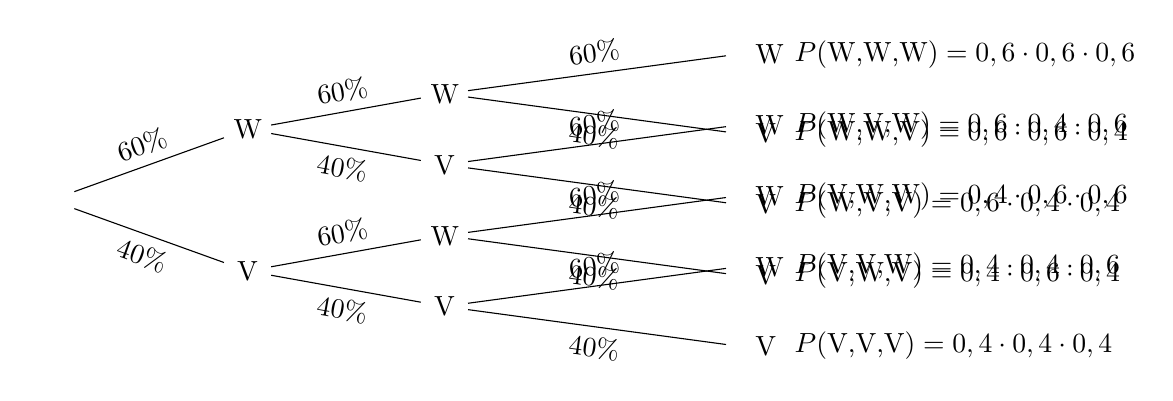
\begin{tikzpicture}[grow=right, sloped]
\node[bag] {}
    child {
        node[bag] {V}        
           child {
                node[bag] {V}
                child {
                    node[end, label=right: {V}] {}
                    node[xshift=0.5cm,yshift=-0cm, label=right: {$P($V,V,V$)=0,4\cdot 0,4 \cdot 0,4$}] {}
                    edge from parent
                    node[below=0cm] {\hspace{0.0cm}40\%}
                }
                child {
                    node[end, label=right: {W}] {}
                    node[xshift=0.5cm,yshift=-0cm, label=right: {$P($V,V,W$)=0,4\cdot 0,4\cdot0,6$}] {}
                    edge from parent
                    node[above=0cm] {\hspace{0.0cm}60\%}
                }
                edge from parent
                node[below=0cm] {\hspace{0.0cm}40\%} 
           }
           child {
                node[bag] {W}
                child {
                    node[end, label=right: {V}] {}
                    node[xshift=0.5cm,yshift=-0cm, label=right: {$P($V,W,V$)=0,4\cdot 0,6\cdot0,4$}] {}
                    edge from parent
                    node[below=0cm] {\hspace{0.0cm}40\%}
                }    
                child {
                    node[end, label=right: {W}] {}
                    node[xshift=0.5cm,yshift=-0cm, label=right: {$P($V,W,W$)=0,4\cdot0,6\cdot 0,6$}] {}
                    edge from parent
                    node[above=0cm] {\hspace{0.0cm}60\%}
                }
                edge from parent
                node[above=0cm] {\hspace{0.0cm}60\%} 
            }
        edge from parent
        node[below=0cm] {\hspace{0.0cm}40\%} 
    }
    child {
        node[bag] {W}        
           child {
                node[bag] {V}
                child {
                    node[end, label=right: {V}] {}
                    node[xshift=0.5cm,yshift=-0cm, label=right: {$P($W,V,V$)=0,6\cdot0,4\cdot0,4$}] {}
                    edge from parent
                    node[below=0cm] {\hspace{0.0cm}40\%}
                }
                child {
                    node[end, label=right: {W}] {}
                    node[xshift=0.5cm,yshift=-0cm, label=right: {$P($W,V,W$)=0,6\cdot0,4\cdot0,6$}] {}
                    edge from parent
                    node[above=0cm] {\hspace{0.0cm}60\%}
                }
                edge from parent
                node[below=0cm] {\hspace{0.0cm}40\%} 
           }
           child {
                node[bag] {W}
                child {
                    node[end, label=right: {V}] {}
                    node[xshift=0.5cm,yshift=-0cm, label=right: {$P($W,W,V$)=0,6\cdot0,6\cdot0,4$}] {}
                    edge from parent
                    node[below=0cm] {\hspace{0.0cm}40\%}
                }    
                child {
                    node[end, label=right: {W}] {}
                    node[xshift=0.5cm,yshift=-0cm, label=right: {$P($W,W,W$)=0,6\cdot0,6\cdot0,6$}] {}
                    edge from parent
                    node[above=0cm] {\hspace{0.0cm}60\%}
                }
                edge from parent
                node[above=0cm] {\hspace{0.0cm}60\%} 
            }
        edge from parent
        node[above=0cm] {\hspace{0.0cm}60\%} 
        };
\end{tikzpicture}
\caption{Kansboom volleybalmatch met 3 te spelen sets}
\label{fig:volleybal_3sets}
\end{afbeeldingenv}
%einde figuur

\section{Telbomen in de tweede graad}

\subsection{Een goed voorbeeld als instap}
Van de twee voorbeelden hierboven sluit het volleybalvoorbeeld het meest aan bij een realistische context. Wel zal elke volleyballer in de klas de opgave gekunsteld vinden doordat bij een volleybalmatch volgens de spelregels soms meer dan drie sets gespeeld moeten worden. We stellen de volgende aangepaste opgave voor. 
\begin{kader}{Opgave}{Aangepast}
De volleybalclub van Samir speelt dit weekend een wedstrijd tegen één andere ploeg. De ploeg die eerst 3 sets wint, wint de match. Als beide ploegen 2 sets winnen, is er een gelijkstand 2-2 en wordt er een vijfde beslissende set gespeeld. Een match kan dus bestaan uit 3, 4 of 5 sets. Afhankelijk van het spelverloop duurt de match kort of lang. Hoeveel mogelijke spelverlopen zijn er bij één wedstrijd? 
\end{kader}

Je vindt alle mogelijkheden in \autoref{fig:volleybal_max5sets} hieronder. 

%begin figuur
\begin{afbeeldingenv}
% Set the overall layout of the tree
\tikzstyle{level 1}=[level distance=0.5cm, sibling distance=5.0cm]
\tikzstyle{level 2}=[level distance=0.7cm, sibling distance=2.6cm]
\tikzstyle{level 3}=[level distance=1cm, sibling distance=1.4cm]
\tikzstyle{level 4}=[level distance=1cm, sibling distance=0.6cm]
\tikzstyle{level 5}=[level distance=1cm, sibling distance=0.4cm]

% Define styles for bags and leafs
\tikzstyle{bag} = [text width=1em, text centered]

\hspace{0.2cm}set 1 \hspace{0.0cm}set 2 \hspace{0.1cm}set 3 \hspace{0.1cm}set 4 \hspace{0.1cm}set 5 \hspace{0.3cm}spelverloop
\\
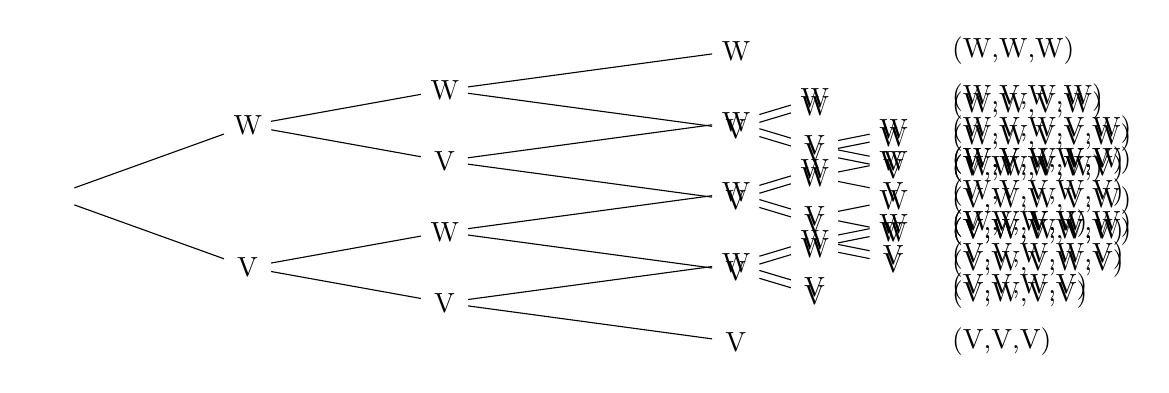
\begin{tikzpicture}[grow=right, sloped]
%wortel
\node[bag] {}
%begin level1-V
    child {
        node[bag] {V}        
%begin level2-VV
        child {
                node[bag] {V}
%begin level3-VVV
                child {
                    node[bag] {V}
                    node[xshift=2.5cm,yshift=-0cm, label=right: {(V,V,V)}] {}
                    edge from parent
                }
%end level 3-VVV
%begin level3-VVW
                child {
                    node[bag] {W}
%begin level4-VVWV
                    child {
                    node[bag] {V}
                    node[xshift=1.5cm,yshift=-0cm, label=right: {(V,V,W,V)}] {}
                    edge from parent
                    }
%end level4-VVWV
%begin level4-VVWW
                    child {
                    node[bag] {W}
%begin level5-VVWWV
                         child {
                         node[bag] {V}
                         node[xshift=0.5cm,yshift=-0cm, label=right: {(V,V,W,W,V)}] {}
                         edge from parent
                         }
%end level5-VVWWV
%begin level5-VVWWW
                         child {
                         node[bag] {W}
                         node[xshift=0.5cm,yshift=-0cm, label=right: {(V,V,W,W,W)}] {}
                         edge from parent
                         }
%end level5-VVWWW
                    edge from parent
                    }
%end level4-VVWW                    
                    edge from parent
                }
%end level3-VVW
                edge from parent
           }
%end level2-VV
%begin level2-VW
           child {
                node[bag] {W}
%begin level3-VWV
                child {
                    node[bag] {V}
%begin level4-VWVV
                    child {
                         node[bag] {V}
                         node[xshift=1.5cm,yshift=-0cm, label=right: {(V,W,V,V)}] {}
                         edge from parent                    
                    }
%end level4-VWVV
%begin level4-VWVW
                    child {
                         node[bag] {W}
%begin level5-VWVWV
                         child {
                              node[bag] {V}
                              node[xshift=0.5cm,yshift=-0cm, label=right: {(V,W,V,W,V)}] {}
                              edge from parent
                         }
%end level5-VWVWV
%begin level5-VWVWW
                         child {
                              node[bag] {W}
                              node[xshift=0.5cm,yshift=-0cm, label=right: {(V,W,V,W,W)}] {}
                              edge from parent
                         }
%end level5-VWVWW
                         edge from parent
                    }
%end level4-VWVW
                    edge from parent
                }    
%end level3-VWV
%begin level3-VWW
                child {
                    node[bag] {W}
%begin level4-VWWV
                    child {
                         node[bag] {V}
%begin level5-VWWVV
                         child {
                              node[bag] {V}
                              node[xshift=0.5cm,yshift=-0cm, label=right: {(V,W,W,V,V)}] {}
                              edge from parent
                         }
%end level5-VWWVV
%begin level5-VWWVW
                         child {
                              node[bag] {W}
                              node[xshift=0.5cm,yshift=-0cm, label=right: {(V,W,W,V,W)}] {}
                              edge from parent
                         }
%end level5-VWWVW
                         edge from parent
                    } 
%end level4-VWWV  
%begin level4-VWWW
                    child {
                         node[bag] {W}
                         node[xshift=1.5cm,yshift=-0cm, label=right: {(V,W,W,W)}] {}
                         edge from parent
                    }
%end level4-VWWW                    
                    edge from parent
                }
%end level3-VWW
                edge from parent
            }
%end level2-vW
        edge from parent
    }
%end level1-V
%begin level1-W
    child {
        node[bag] {W}        
%begin level2-WV
           child {
                node[bag] {V}
%begin level3-WVV
                child {
                    node[bag] {V}
%begin level4-WVVV
                    child {
                         node[bag] {V}
                         node[xshift=1.5cm,yshift=-0cm, label=right: {(W,V,V,V)}] {}
                         edge from parent
                    }
%end level4-WVVV
%begin level4-WVVW
                    child {
                         node[bag] {W}
%begin level5-WVVWV
                         child {
                              node[bag] {V}
                              node[xshift=0.5cm,yshift=-0cm, label=right: {(W,V,V,W,V)}] {}
                              edge from parent
                         }
%end level5-WVVWV                         
%begin level5-WVVWW
                         child {
                              node[bag] {W}
                              node[xshift=0.5cm,yshift=-0cm, label=right: {(W,V,V,W,W)}] {}
                              edge from parent
                         }
%end level5-WVVWW                         
                         edge from parent
                    }
%end level4-WVVW                    
                    edge from parent
                }
%end level3-WVV
%begin level3-WVW
                child {
                    node[bag] {W}
%begin level4-WVWV
                    child{
                         node[bag] {V}
%begin level5-WVWVV
                         child{
                              node[bag] {V}
                              node[xshift=0.5cm,yshift=-0cm, label=right: {(W,V,W,V,V)}] {}
                              edge from parent
                         } 
%end level5-WVWVV
%begin level5-WVWVW
                         child{
                              node[bag] {W}
                              node[xshift=0.5cm,yshift=-0cm, label=right: {(W,V,W,V,W)}] {}
                              edge from parent
                         } 
%end level5-WVWVW
                         edge from parent
                    }
%end level4-WVWV
%begin level4-WVWW
                    child {
                         node[bag] {W}
                         node[xshift=1.5cm,yshift=-0cm, label=right: {(W,V,W,W)}] {}
                         edge from parent
                    }
%end level4-WVWW
                    edge from parent
                }
%end level3-WVW
                edge from parent
           }
%end level2-WV
%begin level2-WW
           child {
                node[bag] {W}
%begin level3-WWV
                child {
                    node[bag] {V}
%begin level4-WWVV                    
                    child {
                         node[bag] {V}
%begin level5-WWVVV
                         child {
                              node[bag] {V}
                              node[xshift=0.5cm,yshift=-0cm, label=right: {(W,W,V,V,V)}] {}
                              edge from parent
                         }
%end level5-WWVVV
%begin level5-WWVVW
                         child {
                              node[bag] {W}
                              node[xshift=0.5cm,yshift=-0cm, label=right: {(W,W,V,V,W)}] {}
                              edge from parent
                         }
%end level5-WWVVV
                         edge from parent
                    }
%end level4-WWVV
%begin level4-WWVW
                    child {
                         node[bag] {W}
                         node[xshift=1.5cm,yshift=-0cm, label=right: {(W,W,V,W)}] {}
                         edge from parent
                    }
%end level4-WWVW
                    edge from parent
                }    
%end level3-WWV
%begin level3-WWW
                child {
                    node[bag] {W}
                    node[xshift=2.5cm,yshift=-0cm, label=right: {(W,W,W)}] {}
                    edge from parent
                }
%end level3-WWW
                edge from parent
            }
%end level2-WW        
        edge from parent
        };
%end level1-W
%end wortel
\end{tikzpicture}
\caption{Telboom volleybalmatch met 3 te winnen sets}
\label{fig:volleybal_max5sets}
\end{afbeeldingenv}
%einde figuur

Wil je aansluiten bij de leefwereld van je leerlingen dan kun je je inspiratie ook halen uit andere sporten. Bijvoorbeeld: als op 12/10/2024 de voetbaluitslag in reeks ‘Eerste Provinciale Vrouwen – Antwerpen’ voor Zammel-Wuustwezel  1-2 is, kun je ook hier naar het spelverloop vragen, al levert natuurlijk enkel de einduitslag de punten op. Met het spelverloop bedoelen we dan welke ploeg de eerste, tweede of derde goal scoort.

%begin figuur
\begin{afbeeldingenv}
% Set the overall layout of the tree
\tikzstyle{level 1}=[level distance=1.2cm, sibling distance=0.75cm]
\tikzstyle{level 2}=[level distance=1.2cm, sibling distance=0.5cm]
\tikzstyle{level 3}=[level distance=1.2cm, sibling distance=0.5cm]

% Define styles for bags and leafs
\tikzstyle{bag} = [text width=1em, text centered]

\hspace{1.1cm}goal 1 \hspace{0.1cm}goal 2 \hspace{0.1cm}goal 3  \hspace{0.2cm}spelverloop
\\
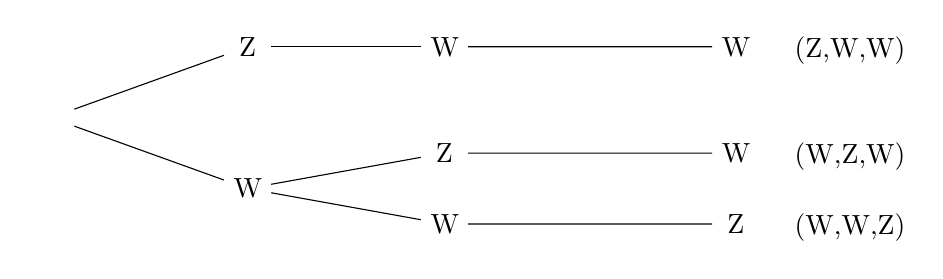
\begin{tikzpicture}[grow=right, sloped]
%wortel
\node[bag] {}
%begin level1-W
    child {
        node[bag] {W}        
%begin level2-WW
        child {
                node[bag] {W}
%begin level3-WWZ
                child {
                    node[bag] {Z}
                    node[xshift=0.5cm,yshift=-0.05cm, label=right: {(W,W,Z)}] {}
                    edge from parent
                }
%end level 3-WWZ
                edge from parent
           }
%end level2-WW
%begin level2-WZ
           child {
                node[bag] {Z}
%begin level3-WZW
                child {
                    node[bag] {W}
                    node[xshift=0.5cm,yshift=-0.05cm, label=right: {(W,Z,W)}] {}
                    edge from parent
                }    
%end level3-WZW
                edge from parent
            }
%end level2-WZ
        edge from parent
    }
%end level1-W
%begin level1-Z
    child {
        node[bag] {Z}        
%begin level2-ZW
           child {
                node[bag] {W}
%begin level3-ZWW
                child {
                    node[bag] {W}
                    node[xshift=0.5cm,yshift=-0.05cm, label=right: {(Z,W,W)}] {}
                    edge from parent
                }
%end level3-ZWW
                edge from parent
           }
%end level2-ZW
        edge from parent
        };
%end level1-Z
%end wortel
\end{tikzpicture}
\caption{Voetbalmatch met uitslag 1-2 voor Wuustwezel}
\label{fig:voetbal}
\end{afbeeldingenv}
%einde figuur

Het interessante aan beide voorbeelden is dat de telbomen niet ‘regelmatig’ zijn. Bij de volleybalmatch is de ‘afstand’ tussen een blad van de boom en de wortel niet altijd dezelfde. Zo hangt het blad met spelverloop (W,W,W) aan een opeenvolging van drie takken en het blad met spelverloop (V,W,V,W,V) aan een opeenvolging van vijf takken, zoals je in \autoref{fig:volleybal_max5sets} kunt zien. Bij de voetbalwedstrijd zijn er niet in elke knoop evenveel vertakkingen. Er zijn 3 generaties knopen. In de wortel zijn er twee vertakkingen: naar Z(ammel) en W(uustwezel). De eerste generatie krijgt de naam ‘goal 1’ en vanuit de knoop Zammel vertrekt slechts 1 tak (naar Wuustwezel), maar vanuit de knoop Wuustwezel vertrekken twee takken. De bladeren geven drietallen. Zo betekent (Z,W,W) dat Zammel de eerste goal scoorde en Wuustwezel de tweede en derde. 

Deze ‘onregelmatigheid’ maakt dat de beide voorbeelden betere instapvoorbeelden zijn dan het volgende probleem uit Pienter (Descheermaeker et al. 2022). 
\afbeelding{img/2A2menu.jpg}{Driegangenmenu}{menu}
We maken een telboom die alle mogelijkheden weergeeft.

Tussen de wortel en elk van de bladeren zit telkens een opeenvolging van drie takken, maar het aantal vertakkingen verschilt: uit de wortel vertrekken drie takken naar de eerste generatie knopen die de drie voorgerechten voorstellen, uit deze knopen vertrekken telkens vier takken naar de tweede generatie knopen die de hoofdgerechten voorstellen, en uit deze laatste knopen vertrekken telkens twee takken want er is keuze uit twee nagerechten. Het totaal aantal mogelijkheden voor het menu is dan $3\cdot4\cdot2=24$ .

%begin figuur
\begin{afbeeldingenv}
% Set the overall layout of the tree
\tikzstyle{level 1}=[level distance=1.5cm, sibling distance=3.2cm]
\tikzstyle{level 2}=[level distance=1.5cm, sibling distance=0.8cm]
\tikzstyle{level 3}=[level distance=1.5cm, sibling distance=0.4cm]

% Define styles for bags and leafs
\tikzstyle{bag} = [text width=1em, text centered]

\hspace{1.3cm}voor \hspace{0.6cm}hoofd \hspace{0.6cm}na  \hspace{0.2cm}menu
\\
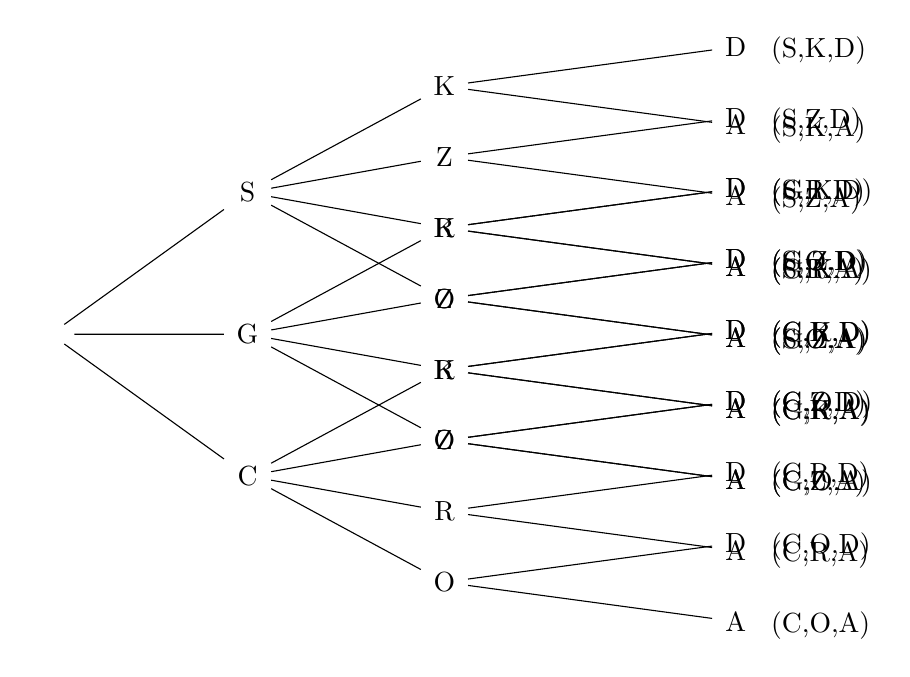
\begin{tikzpicture}[grow=right, sloped]
%wortel
\node[bag] {}
%begin level1-C
    child {
        node[bag] {C}        
%begin level2-CO
        child {
                node[bag] {O}
%begin level3-COA
                child {
                    node[bag] {A}
                    node[xshift=0.2cm,yshift=-0.05cm, label=right: {(C,O,A)}] {}
                    edge from parent
                }
%end level 3-COA
%begin level3-COD
                child {
                    node[bag] {D}
                    node[xshift=0.2cm,yshift=-0.05cm, label=right: {(C,O,D)}] {}
                    edge from parent
                }
%end level 3-COD
                edge from parent
           }
%end level2-CO
%begin level2-CR
        child {
                node[bag] {R}
%begin level3-CRA
                child {
                    node[bag] {A}
                    node[xshift=0.2cm,yshift=-0.05cm, label=right: {(C,R,A)}] {}
                    edge from parent
                }
%end level 3-CRA
%begin level3-CRD
                child {
                    node[bag] {D}
                    node[xshift=0.2cm,yshift=-0.05cm, label=right: {(C,R,D)}] {}
                    edge from parent
                }
%end level 3-CRD
                edge from parent
           }
%end level2-CR
%begin level2-CZ
        child {
                node[bag] {Z}
%begin level3-CZA
                child {
                    node[bag] {A}
                    node[xshift=0.2cm,yshift=-0.05cm, label=right: {(C,Z,A)}] {}
                    edge from parent
                }
%end level 3-CZA
%begin level3-CZD
                child {
                    node[bag] {D}
                    node[xshift=0.2cm,yshift=-0.05cm, label=right: {(C,Z,D)}] {}
                    edge from parent
                }
%end level 3-CZD
                edge from parent
           }
%end level2-CZ
%begin level2-CK
        child {
                node[bag] {K}
%begin level3-CKA
                child {
                    node[bag] {A}
                    node[xshift=0.2cm,yshift=-0.05cm, label=right: {(C,K,A)}] {}
                    edge from parent
                }
%end level 3-CKA
%begin level3-CKD
                child {
                    node[bag] {D}
                    node[xshift=0.2cm,yshift=-0.05cm, label=right: {(C,K,D)}] {}
                    edge from parent
                }
%end level 3-CKD
                edge from parent
           }
%end level2-CK
        edge from parent
    }
%end level1-C
%begin level1-G
    child {
        node[bag] {G}        
%begin level2-GO
        child {
                node[bag] {O}
%begin level3-GOA
                child {
                    node[bag] {A}
                    node[xshift=0.2cm,yshift=-0.05cm, label=right: {(G,O,A)}] {}
                    edge from parent
                }
%end level 3-GOA
%begin level3-GOD
                child {
                    node[bag] {D}
                    node[xshift=0.2cm,yshift=-0.05cm, label=right: {(G,O,D)}] {}
                    edge from parent
                }
%end level 3-GOD
                edge from parent
           }
%end level2-GO
%begin level2-GR
        child {
                node[bag] {R}
%begin level3-GRA
                child {
                    node[bag] {A}
                    node[xshift=0.2cm,yshift=-0.05cm, label=right: {(G,R,A)}] {}
                    edge from parent
                }
%end level 3-GRA
%begin level3-GRD
                child {
                    node[bag] {D}
                    node[xshift=0.2cm,yshift=-0.05cm, label=right: {(G,R,D)}] {}
                    edge from parent
                }
%end level 3-GRD
                edge from parent
           }
%end level2-GR
%begin level2-GZ
        child {
                node[bag] {Z}
%begin level3-GZA
                child {
                    node[bag] {A}
                    node[xshift=0.2cm,yshift=-0.05cm, label=right: {(G,Z,A)}] {}
                    edge from parent
                }
%end level 3-GZA
%begin level3-GZD
                child {
                    node[bag] {D}
                    node[xshift=0.2cm,yshift=-0.05cm, label=right: {(G,Z,D)}] {}
                    edge from parent
                }
%end level 3-GZD
                edge from parent
           }
%end level2-GZ
%begin level2-GK
        child {
                node[bag] {K}
%begin level3-GKA
                child {
                    node[bag] {A}
                    node[xshift=0.2cm,yshift=-0.05cm, label=right: {(G,K,A)}] {}
                    edge from parent
                }
%end level 3-GKA
%begin level3-GKD
                child {
                    node[bag] {D}
                    node[xshift=0.2cm,yshift=-0.05cm, label=right: {(G,K,D)}] {}
                    edge from parent
                }
%end level 3-GKD
                edge from parent
           }
%end level2-GK
        edge from parent
    }
%end level1-G
%begin level1-S
    child {
        node[bag] {S}        
%begin level2-SO
        child {
                node[bag] {O}
%begin level3-SOA
                child {
                    node[bag] {A}
                    node[xshift=0.2cm,yshift=-0.05cm, label=right: {(S,O,A)}] {}
                    edge from parent
                }
%end level 3-SOA
%begin level3-SOD
                child {
                    node[bag] {D}
                    node[xshift=0.2cm,yshift=-0.05cm, label=right: {(S,O,D)}] {}
                    edge from parent
                }
%end level 3-SOD
                edge from parent
           }
%end level2-SO
%begin level2-SR
        child {
                node[bag] {R}
%begin level3-SRA
                child {
                    node[bag] {A}
                    node[xshift=0.2cm,yshift=-0.05cm, label=right: {(S,R,A)}] {}
                    edge from parent
                }
%end level 3-SRA
%begin level3-SRD
                child {
                    node[bag] {D}
                    node[xshift=0.2cm,yshift=-0.05cm, label=right: {(S,R,D)}] {}
                    edge from parent
                }
%end level 3-SRD
                edge from parent
           }
%end level2-SR
%begin level2-SZ
        child {
                node[bag] {Z}
%begin level3-SZA
                child {
                    node[bag] {A}
                    node[xshift=0.2cm,yshift=-0.05cm, label=right: {(S,Z,A)}] {}
                    edge from parent
                }
%end level 3-SZA
%begin level3-SZD
                child {
                    node[bag] {D}
                    node[xshift=0.2cm,yshift=-0.05cm, label=right: {(S,Z,D)}] {}
                    edge from parent
                }
%end level 3-SZD
                edge from parent
           }
%end level2-SZ
%begin level2-SK
        child {
                node[bag] {K}
%begin level3-SKA
                child {
                    node[bag] {A}
                    node[xshift=0.2cm,yshift=-0.05cm, label=right: {(S,K,A)}] {}
                    edge from parent
                }
%end level 3-SKA
%begin level3-SKD
                child {
                    node[bag] {D}
                    node[xshift=0.2cm,yshift=-0.05cm, label=right: {(S,K,D)}] {}
                    edge from parent
                }
%end level 3-SKD
                edge from parent
           }
%end level2-SK
        edge from parent
    };
%end level1-S
%end wortel
\end{tikzpicture}
\caption{Driegangenmenu}
\label{fig:menu}
\end{afbeeldingenv}
%einde figuur



Dit gekende ‘menuprobleem’ is een zeer toegankelijk voorbeeld en dat is wellicht de reden dat we het in bijna alle handboeken die we raadpleegden tegenkomen. Het leidt tot een regelmatige telboom. Dit kan bij leerlingen de misconceptie doen ontstaan dat er per generatie uit elke knoop telkens evenveel takken moeten vertrekken. Het vormt echter alvast een beter voorbeeld dan een probleem dat tot een telboom leidt waarbij uit elke knoop, ongeacht de generatie, exact evenveel takken vertrekken. Een ander aandachtspunt om al dan niet voor dit voorbeeld te kiezen is de grootte van de telboom in relatie tot de moeilijkheidsgraad van het probleem. Omwille van het relatief eenvoudige probleem loop je het risico snelle leerlingen kwijt te raken omdat ze het nut niet inzien tot het tekenen van zo’n grote telboom. Het voorbeeld is voor hen te eenvoudig. Zij zien onmiddellijk in dat het totaal aantal mogelijkheden 24 zal zijn. 

\subsection{Telbomen leren opstellen}

We nemen het voorbeeld over de volleybalmatch waarbij de ploegen juist drie sets spelen. Bij de telboom in \autoref{volley} hoort de volgende opgave.

\end{multicols}
 

\afbeelding{img/2B1Volleyopgave.jpg}{Opgave volleybalclub Samir}{volleyopgave}

\begin{multicols}{2} %
Door in a) de voorstelling te bepalen en in b) het schema voor te structuren zoals in \autoref{volley}, ontneem je de leerlingen de kans om zelf een schema te maken en hun eigen ideeën te ontwikkelen. Het belangrijke denkwerk is voor de leerlingen gedaan en zij moeten enkel invullen. 

Het is interessanter om leerlingen bij deze opgave eerst zelf te laten proberen zonder dat je dit van bij aanvang stuurt. Op die manier zorg je voor een beter begrip van het probleem en leer je hoe leerlingen aan een probleem beginnen. Sommigen starten misschien met een bruikbaar schema of elementen die je kunt gebruiken bij het opstellen van de telboom. 

Om telbomen te leren opstellen is het zinvol leerlingen voorbeelden van telbomen voor te schotelen en hen vragen te stellen over de betekenis van de verschillende generaties knopen en de bladeren. Bij het vlaggenprobleem kun je bijvoorbeeld vragen wat (G,Z,R) betekent of kun je vragen om de vlag te tekenen die hoort bij (Z,G,R). 

De vraag in \autoref{kamers} is een heel mooie vraag die expliciet peilt naar de betekenis van de knopen en dus zeker bij het aanbrengen van telproblemen een plaats verdient. We vonden de opgave o.a. in het handboek Delta Nova 5 (De Loddere et al. 2009). Het bepalen van de juiste generaties knopen is cruciaal bij het opstellen van een telboom. Het is net daar dat leerlingen vaak een denkfout maken. Deze vraag doet hen precies stilstaan bij de betekenis. Het is interessant om stil te staan bij de betekenis van beide schema's. Als we in het schema van de vader de bovenste opeenvolging van takken volgen, zou kamer 1 zowel wit, lichtgeel als lichtgroen geschilderd worden en kamer 2 geen kleur krijgen. Dit klopt niet. Volgen we dezelfde eerste opeenvolging van takken in het schema van de zoon dan schildert vader zowel kamer 1 als 2 wit. De zoon heeft het juiste schema gemaakt.

\end{multicols}
\afbeelding [12cm]{img/2B2Kamers.png}{Kamers schilderen}{kamers}

\begin{multicols}{2}

We stellen ook een paar wijzigingen voor bij de opgave. Zoals hierboven al aangehaald geven we er in deze loep de voorkeur aan om te spreken over een telboom en zien we de naam boomschema als een overkoepelende naam. Verder merken we dat de bladeren niet benoemd zijn. Tot slot zouden de kleuren beter wit, blauw en groen zijn omdat we dan gemakkelijker met afkortingen kunnen werken en een blad in de telboom van de zoon bijvoorbeeld kunnen benoemen met (W,G): de vader schildert kamer 1 wit en kamer 2 groen.

Ten slotte is het relevant te benadrukken dat het gebruik van telbomen een volgorde vastlegt. Soms is deze volgorde vanzelfsprekend: zo spreken we bij de voorbeelden hierboven van de eerste set, de eerste kamer, het voorgerecht… In andere gevallen zul je ‘kunstmatig’ een volgorde moeten aanbrengen, zoals in het volgende voorbeeld. Een kaartspel bestaat uit 52 kaarten, verdeeld in vier kleuren met elk dertien kaarten nl. harten, ruiten, klaveren en schoppen. De naam kleur kan verwarrend zijn omdat dit niet om de fysieke kleuren rood en zwart gaat. Het is echter de gebruikelijke benaming voor de vier soorten kaarten in een kaartspel. We nemen uit het kaartspel enkel de harten en schoppen kaarten en vormen zo een set van 26 kaarten. We trekken uit dit kaartspel twee kaarten en letten enkel op de kleur van de twee getrokken kaarten. We willen het aantal mogelijkheden tellen om dit te doen. Om dit in een telboom te kunnen voorstellen, brengen we een volgorde aan: we trekken een eerste kaart en vervolgens een tweede kaart (zonder de eerste kaart terug te leggen). Je vindt de telboom in de onderstaande figuur.

%begin figuur
\begin{afbeeldingenv}
% Set the overall layout of the tree
\tikzstyle{level 1}=[level distance=2cm, sibling distance=1.6cm]
\tikzstyle{level 2}=[level distance=1.5cm, sibling distance=0.8cm]

% Define styles for bags and leafs
\tikzstyle{bag} = [text width=1em, text centered]
\small
\hspace{2.4cm}kaart 1 \hspace{0.3cm}kaart 2 \hspace{0.1cm}getrokken
\\
\hspace{4.6cm}kaarten
\\
\normalsize
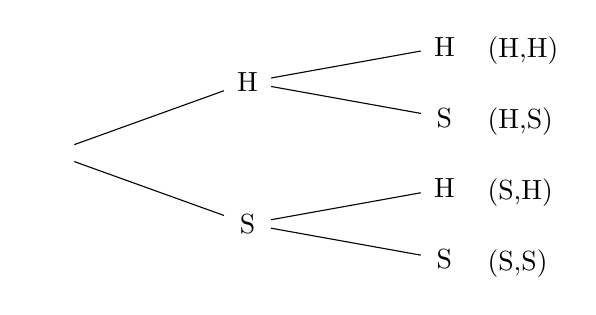
\begin{tikzpicture}[grow=right, sloped]
%wortel
\node[bag] {}
%begin level1-S
    child {
        node[bag] {S}        
%begin level2-SS
        child {
                node[bag] {S}
                node[xshift=0.3cm,yshift=-0.05cm, label=right: {(S,S)}] {}
                edge from parent
                }
%end level2-SS
%begin level2-SH
        child {
                node[bag] {H}
                node[xshift=0.3cm,yshift=-0.05cm, label=right: {(S,H)}] {}
                edge from parent
        }        
%end level2-SH
        edge from parent
    }
%end level1-S
%begin level1-H
    child {
        node[bag] {H}        
%begin level2-HS
        child {
                node[bag] {S}
                node[xshift=0.3cm,yshift=-0.05cm, label=right: {(H,S)}] {}
                edge from parent
           }
%end level2-HS
%begin level2-HH
        child {
                node[bag] {H}
                node[xshift=0.3cm,yshift=-0.05cm, label=right: {(H,H)}] {}
                edge from parent
           }
%end level2-HH
        edge from parent
    };
%end level1-H
%end wortel
\end{tikzpicture}
\caption{Telboom: 2 kaarten uit onvolledig kaartspel}
\label{fig:kaarten_versie01}
\end{afbeeldingenv}
%einde figuur

We lossen de volgende vragen op met deze telboom. 
\begin{vraagenantwoord} 
\vraag{Hoeveel mogelijke combinaties van 2 kleuren kun je trekken als het wél uitmaakt welke kaart je als eerste of tweede trekt?} 
\antwoord{In deze situatie stellen we de mogelijkheden voor met koppels omdat de volgorde belangrijk is. Het antwoord is $4$ nl.$ (H,H),(H,S),(S,H),(S,S)$.} 
\vraag{Hoeveel mogelijke combinaties van 2 verschillende kleuren kun je trekken als het niet uitmaakt welke kaart je als eerste of tweede trekt?}
\antwoord{In deze situatie is de volgorde niet belangrijk en tellen de twee uitkomsten (H,S),(S,H) voor $1$ omdat ze allebei de situatie $1$ Harten en $1$ Schoppen voorstellen. De twee bladeren (H,S),(S,H) mogen we dus niet allebei tellen. Als we symbolisch willen voorstellen dat de volgorde niet uitmaakt, kunnen we notatie met een verzameling gebruiken \{H,S\}. Er is hier dus maar 1 mogelijkheid.}
\end{vraagenantwoord}

\subsection{Vereenvoudigde telbomen}
Bij een te groot aantal vertakkingen bij de generaties knopen vraagt het te veel werk om de telboom te tekenen en wordt hij onoverzichtelijk. Bovendien zijn sommige telproblemen zo eenvoudig dat zeker sterke leerlingen het nut om de telboom te tekenen dan al snel niet meer inzien. Het blijft echter zinvol om de telboom op te starten om zo zicht te krijgen op het probleem. Eens het probleem duidelijk is, kun je overstappen op een ‘vereenvoudigde telboom’, een term die geïnspireerd is op de handboekenreeks Delta, waar over een ‘vereenvoudigd boomdiagram’ gesproken wordt. Hierbij bundelt men sommige takken en noteert men het aantal takken bij elke tak.

We hernemen het voorbeeld van het kaartspel met enkel de kleuren harten en schoppen en verfijnen het. Elke kleur bestaat uit 13 kaarten: aas, 2, …, 10, boer, dame en heer. Uit het kaartspel nemen we 4 harten en 2 schoppen. Bijvoorbeeld: harten 2 (H2), harten 5 (H5), harten 8 (H8), harten dame (HD), schoppenaas (SA) en schoppenboer (SB). We trekken uit dit stapeltje van zes kaarten twee kaarten achter elkaar zonder ze terug te leggen. We willen weer het aantal mogelijkheden tellen om dit te doen. 

In \autoref{fig:kaarten_versie02} tekenen we de niet-vereenvoudigde telboom. In \autoref{fig:kaarten_versie03} staat de vereenvoudigde, waarbij telkens het aantal kaarten van een kleur bij de tak staat. Meer bepaald staat in de vereenvoudigde telboom dus een 4 boven de tak van de wortel naar de uitkomst ‘H’arten bij de eerste trekking. Dit betekent dat de 4 rode takken voor kaart 1 uit \autoref{fig:kaarten_versie02} samengenomen zijn tot 1 rode tak in \autoref{fig:kaarten_versie03}. Bij de tak die van hieruit naar de uitkomst S bij de tweede trekking gaat, staat een 2, wat betekent dat elk van die oorspronkelijke 4 rode takken in zijn eindknoop vertakt in 2 zwarte takken naar een schoppen. Vanuit de wortel naar het blad (H,S) zijn er dus $4\cdot2=8$ opeenvolgingen van takken. Bijgevolg noteren we bij dit blad dat er 8 mogelijkheden zijn om eerst een harten en dan een schoppen te trekken.



%begin figuur 1
\begin{afbeeldingenv}
% Set the overall layout of the tree
\tikzstyle{level 1}=[level distance=1.7cm, sibling distance=2.0cm]
\tikzstyle{level 2}=[level distance=2cm, sibling distance=0.4cm]

% Define styles for bags and leafs
\tikzstyle{bag} = [text width=2em, text centered]


\small
\hspace{1.4cm}kaart 1 \hspace{0.9cm}kaart 2 \hspace{0.2cm}getrokken
\\
\hspace{4.6cm}kaarten
\\
\normalsize
%\hspace{1.4cm}kaart 1 \hspace{2cm}kaart 2 \hspace{0.1cm}getrokken kaarten
%\\
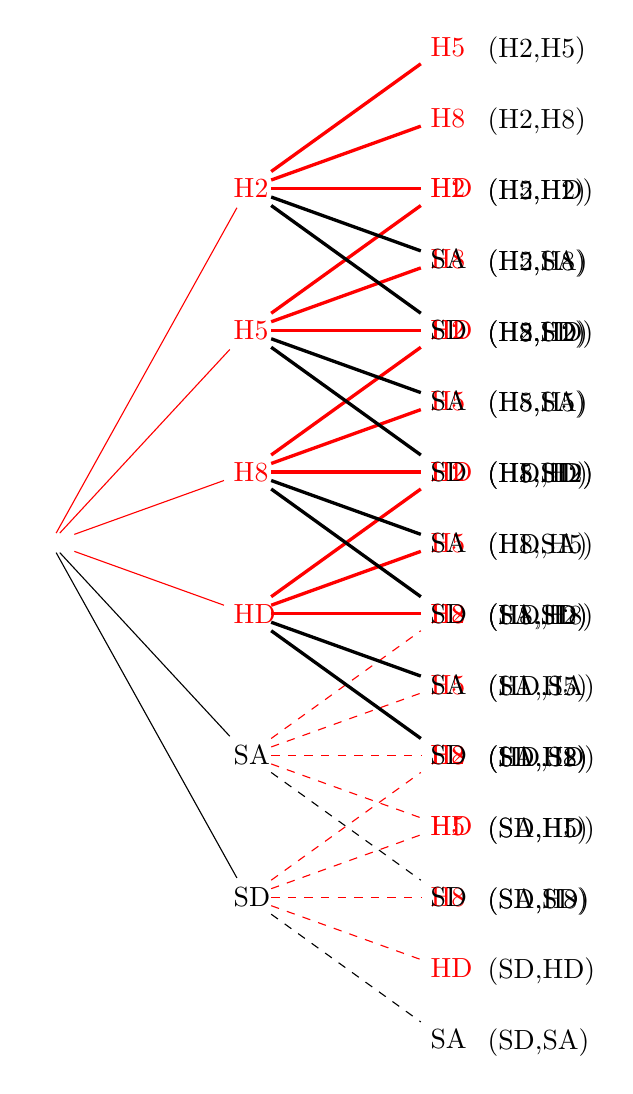
\begin{tikzpicture}[grow=right, sloped]
%wortel
\node[bag] {}
%begin level1-SD
    child {
        node[bag] {SD}        
%begin level2-SD-SA
        child {
                node[bag] {SA}
                node[xshift=0.3cm,yshift=-0.05cm, label=right: {(SD,SA)}] {}
                edge from parent[dashed]
        }
%end level2-SD-SA
%begin level2-SD-HD
        child {
                node[bag,red] {HD}
                node[xshift=0.3cm,yshift=-0.05cm, label=right: {(SD,HD)}] {}
                edge from parent[red,dashed]
           }
%end level2-SD-H8
%begin level2-SD-H8
        child {
                node[bag,red] {H8}
                node[xshift=0.3cm,yshift=-0.05cm, label=right: {(SD,H8)}] {}
                edge from parent[red,dashed]
           }
%end level2-SD-H8
%begin level2-SD-H5
        child {
                node[bag,red] {H5}
                node[xshift=0.3cm,yshift=-0.05cm, label=right: {(SD,H5)}] {}
                edge from parent[red,dashed]
           }
%end level2-SD-H5
%begin level2-SD-H2
        child {
                node[bag, red] {H2}
                node[xshift=0.3cm,yshift=-0.05cm, label=right: {(SD,H2)}] {}
                edge from parent[red,dashed]
           }
%end level2-SD-H2
        edge from parent
    }
%end level1-SD
%begin level1-SA
    child {
        node[bag] {SA}        
%begin level2-SA-SD
        child {
                node[bag] {SD}
                node[xshift=0.3cm,yshift=-0.05cm, label=right: {(SA,SD)}] {}
                edge from parent[dashed]
           }
%end level2-SA-SD
%begin level2-SA-HD
        child {
                node[bag,red] {HD}
                node[xshift=0.3cm,yshift=-0.05cm, label=right: {(SA,HD)}] {}
                edge from parent[red,dashed]
           }
%end level2-SA-HD
%begin level2-SA-H8
        child {
                node[bag,red] {H8}
                node[xshift=0.3cm,yshift=-0.05cm, label=right: {(SA,H8)}] {}
                edge from parent[red,dashed]
           }
%end level2-SA-H8
%begin level2-SA-H5
        child {
                node[bag,red] {H5}
                node[xshift=0.3cm,yshift=-0.05cm, label=right: {(SA,H5)}] {}
                edge from parent[red,dashed]
           }
%end level2-SA-H5
%begin level2-SA-H2
        child {
                node[bag, red] {H2}
                node[xshift=0.3cm,yshift=-0.05cm, label=right: {(SA,H2)}] {}
                edge from parent[red,dashed]
           }
%end level2-SA-H2
        edge from parent
    }
%end level1-SA
%begin level1-HD
    child {
        node[bag,red] {HD}        
%begin level2-HD-SD
        child {
                node[bag] {SD}
                node[xshift=0.3cm,yshift=-0.05cm, label=right: {(HD,SD)}] {}
                edge from parent[black, very thick]
           }
%end level2-HD-SD
%begin level2-HD-SA
        child {
                node[bag] {SA}
                node[xshift=0.3cm,yshift=-0.05cm, label=right: {(HD,SA)}] {}
                edge from parent[black, very thick]
           }
%end level2-HD-SA
%begin level2-HD-H8
        child {
                node[bag,red] {H8}
                node[xshift=0.3cm,yshift=-0.05cm, label=right: {(HD,H8)}] {}
                edge from parent[red, very thick]
           }
%end level2-HD-H8
%begin level2-HD-H5
        child {
                node[bag,red] {H5}
                node[xshift=0.3cm,yshift=-0.05cm, label=right: {(HD,H5)}] {}
                edge from parent[red, very thick]
           }
%end level2-HD-H5
%begin level2-HD-H2
        child {
                node[bag, red] {H2}
                node[xshift=0.3cm,yshift=-0.05cm, label=right: {(HD,H2)}] {}
                edge from parent[red, very thick]
           }
%end level2-HD-H2
        edge from parent[red]
    }
%end level1-HD
%begin level1-H8
    child {
        node[bag,red] {H8}        
%begin level2-H8-SD
        child {
                node[bag] {SD}
                node[xshift=0.3cm,yshift=-0.05cm, label=right: {(H8,SD)}] {}
                edge from parent[black, very thick]
           }
%end level2-H8-SD
%begin level2-H8-SA
        child {
                node[bag] {SA}
                node[xshift=0.3cm,yshift=-0.05cm, label=right: {(H8,SA)}] {}
                edge from parent[black, very thick]
           }
%end level2-H8-SA
%begin level2-H8-HD
        child {
                node[bag,red] {HD}
                node[xshift=0.3cm,yshift=-0.05cm, label=right: {(H8,HD)}] {}
                edge from parent[red, very thick]
           }
%end level2-H8-HD
%begin level2-H8-H5
        child {
                node[bag,red] {H5}
                node[xshift=0.3cm,yshift=-0.05cm, label=right: {(H8,H5)}] {}
                edge from parent[red, very thick]
           }
%end level2-H8-H5
%begin level2-H8-H2
        child {
                node[bag,red] {H2}
                node[xshift=0.3cm,yshift=-0.05cm, label=right: {(H8,H2)}] {}
                edge from parent[red, very thick]
           }
%end level2-H8-H2
        edge from parent[red]
    }
%end level1-H8
%begin level1-H5
    child {
        node[bag,red] {H5}        
%begin level2-H5-SD
        child {
                node[bag] {SD}
                node[xshift=0.3cm,yshift=-0.05cm, label=right: {(H5,SD)}] {}
                edge from parent[black, very thick]
           }
%end level2-H5-SD
%begin level2-H5-SA
        child {
                node[bag] {SA}
                node[xshift=0.3cm,yshift=-0.05cm, label=right: {(H5,SA)}] {}
                edge from parent[black, very thick]
           }
%end level2-H5-SA
%begin level2-H5-HD
        child {
                node[bag,red] {HD}
                node[xshift=0.3cm,yshift=-0.05cm, label=right: {(H5,HD)}] {}
                edge from parent[red, very thick]
           }
%end level2-H5-HD
%begin level2-H5-H8
        child {
                node[bag,red] {H8}
                node[xshift=0.3cm,yshift=-0.05cm, label=right: {(H5,H8)}] {}
                edge from parent[red, very thick]
           }
%end level2-H5-H8
%begin level2-H5-H2
        child {
                node[bag,red] {H2}
                node[xshift=0.3cm,yshift=-0.05cm, label=right: {(H5,H2)}] {}
                edge from parent[red, very thick]
           }
%end level2-H5-H2
        edge from parent[red]
    }
%end level1-H5
%begin level1-H2
    child {
        node[bag,red] {H2}        
%begin level2-H2-SD
        child {
                node[bag] {SD}
                node[xshift=0.3cm,yshift=-0.05cm, label=right: {(H2,SD)}] {}
                edge from parent[black, very thick]
           }
%end level2-H2-SD
%begin level2-H2-SA
        child {
                node[bag] {SA}
                node[xshift=0.3cm,yshift=-0.05cm, label=right: {(H2,SA)}] {}
                edge from parent[black, very thick]
           }
%end level2-H2-SA
%begin level2-H2-HD
        child {
                node[bag,red] {HD}
                node[xshift=0.3cm,yshift=-0.05cm, label=right: {(H2,HD)}] {}
                edge from parent[red, very thick]
           }
%end level2-H2-HD
%begin level2-H2-H8
        child {
                node[bag,red] {H8}
                node[xshift=0.3cm,yshift=-0.05cm, label=right: {(H2,H8)}] {}
                edge from parent[red, very thick]
           }
%end level2-H2-H8
%begin level2-H2-H5
        child {
                node[bag, red] {H5}
                node[xshift=0.3cm,yshift=-0.05cm, label=right: {(H2,H5)}] {}
                edge from parent[red, very thick]
           }
%end level2-H2-H5
        edge from parent[red]
    };
%end level1-H2
%end wortel
\end{tikzpicture}
\caption{Telboom harten en schoppen}
\label{fig:kaarten_versie02}
\end{afbeeldingenv}
%einde figuur 1





%begin figuur 2
\begin{afbeeldingenv}
% Set the overall layout of the tree
\tikzstyle{level 1}=[level distance=1.5cm, sibling distance=1.6cm]
\tikzstyle{level 2}=[level distance=1.8cm, sibling distance=0.8cm]

% Define styles for bags and leafs
\tikzstyle{bag} = [text width=1em, text centered]

\hspace{1.2cm}kaart 1 \hspace{0.5cm}kaart 2 \hspace{0.0cm}getrokken kaarten
\\
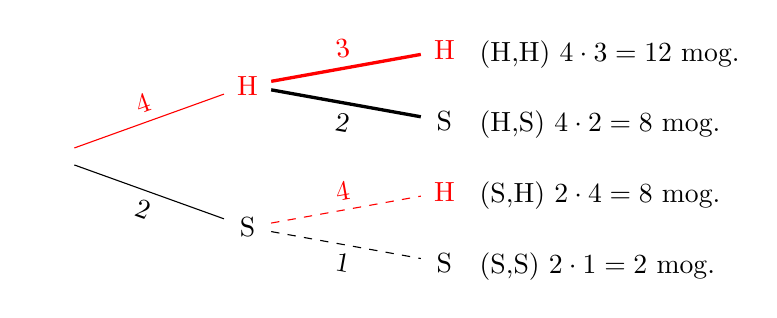
\begin{tikzpicture}[grow=right, sloped]
%wortel
\node[bag] {}
%begin level1-S
    child {
        node[bag] {S}        
%begin level2-SS
        child {
                node[bag] {S}
                node[xshift=0.2cm,yshift=-0.05cm, label=right: {(S,S) $2\cdot1=2$ mog.}] {}
                edge from parent[dashed]
                node[below=0.0cm] {1}
                }
%end level2-SS
%begin level2-SH
        child {
                node[bag,red] {H}
                node[xshift=0.2cm,yshift=-0.05cm, label=right: {(S,H) $2\cdot4=8$ mog. }] {}
                edge from parent[red,dashed]
                node[above=0.0cm,red] {4}
        }        
%end level2-SH
        edge from parent
        node[below=0.0cm] {2}
    }
%end level1-S
%begin level1-H
    child {
        node[bag,red] {H}        
%begin level2-HS
        child {
                node[bag] {S}
                node[xshift=0.2cm,yshift=-0.05cm, label=right: {(H,S) $4\cdot2=8$ mog.}] {}
                edge from parent[black,very thick]
                node[below=0.0cm] {2}
           }
%end level2-HS
%begin level2-HH
        child {
                node[bag,red] {H}
                node[xshift=0.2cm,yshift=-0.05cm, label=right: {(H,H) $4\cdot3=12$ mog.}] {}
                edge from parent[red,very thick]
                node[above=0.0cm, red] {3}
           }
%end level2-HH
        edge from parent[red]
        node[above=0.0cm] {4}
    };
%end level1-H
%end wortel
\end{tikzpicture}
\caption{Vereenvoudigde telboom harten en schoppen}
\label{fig:kaarten_versie03}
\end{afbeeldingenv}
%einde figuur 2

Het is duidelijk dat de informatie over welke kaart het precies gaat, hierbij verloren gaat. Je houdt enkel de informatie over de kleur over. De vereenvoudigde telboom maakt abstractie van de eigenschap ‘welke kaart precies’ en houdt enkel de eigenschap ‘welke kleur’ over waardoor de leerling abstracter moet kunnen denken.

Een vereenvoudigde telboom bij het driegangenmenu ziet eruit als volgt:
 
%begin figuur
\begin{afbeeldingenv}
% Set the overall layout of the tree
\tikzstyle{level 1}=[level distance=1.5cm, sibling distance=3.2cm]
\tikzstyle{level 2}=[level distance=1.5cm, sibling distance=0.8cm]
\tikzstyle{level 3}=[level distance=1.5cm, sibling distance=0.4cm]

% Define styles for bags and leafs
\tikzstyle{bag} = [text width=0.5em, text centered]

\hspace{0.5cm}voor \hspace{0.6cm}hoofd \hspace{0.8cm}na  \hspace{0.5cm}aantal menu's
\\
\begin{tikzpicture}[grow=right, sloped]
%wortel
\node[bag] {}
%begin level1-C
    child {
        node[bag] {}        
%begin level2-CO
        child {
                node[bag] {}
%begin level3-COA
                child {
                    node[bag] {}
                    node[xshift=0.0cm,yshift=-0.05cm, label=right: {$3\cdot4\cdot2=24$}] {}
                    edge from parent
                    node[above=0.0cm] {$2$}
                }
%end level 3-COA
                edge from parent
                node[above=0.0cm] {$4$}
           }
%end level2-CO
        edge from parent
        node[above=0.0cm] {$3$}
    };
%end level1-C
%end wortel
\end{tikzpicture}
\caption{Vereenvoudigde telboom Driegangenmenu}
\label{fig:menu_vereenvoudigd}
\end{afbeeldingenv}
%einde figuur
    
\subsubsection{De bladeren veranderen van betekenis}
Bij de overgang naar een vereenvoudigde telboom krijgen de bladeren een bijkomende betekenis. Bij de niet-vereenvoudigde boom geeft elk blad een mogelijke trekking, bijvoorbeeld (H2,SA). De vereenvoudigde boom geeft nog altijd weer welke mogelijkheden er zijn, bijvoorbeeld (H,S) zonder de specifieke kaarten te vermelden, maar geeft nu ook het aantal mogelijkheden weer om bijvoorbeeld (H,S) te trekken. Hier: er zijn 8 mogelijkheden om eerst een harten te trekken en dan een schoppen. 

Juist omdat de bladeren een bijkomende betekenis krijgen, is het belangrijk de verschillende generaties knopen en bladeren te benoemen zoals we eerder in de loep aanhaalden. Wat niet verandert, is dat je bij de bladeren altijd uitkomsten vindt waarbij de volgorde uitmaakt. Dat blijft dus zo bij een vereenvoudigde telboom. Je noteert altijd de uitkomst van je eerste actie eerst en vervolgens de uitkomst van je tweede actie. Voor het aantal bij een bepaald blad vermenigvuldig je in dit geval de aantallen langs de takken die vanuit de wortel naar dat blad leiden.

\subsubsection{What’s in a name?}
Zolang men vereenvoudigde telbomen nog aan het inoefenen is, kan men spreken van volledige en vereenvoudigde telbomen. Eens het concept duidelijk is, spreken we kortweg van een telboom en wordt het uit de context wel duidelijk welk van beide varianten we bedoelen.

\subsection{De product- en somregel bij telbomen}
Het voorbeeld in de vorige paragraaf toont hoe de productregel voortvloeit uit het begrijpen van de overgang van de volledige naar de vereenvoudigde telboom. In wat volgt komt ook de somregel op een natuurlijke wijze aan bod. 
We nemen weer het stapeltje van 6 kaarten waarbij we 2 kaarten trekken uit de voorgaande paragraaf en lossen de volgende vragen op.
\begin{vraagenantwoord} 
\vraag{Hoeveel mogelijke combinaties van 2 kaarten kun je trekken als zowel de kleur als de precieze kaart uitmaakt, alsook welke kaart je precies als eerste of tweede trekt?} 
\antwoord{Als de kaart zelf uitmaakt en niet enkel de kleur, dan zijn voorbeelden van mogelijkheden: (SA, SB), (H2, SA), (H8, HD), (SB, SA)… Bij de niet-vereenvoudigde telboom \autoref{fig:kaarten_versie02} tellen we dan gewoon het aantal bladeren. Bij de vereenvoudigde telboom \autoref{fig:kaarten_versie03} tellen we de aantallen bij de bladeren op. Beide werkwijzen leveren $30$ mogelijkheden.} 
\vraag{Hoeveel mogelijkheden zijn er om twee kaarten te trekken met eenzelfde kleur als de precieze kaart die je trekt uitmaakt, alsook de volgorde waarin je ze trekt? }
\antwoord{In de vereenvoudigde telboom zien we dat er $12$ mogelijkheden zijn om twee harten te trekken en $2$ mogelijkheden om twee schoppen te trekken. In het totaal zijn er dus $12+2=14$ mogelijkheden om twee kaarten van dezelfde kleur te trekken. Deze vraag illustreert de somregel. Bij niet-vereenvoudigde telbomen staat elke opeenvolging van takken voor één uitkomst, en je telt dus alle bladeren die voldoen aan de eigenschap die je voor ogen hebt. Interessanter is het bij een vereenvoudigde telboom: daar staat elke blad voor meerdere mogelijkheden en tel je alle aantallen op van de bladeren die voldoen aan de eigenschap. }
De volgende vraag illustreert dat de product- en somregel niet altijd voldoende zijn om een aantal mogelijkheden te vinden.
\vraag{Hoeveel mogelijkheden zijn er om twee kaarten te trekken met eenzelfde kleur als de precieze kaart die je trekt uitmaakt, maar niet de volgorde waarin je ze trekt? }
\antwoord{We bouwen verder op de uitkomst van de vorige vraag. In een telboom, al dan niet vereenvoudigd, is de volgorde steeds van belang. Zo worden bijvoorbeeld $(SA,SB)$ en $(SB,SA)$ als verschillende mogelijkheden geteld (dit zijn precies de twee mogelijkheden om $(S,S)$ te krijgen in de vereenvoudigde telboom). Dit geldt voor elk van de $14$ mogelijkheden die we bij de voorgaande vraag vonden: ze komen voor in groepjes van twee waarbij dezelfde kaarten getrokken zijn, maar in de andere volgorde. We vinden nu dus $\frac{14}{2}=7$ verschillende mogelijkheden.}
\end{vraagenantwoord}
Vraag 3 illustreert het ‘gevaar’ van dubbel tellen, wat in een niet-vereenvoudigde telboom heel visueel is. De vragen 1 en 2 uit paragraaf 3.2 en de vragen 1 tot 3 hierboven tonen heel goed dat bij de vraag over het aantal mogelijkheden om 2 kaarten uit een stapel kaarten te trekken de context helder gesteld moet worden. Het totaal aantal mogelijkheden bij een min of meer gelijkaardige vraag varieert er immers tussen 1, 4, 7, 14 en 30 afhankelijk van de precieze vraag.

Deze technieken expliciet maken en verduidelijken op basis van voorbeelden lijkt ons voldoende om de productregel en de somregel aan te brengen zonder dat er formele definities aan te pas moeten komen. 

Als je een vereenvoudigde telboom kunt gebruiken, dan gelden productregel en somregel altijd, maar er zijn telproblemen die je niet of niet efficiënt met een telboom kunt oplossen. Neem het volgende voorbeeld, geïnspireerd op een voorbeeld uit Matrix (Bormans et al.). We gooien met een groene en een rode dobbelstenen en tellen het aantal mogelijkheden om als som een even aantal ogen te gooien dat minstens 5 is. Om het antwoord te vinden kun je de niet-vereenvoudigde telboom tekenen en de bladeren tellen die bij de eigenschap even en minstens 5 horen. Het zijn er 14 (som moet 12, 10, 8 of 6 zijn). We vinden dus voor som 6: 5+1, 4+2, 3+3, 2+4, 1+5; voor som 8: 6+2, 5+3, 4+4, 3+5, 2+6; voor som 10: 6+4, 5+5, 4+6 en voor som 12: 6+6). Dit is allerminst efficiënt. Er is hier geen voor de hand liggende manier om een vereenvoudigde telboom te maken. Je kunt de oplossing ook beredeneren met Venndiagrammen, maar ook dan komt het neer op het opsommen van alle mogelijkheden.

\subsection{Enkele didactische tips}

\subsection*{Goede voorbeelden}
\subsubsection{Generieke voorbeelden}
We brengen het abstracte begrip ‘telboom’ aan a.d.h.v. concrete voorbeelden. Dan is het van belang dat alle belangrijke facetten uit het abstracte concept aanwezig zijn in het geheel van voorbeelden. Dit soort voorbeelden noemen we generieke voorbeelden. Voorbeelden die niet generiek zijn, leiden al te vaak bij leerlingen tot misconcepties. Enkele aandachtspunten bij de keuze van voorbeelden zijn:



\begin{itemize}
    \item Het aantal vertakkingen dat in de opeenvolgende knopen vertrekt mag gelijk of verschillend zijn. Bij de vraag over de vlaggen zijn de aantallen verschillend. Daarom is dit een goede vraag om mee te starten, net als de volgende vraag: ‘Hoeveel getallen kun je maken met de cijfers van dit jaar (bv 2025).’ Daar een getal niet met een 0 kan beginnen en er 2 dezelfde cijfers in 2025 voorkomen, zal het aantal vertakkingen per knoop variëren tussen 2 en 1. Bij het voorbeeld over de volleybalwedstrijd met 3 sets vertrekken uit elke knoop telkens 2 takken. 
    
    Het voorbeeld in de figuur hieronder uit Delta (Hex et al. 2022) over de baard van een cilindersleutel die opgebouwd is uit vier zones waar tekens één patroon wordt aangebracht is een mooi realistisch voorbeeld waarbij de aantallen in de opeenvolgende knooppunten in de volledige telboom gelijk zijn. 

    \afbeelding{img/2E1Baard.jpg}{Baard van een cilindersleutel}{baard}
    
    De vereenvoudigde telboom in \autoref{fig:sleutel} is er een in 1 lijn. Hier is het van belang om het verband met de volledige telboom goed voor ogen te houden zodat leerlingen niet gaan gokken voor wat het totale aantal mogelijkheden betreft: $4^5$ of $5^4$ of $5\cdot4$. Leerlingen herinneren zich een formule zonder dat deze verankerd is in een rijk cognitief schema. Je kunt deze telboom in dit geval natuurlijk niet volledig tekenen, maar je kunt hem wel mentaal voorstellen nadat een aanzet van de tekening gegeven is.
    
    \afbeelding{img/2E2BaardBoom.jpg}{Vereenvoudigde telboom sleutel}{fig:sleutel}
\item Het aantal vertakkingen bij een volgende knoop is niet altijd precies 1 minder dan bij de vorige knoop, ook niet bij een vereenvoudigde telboom in 1 lijn. Het voorbeeld uit hetzelfde boek van Delta over de keuze van een leerlingenraad  met een voorzitter, ondervoorzitter en verslaggever in een klas van 40 leerlingen, kan één voorbeeld zijn tussen andere  voorbeelden. Zeker als men de vereenvoudigde telboom niet meer tekent en enkel overblijft met het te berekenen aantal $40\cdot39\cdot38\cdot37$. Ook dit voorbeeld kan leiden tot het hol onthouden van een formule (zie Figuur
\autoref{raad})

\item Het aantal takken van wortel tot blad in de telboom kan verschillend zijn. In de aangepaste opgave van de volleybalwedstrijd is het aantal takken niet allemaal even groot zoals bij de bladeren (W,W,W) (een opeenvolging van drie takken) en (W,V,W,V,V) (een opeenvolging van vijf takken). 
\end{itemize}

\end{multicols}
\afbeelding[12cm]{img/2E3llraad.jpg}{Leerlingenraad}{raad}
\begin{multicols}{2} %


\subsubsection{De wiskundig getalenteerde leerling}
De problemen moeten uitdagend genoeg zijn zodat het nut van telbomen bij het oplossen duidelijk is. Leerlingen die dit nut niet inzien zullen weigerachtig staan tegen het tekenen van een boom doordat ze hun eigen snelle methode ontwikkelen, en die kan juist of fout zijn. We merkten dat de link met de telboom in heel wat uitgewerkte oplossingen (in handboeken of eigen verbetersleutels) weggelaten is. Dit ondersteunt de gedacht van ‘zinloosheid’. Hierdoor dreigen leerlingen nog meer op zoek te gaan naar het toepassen van (foute) trucjes of eigen gevonden formules die kant noch wal raken. Het is belangrijk dat leerlingen (ook in de 3de graad) in hun hoofd of op papier de (niet-vereenvoudigde) telboom kunnen tekenen die hoort bij het probleem en de eventuele formule die ze toepassen. Te snel verkorten of abstraheren leidt tot misconcepties. 
\subsubsection{De leefwereld van leerlingen en realistische voorbeelden}
Tellen en kansen zijn twee onderwerpen bij uitstek waar we realistische situaties kunnen aanbieden aan de leerlingen, voorbeelden uit hun leefwereld of de bredere reële wereld. Maar wat bedoelen we daar dan mee? Hoewel onze samenleving allang divers is, zorgt de superdiversiteit van de 21ste eeuw voor nog meer leerlingen in de klas met heel verschillende referentiekaders. Mijn allereerste confrontatie hiermee was een leerling die geen kaartspel kende, en bijvoorbeeld niet wist dat zo’n spel 52 kaarten bevatte met 4 kleuren. En hoewel er zeker in volleybalminnend Vlaanderen heel wat klassen zullen zijn waar leerlingen volleybal spelen recreatief of in competitie, kunnen we er niet van uitgaan dat elke leerling weet waarover het gaat. Elke opgave leid je best in de les in zodat alle leerlingen de context goed kennen en weten waarover het gaat. Ofwel kies je specifiek de opgaven uit het handboek waar die inleiding al voldoende duidelijk is. 

Inspelen op diversiteit vraagt ook waar het kan voorbeelden geven vanuit niet-Westerse contexten. De vraag over de vlaggen hoeft natuurlijk niet over de Belgische vlag te gaan. Laat leerlingen een vlag kiezen waar een vergelijkbaar probleem bij past en laat eventueel ook vlaggen waarbij de 3 kleuren horizontaal lopen toe. Zo sluit je meer aan bij de leefwereld van leerlingen met migratieroots. De vraag zelf blijft wel eerder gekunsteld.

\subsection*{Probleemoplossend denken}
\subsubsection{Inwerken in het voorbeeld}
Laat waar mogelijk je leerlingen het probleem situeren. Zo zullen alle volleyballers van de klas wellicht perfect aan de niet-volleyballers kunnen uitleggen hoe zo’n wedstrijd verloopt. Een eerste vraag die aansluit bij het probleem, stel je dus aan de volleyballers in de klas: ‘Wanneer wint men een volleybalwedstrijd?’ Je speelt zo functioneel in op de sport van enkele leerlingen. 
\subsubsection{De start van een probleem}
Leerlingen eerst laten proberen zonder dat de leraar dit van bij aanvang stuurt, is, zoals we eerder al schreven, nodig om probleemoplossende vaardigheden te trainen. Als leerlingen nooit de kans krijgen om de start van een opgave zelf te proberen maken, zullen ze dit niet leren en krijg je de opmerking ‘Ik weet niet hoe te beginnen.’ In dit licht is de volgende quote van een leraar interessant:
\begin{citaat}
    Bij telproblemen voorzie ik vaak eerst 1 of 2 lesuren oefeningen zonder theorie. Ik laat de leerlingen zelf ontdekken wat werkt en wat niet. Daarna voer ik de voorbeelden en theorie in. Leerlingen zullen dan inzien dat die diagrammen en werkwijzen zeker hun nut hebben.
\end{citaat}
In de loep ‘Probleemoplossend denken, een zaak van elke dag’ (Hautekiet et al. 2018) kun je o.a. lezen dat probleemoplossers vaak automatisch heuristieken gebruiken zonder erbij stil te staan. Het expliciet maken van heuristieken die je als leerkracht gebruikt, is een zaak die je elke dag kunt doen zonder dat het tijd kost. ‘Maak een schema’ is zo een heuristiek. Het boomdiagram is een mooi voorbeeld van zo’n schema, dat helpt om inzicht te krijgen in het probleem. Een andere heuristiek is het visueel voorstellen van het probleem. 

\subsubsection{Differentiëren: open en gesloten problemen}
We noemen de aangepaste opgave van de volleybalwedstrijd een open probleem. In de klas kun je observeren hoe je leerlingen dit probleem aanpakken. Welke notaties kiezen ze? Maken ze een schema? Zo ja, welk schema? Door dit niet vast te leggen, ontdek je hopelijk in je klas creativiteit van leerlingen. De zoek- en denktijd vastleggen is hierbij belangrijk. Leg na 5 of 10 minuten samen wat leerlingen bedachten en start dan een onderwijsleergesprek om met de ideeën van leerlingen de telboom op te stellen. 

Voor leerlingen die door het bos de bomen niet zien, kun je differentiëren door het probleem te vereenvoudigen. De heuristiek ‘neem kleinere aantallen’ is een eerste vereenvoudiging. Hier kan dat bijvoorbeeld zijn: de ploeg die eerst 2 sets wint, wint de wedstrijd.  De telboom die hierbij hoort heeft nu maximum 3 takken van wortel tot blad. Als er 3 sets gespeeld zijn, is er immers altijd een ploeg die twee sets gewonnen heeft. Een tweede vereenvoudiging is om tips te voorzien in de vorm van vragen. Je vormt hiermee het open probleem om tot een gesloten. Enkele ideeën:
\begin{enumerate}
    \item Geef twee mogelijke spelverlopen waarbij de ploeg van Samir de wedstrijd verliest. 
\item Geef zoveel mogelijk spelverlopen waarbij de ploeg van Samir de wedstrijd wint. 
\item Stel zo’n verloop schematisch voor.
\item In welke van de volgende gevallen is de wedstrijd afgelopen?
\begin{itemize}
    \item De ploeg van Samir wint de eerste set.
    \item De ploeg van Samir wint de eerste 2 sets en verliest de 3de
\item De ploeg van Samir verliest de eerste 3 sets
\item De ploeg van Samir wint de eerste set, verliest de 2de en wint de 3de
\end{itemize}
\item ‘W’ stelt voor dat de ploeg van Samir de set wint, ‘V’ stelt voor dat de ploeg van Samir de set verliest. Stel met deze notaties twee mogelijke spelverlopen voor.
\item Stel schematisch voor dat de ploeg van Samir de eerste set kan verliezen of winnen. Vul dan in je schema de mogelijkheden aan voor set 2 enz….
\end{enumerate}

\section{Kansrekenen met kansbomen en kruistabellen}

\subsection{Kansbomen}
\subsection*{Kansrekenen om een kansboom op te stellen}
In paragraaf 1 hebben we al even een kansboom ontmoet bij het voorbeeld van de volleybalwedstrijd. De kansboom uit \autoref{fig:volleybal_3sets}  gaf ons een overzicht van de kans van elk mogelijk spelverloop als we ervan uitgaan dat voor elke set de kans op winst voor de ploeg van Samir 60\% bedraagt. We zullen dit voorbeeld in paragraaf 8.2 nog opnieuw ontmoeten als een eenvoudig voorbeeld van een binomiale verdeling.
We tonen hoe we de kansboom opstellen voor het voorbeeld met de stapel kaarten met 4 harten en 2 schoppen waar we zonder terugleggen achtereenvolgens twee kaarten uit trekken (zie paragraaf 3.2). De kansboom bevat dezelfde generaties knopen en takken als de telboom, maar bij elke tak noteren we nu een kans. We kunnen de kansen eenvoudig bepalen met de wet van Laplace.
Zo komen de eerste kansproblemen al aan bod. 

%kurtprent
\end{multicols}
 \afbeelding [16cm]{tekeningenKurt/kansboom.jpg}{}{} 
\begin{multicols}{2} %

\begin{enumerate}
    \item Wat is de kans om een willekeurige kaart uit het stapeltje van 6 kaarten te trekken?
    
    \antwoord{Vermits elke kaart evenveel kans heeft om uit het stapeltje getrokken te worden, is de kans om een willekeurige kaart uit dit stapeltje van $6$ kaarten te trekken $\frac{1}{6}$}
\item Wat is de kans om uit het stapeltje van 6 kaarten als eerste kaart een 
\begin{itemize}
    \item harten kaart te trekken?
\item schoppen kaart te trekken?
\end{itemize}
\item Wat is de kans om als tweede kaart een harten kaart te trekken als de eerste kaart een
\begin{itemize}
    \item harten kaart was?
\item schoppen kaart was?
\end{itemize}
\item Wat is de kans om als tweede kaart een schoppen kaart te trekken als de eerste kaart een
\begin{itemize}
    \item harten kaart was?
\item schoppen kaart was?
\end{itemize}
\end{enumerate}




In figuur \autoref{fig:kaarten_versie04} vind je de kansboom met de kansen die in vragen 2 tot 4 berekend worden. In vraag 3 en 4 bepalen leerlingen in feite voorwaardelijke kansen. Er is niet onmiddellijk nood om dit hier al voor de leerlingen expliciet te maken. Volgens de eindtermen is het niet nodig dit te vermelden. In paragraaf 9 gaan we hier verder op in.
%begin figuur
\begin{afbeeldingenv}
% Set the overall layout of the tree
\tikzstyle{level 1}=[level distance=2cm, sibling distance=1.6cm]
\tikzstyle{level 2}=[level distance=2cm, sibling distance=0.8cm]

% Define styles for bags and leafs
\tikzstyle{bag} = [text width=1em, text centered]

\hspace{0.6cm}kaart 1 \hspace{1cm}kaart 2 \hspace{0.6cm}kans
\\
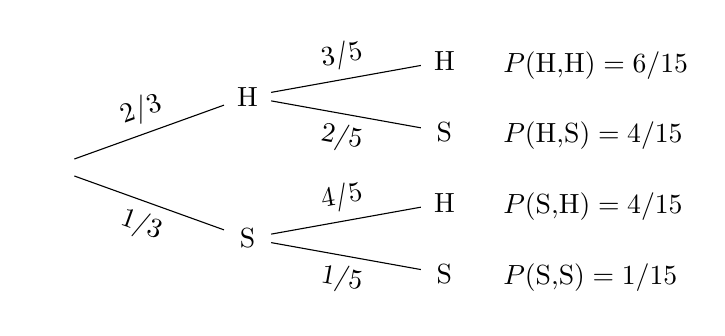
\begin{tikzpicture}[grow=right, sloped]
%wortel
\node[bag] {}
%begin level1-S
    child {
        node[bag] {S}        
%begin level2-SS
        child {
                node[bag] {S}
                node[xshift=0.5cm,yshift=-0.05cm, label=right: {$P($S,S$)=1/15$}] {}
                edge from parent
                node[below=0.0cm] {$1/5$}
                }
%end level2-SS
%begin level2-SH
        child {
                node[bag] {H}
                node[xshift=0.5cm,yshift=-0.05cm, label=right: {$P($S,H$)=4/15$}] {}
                edge from parent
                node[above=0.0cm] {$4/5$}
        }        
%end level2-SH
        edge from parent
        node[below=0.0cm] {$1/3$}
    }
%end level1-S
%begin level1-H
    child {
        node[bag] {H}        
%begin level2-HS
        child {
                node[bag] {S}
                node[xshift=0.5cm,yshift=-0.05cm, label=right: {$P($H,S$)=4/15$}] {}
                edge from parent
                node[below=0.0cm] {$2/5$}
           }
%end level2-HS
%begin level2-HH
        child {
                node[bag] {H}
                node[xshift=0.5cm,yshift=-0.05cm, label=right: {$P($H,H$)=6/15$}] {}
                edge from parent
                node[above=0.0cm] {$3/5$}
           }
%end level2-HH
        edge from parent
        node[above=0.0cm] {$2/3$}
    };
%end level1-H
%end wortel
\end{tikzpicture}
\caption{Kansboom harten en schoppen}
\label{fig:kaarten_versie04}
\end{afbeeldingenv}
 %einde figuur



 
\subsection*{Kansrekenen met een kansboom - Somregel en productregel}
We gaan verder met het voorbeeld van de kaarten. De volgende vragen los je op door de kansboom te gebruiken.  Hier duiken de product- en somregel op.
\begin{vraagenantwoord} 
\vraag{Wat is de kans om eerst een schoppen kaart en dan een harten kaart te trekken?} 
\antwoord{In deze vraag komt op natuurlijke wijze de productregel aan bod: $P(S,H)=\frac{1}{3}\cdot\frac{4}{5}=\frac{4}{15}\approx27\%.$} 
\vraag{Wat is de kans om als tweede kaart een harten te trekken (dus zonder dat je weet wat de eerste kaart is)? }
\antwoord{Vermits de eerste kaart zowel een harten als schoppen kaart kan zijn moeten we de kansen bij twee bladeren optellen: $P(H,H)+P(S,H)=\frac{2}{3}\cdot\frac{3}{5}+\frac{1}{3}\cdot\frac{4}{5}=\frac{2}{3}\approx67\%.$}

\vraag{Wat is de kans op één schoppen en één harten, ongeacht de volgorde waarin ze getrokken worden? }
\antwoord{We gebruiken de notatie met een verzameling omdat de volgorde niet uitmaakt. We moeten weer de kansen bij twee bladeren optellen. $P\{S,H\}=P(H,S)+P(S,H)=\frac{2}{3}\cdot\frac{2}{5}+\frac{1}{3}\cdot\frac{4}{5}=\frac{8}{15}\approx53\%.$}
\end{vraagenantwoord}

\subsection{Kruistabellen}
\subsection*{Kruistabellen en boomdiagrammen}
We nemen de volgende gegevens uit Delta 5/6 (Arts et al. 2024) in \autoref{mobil}. Via dit voorbeeld laten we de leerlingen kennismaken met een nieuwe manier om dergelijke gegevens voor te stellen, namelijk een kruistabel. 

\end{multicols}
\afbeelding[12cm]{img/3B2Mobil.jpg}{Bedrijf met mobiliteitsformules}{mobil}
\begin{multicols}{2}
 
We vragen eerst om een tabel op te stellen waarin de gegevens voorkomen. Leerlingen die niet kunnen starten geven we de volgende meer gesloten vraag: Welke gegevens kunnen we rechtstreeks uit de opgave afleiden en waar kunnen we die  invullen in de onderstaande tabel? 
\begin{tabel}
\begin{tabular}{m{1.1 cm} C{1.5cm} C{1.5cm} C{1.5cm} C{1cm}}
	\hlinethick
	\tableheader{} & \tableheader{\small{Formule 1}} & \tableheader{\small{Formule 2}} & \tableheader{\small{Formule 3}} & \tableheader{totaal} \\
	\hlinethick
		\small {dichtbij} &  &  & &  \\
		\small veraf & & & & \\
		\small totaal &  & & & \\
	\hlinethick
	\end{tabular}
	\caption{Kruistabel mobilteitsformules bedrijf}
	\end{tabel}
Vervolgens vragen we om ook de andere aantallen te berekenen en de tabel te vervolledigen. Dit geeft de ingevulde kruistabel hieronder uit (Deloddere et al. 2009).
\afbeelding{img/3B3MobiltabA.jpg}{Kruistabel mobiliteitsformules bedrijf}{mobiltabA}
In dit soort tabel worden de relaties tussen verschillende variabelen voorgesteld, in dit geval ‘dichtbij/veraf wonen’ en ‘gekozen mobiliteitsformule’. De rijen tonen de categorieën van de ene variabele en de kolommen die van de andere. De gegevens uit de opgave kan men in deze tabel rechtsreeks invullen. Ze staan ‘centraal’ in de tabel. De kolom en rij op de rand of in de ‘marge’ van de tabel geven de totalen, waarvan we er een aantal ook zullen gebruiken om het boomdiagram op te stellen. We noemen ze ‘marginale frequenties’. Ze volgen heel natuurlijk bij het aanvullen van de kolommen en rijen. Het opstellen van een kruistabel lijkt bij dit soort opgaven eenvoudiger dan een boomdiagram.
In \autoref{fig:woonwerk} tonen we een boomdiagram dat dezelfde gegevens weergeeft. 

Bemerk dat we de getallen nu bij de wortel en de knopen zelf plaatsen, en niet bij de takken. Hoewel het zeker heel nuttig en behulpzaam is om een dergelijk boomdiagram met absolute frequenties te maken, is het noch een kansboom, noch een telboom in de betekenis zoals we deze begrippen hierboven gemaakt hebben. Daarom gebruiken we in dit geval de overkoepelende term boomdiagram. Er is hier geen sprake van een telprobleem. De getallen die bij de bladeren staan, komen helemaal niet tot stand via de productregel.

%begin figuur
\begin{afbeeldingenv}
% Set the overall layout of the tree
\tikzstyle{level 1}=[level distance=2cm, sibling distance=3.3cm]
\tikzstyle{level 2}=[level distance=2.5cm, sibling distance=1.1cm]

% Define styles for bags and leafs
\tikzstyle{bag} = [text width=2em, text centered]

\hspace{1.3cm}woonplaats \hspace{1.0cm}formule \hspace{0.1cm}combinatie
\\
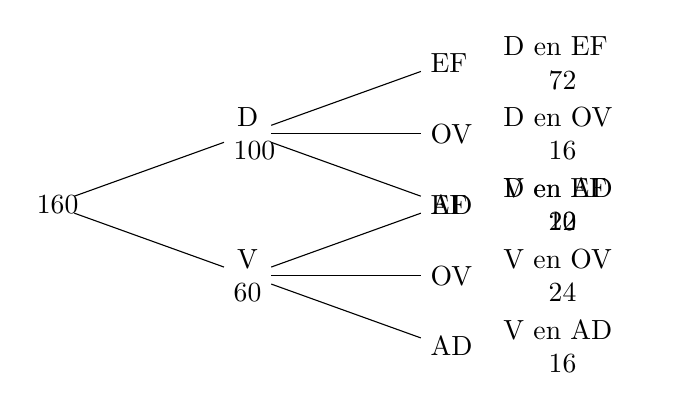
\begin{tikzpicture}[grow=right, sloped]
%wortel
\node[bag] {$160$}
%begin level1-V
    child {
        node[bag] {V 60}        
%begin level2-AD
        child {
                node[bag] {AD}
                node[xshift=1.5cm,yshift=-0.0cm, text width=1.5cm, align=center, label=right: {}] {V en AD \newline $16$}
                edge from parent
                }
%end level2-V-AD
%begin level2-V-OV
        child {
                node[bag] {OV}
                node[xshift=1.5cm,yshift=-0.0cm, text width=1.5cm, align=center, label=right: {}] {V en OV \newline $24$}
                edge from parent
        }        
%end level2-V-OV
%begin level2-V-EF
        child {
                node[bag] {EF}
                node[xshift=1.5cm,yshift=-0.0cm, text width=1.5cm, align=center, label=right: {}] {V en EF \newline $20$}
                edge from parent
        }        
%end level2-V-EF
        edge from parent
    }
%end level1-V
%begin level1-D
    child {
        node[bag] {D 100}        
%begin level2-D-AD
        child {
                node[bag] {AD}
                node[xshift=1.5cm,yshift=-0.0cm, text width=1.5cm, align=center, label=right: {}] {D en AD \newline $12$}
                edge from parent
                }
%end level2-D-AD
%begin level2-D-OV
        child {
                node[bag] {OV}
                node[xshift=1.5cm,yshift=-0.0cm, text width=1.5cm, align=center, label=right: {}] {D en OV \newline $16$}
                edge from parent
        }        
%end level2-D-OV
%begin level2-D-EF
        child {
                node[bag] {EF}
                node[xshift=1.5cm,yshift=-0.0cm, text width=1.5cm, align=center, label=right: {}] {D en EF \newline $72$}
                edge from parent
        }        
%end level2-D-EF
        edge from parent
    };
%end level1-D
%end wortel
\end{tikzpicture}
\caption{Boomdiagram mobiliteitsformules bedrijf}
\label{fig:woonwerk}
\end{afbeeldingenv}
%einde figuur


In het boomdiagram komen (uiteraard) dezelfde twee variabelen aan bod als in de kruistabel, maar de symmetrie wordt doorbroken: de eerste generatie vertakkingen betreft de eigenschap ‘woonplaats’ en de tweede de eigenschap ‘formule’. We vinden in het boomdiagram wèl de marginale frequenties voor ‘woonplaats’ maar niet (rechtstreeks) de marginale frequenties voor ‘formule’.
Uit deze gegevens kan men heel wat andere gegevens afleiden. Om inzicht in het probleem krijgen, zijn de volgende vragen zinvol om te stellen: 
\begin{vraagenantwoord}
    \vraag{Welke soort gegevens lezen we meteen af uit de opgave? Welke gegevens niet?}
    \antwoord{Er zijn drie mobiliteitsformules. Er zijn werknemers die dichtbij en veraf wonen. Zowel van diegene die dichtbij als veraf wonen, kennen we het aantal dat voor elke formule kiest. De totalen voor dichtbij/veraf wonen en voor de formules zijn niet gegeven. We lezen ook niet meteen hoeveel werknemers in het bedrijf werken.}
    \vraag{Stel dat we hier een boomdiagram bij maken. Wat stellen de wortel, de generaties, de knopen en de bladeren voor? }
    \antwoord{Het getal bij de wortel is het totale aantal werknemers. De getallen bij de knopen van de eerste generatie geven aan hoeveel werknemers dichtbij, respectievelijk veraf wonen. De knopen van de tweede generatie stellen de formules voor waarvoor de werknemers kiezen als ze dichtbij dan wel veraf wonen. De bladeren geven de combinatie woonplaats-formule weer. De getallen bij de bladeren stellen het aantal werknemers voor dat overeenkomt met een bepaalde combinatie van woonplaats en formule. Zo zijn er bijvoorbeeld 16 werknemers die dichtbij wonen en kiezen voor het openbaar vervoer.}
    \vraag{Bepaal de informatie die je kunt toevoegen aan het boomdiagram. Hebben we hier te maken met een telboom?}
    \antwoord{Het totaal aantal werknemers dat dichtbij (resp. veraf) woont is $100$ (resp. $60$), het totaal aantal werknemers is dus $160$.}
\end{vraagenantwoord}
    
\subsection*{Absolute frequentie}
Vermits volgens de eindtermen 06.13 (doorstroom) en 06.06 (dubbele finaliteit) relatieve frequentie in verband gebracht moet worden met kansen, kan het geen kwaad om bij het aanbrengen van kruistabellen te spreken over absolute frequentie. In de tabel staan immers absolute frequenties. De getallen in de opgave geven allemaal aan hoe vaak een bepaalde gebeurtenis (dichtbij/veraf wonen en een bepaalde formule kiezen) voorkomt in een dataset van het mobiliteitsonderzoek in het bedrijf.
\subsection*{Kansen berekenen met een kruistabel}
We grijpen terug naar het voorbeeld van de werknemers en maken er nu een kansprobleem van. We kiezen lukraak een van de werknemers.  We hebben bijvoorbeeld de namen van elk van de 160 werknemers op een briefje geschreven en die 160 briefjes stoppen we in een ton. We laten een onschuldige hand hieruit lukraak één briefje trekken.
\begin{vraagenantwoord}
    \vraag{Wat is de kans dat de gekozen werknemer iemand zal zijn die voor formule 2 gekozen heeft?}
    \antwoord{Dankzij de wet van Laplace vinden we deze kans: deel het aantal werknemers dat voor formule 2 gekozen heeft ($40$) door het totale aantal werknemers ($160$):  $\frac{40}{160}=25\%$. We maken hier dus gebruik van een van de marginale frequenties.}
    \vraag{Wat is de kans dat de gekozen werknemer iemand zal zijn die dichtbij woont en voor formule 2 gekozen heeft. }
    \antwoord{We vinden deze kans op een gelijkaardige manier als bij vraag $1$, maar nu moeten we gebruik maken van een van de frequenties uit de middelste cellen: $16$ werknemers wonen dichtbij en kozen bovendien voor formule 2. In de noemer vinden we nog altijd het totale aantal werknemers. De kans om lukraak zo’n werknemer te trekken, is dus $\frac{16}{160}=10\%$.}
    \vraag{Wat is de kans dat een werknemer die voor formule 2 gekozen heeft dichtbij woont? }
    \antwoord{We moeten in de noemer nu niet met het totale aantal werknemers werken, maar met het aantal werknemers dat voor formule $2$ gekozen heeft ($40$). Binnen die groep tellen we dan hoeveel er voor formule $2$ gekozen hebben ($16$). De kans is dus $\frac{16}{40}=40\%$.}
    Bemerk verder het onderscheid tussen de drie situaties
    \begin{itemize}
        \item in de eerste vraag zijn we geïnteresseerd in werknemers die aan één eigenschap voldoen;
        \item in de tweede vraag kijken we naar werknemers die tegelijk aan twee eigenschappen voldoen;
        \item in de derde vraag kijken we naar werknemers waarvan we reeds weten dat ze de ene eigenschap hebben en vragen we ons af wat dan de kans is dat ze ook de tweede eigenschap hebben.
    \end{itemize}
In de volgende vraag doet de somregel in een kruistabel zich voor.
    \vraag{Wat is de kans dat een werknemer veraf woont of voor formule 1 koos. }
    \antwoord{We berekenen eerst het aantal werknemers dat veraf woont of voor formule $1$ koos. Hiervoor moeten we aantallen in meerdere cellen optellen. We vinden deze werknemers in de cel ‘dichtbij én formule $1$’ ($72$), ‘veraf en formule $1$’ ($20$), ‘veraf en formule $2$’ ($24$) en ‘veraf en formule $3$’ ($16$). Het kan ook korter door de laatste drie aantallen te vervangen door de marginale frequentie ‘veraf’ ($60$). Dit zou je de somregel voor kruistabellen kunnen noemen. Om de gevraagde kans te vinden, moeten we tot slot delen door het totale aantal (160): $\frac{72+20+24+16}{160}=\frac{72+60}{160}=\frac{132}{160}=82,5\%$.}
\end{vraagenantwoord}

\subsection*{Een kruistabel met kansen (of relatieve frequenties)}
In het voorbeeld van de werknemers vertrokken we van een kruistabel met aantallen, maar we kunnen ook een tabel met de kansen opstellen, zoals in de \autoref{mobilP} hieronder. We herkennen de kansen die we hierboven berekend hebben bij vraag 1 en 2 (0,25 en 0,1). De andere kansen worden analoog berekend. In dit geval (lukraak kiezen uit alle werknemers) zijn de kansen gewoon relatieve frequenties omdat we de kansen bereken door de aantallen in elke cel te delen door het totale aantal werknemers. 
\afbeelding{img/3BMobiltabP.jpg}{Kruistabel mobiliteitsformules bedrijf}{mobilP}
De kansen die we berekenden bij vraag 3 en 4 vinden we niet rechtstreeks in de tabel terug. We kunnen ze echter wel berekenen aan de hand van deze kruistabel, zonder dat we terug hoeven te gaan naar de kruistabel met de absolute aantallen. 

Voor het antwoord op vraag 3 kunnen we dat eenvoudig inzien als we in de berekening de teller en noemer delen door 160: $\frac{16}{40}=\frac{\frac{16}{160}}{\frac{40}{160}}=\frac{0,1}{0,25}$.

Voor het antwoord op vraag 4 tellen we de kans dat een werknemer dichtbij woont en voor formule 1 koos op bij de kans dat hij veraf woont $0,45+0,375=82,5\%$. We vinden deze kansen in de tabel op het kruispunt van dichtbij en formule 1 en als marginale kans in de randkolom.

Het is voor leerlingen niet altijd eenvoudig om uit de formulering de correcte kans af te leiden. Het maken van een aantal vertaaloefeningen is dus zeker aangewezen. In de volgende vragen zit het verschil soms in één woord. Deze opgaven tonen het belang van taal binnen dit onderdeel van wiskunde. De vragen gaan allemaal over de eigenschappen ‘veraf wonen’ en ‘formule 1 kiezen’.
\begin{vraagenantwoord}
    \vraag{Wat is de kans dat een werknemer veraf woont en voor formule 1 koos?}
    \antwoord{We moeten de kans bepalen dat twee eigenschappen tegelijk van toepassing zijn. Deze kansen vinden we in het centrale gedeelte van de kruistabel. Het antwoord $0,125=12,5\%$ vinden we in de tabel op het kruispunt van veraf en formule $1$.}
    \vraag{Wat is de kans dat een werknemer die veraf woont voor formule 1 koos?}
    \antwoord{De situatie is nu anders dan bij de vorige vraag. We beperken onze blik tot de werknemers die veraf wonen en onderzoeken hoe groot de kans is dat zo’n werknemer voor formule $1$ koos. Het antwoord is  $\frac{0,125}{0,375}=33,33\%$. Als leerlingen moeite hebben om dit te begrijpen, kun je opnieuw een redenering geven die het verband tussen de tabellen met absolute en relatieve frequenties toont. Het aantal werknemer dat veraf woont, is $60$. Van deze werknemers kozen er $20$ voor formule $1$. De berekening wordt dan: $\frac{20}{60}=\frac{\frac{20}{160}}{\frac{60}{160}}=\frac{0,125}{0,375}$.}
    \vraag{Wat is de kans dat een werknemer die koos voor formule 1 ook veraf woont? }
    \antwoord{In deze vraag gaat het over dezelfde eigenschappen als in de vorige vraag, maar hun rol is omgewisseld. We beperken onze blik tot werknemers die voor formule $1$ kozen en onderzoeken hoe groot de kans is dat zo’n werknemer veraf woont. Het antwoord is $\frac{0,125}{0,575} =21,74\%$. We delen de kans dat een werknemer koos voor formule $1$ en veraf woont door de kans dat een werknemer voor formule $1$ koos.}   
\end{vraagenantwoord}

\subsection*{Van kruistabel naar kansboom}
We keren nog even terug naar het boomdiagram uit \autoref{fig:woonwerk}, dat geen telboom en ook geen kansboom was. In de figuur hieronder hebben we het boomdiagram aangevuld met kansen langs de takken. Sommige van deze kansen vind je rechtstreeks terug in de kruistabel, maar voor andere moet je eerst nog een berekening maken. We hebben ook aangegeven hoe de aantallen die er oorspronkelijk in stonden en de kansen die we nu toegevoegd hebben aan elkaar gerelateerd zijn. We hebben nu wel degelijk een kansboom, die aangevuld of uitgebreid is met aantallen. We zouden dit boomdiagram bijvoorbeeld een ‘uitgebreide kansboom’ kunnen noemen.

\end{multicols}

%begin figuur
\begin{afbeeldingenv}
% Set the overall layout of the tree
\tikzstyle{level 1}=[level distance=2.5cm, sibling distance=2.4cm]
\tikzstyle{level 2}=[level distance=3cm, sibling distance=0.8cm]

% Define styles for bags and leafs
\tikzstyle{bag1} = [text width=5em, text centered]
\tikzstyle{bag2} = [text width=2em, text centered]

\hspace{-3.0cm}woonplaats \hspace{1.5cm}formule \hspace{0.0cm}combinatie
\\
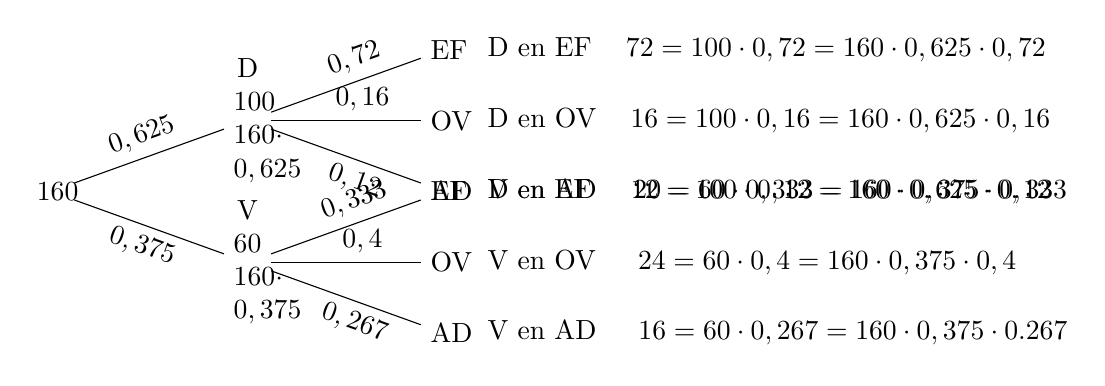
\begin{tikzpicture}[grow=right, sloped]
%wortel
\node[bag1] {$160$}
%begin level1-V
    child {
        node[bag1] {V \\60 $160\cdot0,375$}        
%begin level2-AD
        child {
                node[bag2] {AD}
                node[xshift=0.3cm,yshift=-0.0cm, label=right: V en AD \hspace{0.3cm} {$16=60\cdot0,267=160\cdot0,375\cdot0.267$}] {}
                edge from parent
                node[below=0.0cm] {\hspace{0.3cm} $0,267$}
                }
%end level2-V-AD
%begin level2-V-OV
        child {
                node[bag2] {OV}
                node[xshift=0.3cm,yshift=-0.0cm, label=right: {V en OV \hspace{0.3cm} $24=60\cdot0,4=160\cdot0,375\cdot0,4$}] {}
                edge from parent
                node[above=0.0cm] {\hspace{0.3cm} $0,4$}
        }        
%end level2-V-OV
%begin level2-V-EF
        child {
                node[bag2] {EF}
                node[xshift=0.3cm,yshift=-0.0cm, label=right: {V en EF \hspace{0.3cm} $20=60\cdot0,333=160\cdot0,375\cdot0,333$} ] {}
                edge from parent
                node[above=0.0cm] {\hspace{0.3cm} $0,333$}
        }        
%end level2-V-EF
        edge from parent
        node[below=0.0cm] {$0,375$}
    }
%end level1-V
%begin level1-D
    child {
        node[bag1] {D \\100 $160\cdot0,625$}        
%begin level2-D-AD
        child {
                node[bag2] {AD}
                node[xshift=0.3cm,yshift=-0.0cm, label=right: {D en AD \hspace{0.2cm} $12=100\cdot0,12=160\cdot0,625\cdot0,12$}] {}
                edge from parent
                node[below=0.0cm] {\hspace{0.3cm} $0,12$}
                }
%end level2-D-AD
%begin level2-D-OV
        child {
                node[bag2] {OV}
                node[xshift=0.3cm,yshift=-0.0cm, label=right: {D en OV \hspace{0.2cm} $16=100\cdot0,16=160\cdot0,625\cdot0,16$}] {}
                edge from parent
                node[above=0.0cm] {\hspace{0.3cm} $0,16$}
        }        
%end level2-D-OV
%begin level2-D-EF
        child {
                node[bag2] {EF}
                node[xshift=0.3cm,yshift=-0.0cm, label=right: {D en EF \hspace{0.2cm} $72=100\cdot0,72=160\cdot0,625\cdot0,72$}] {}
                edge from parent
                node[above=0.0cm] {\hspace{0.3cm} $0,72$}
        }        
%end level2-D-EF
        edge from parent
        node[above=0.0cm] {$0,625$}
    };
%end level1-D
%end wortel
\end{tikzpicture}
\caption{Boomdiagram mobiliteitsformules bedrijf met kansen}
\label{fig:woonwerk_kansen}
\end{afbeeldingenv}
%einde figuur

\begin{multicols} {2}

\subsection*{Van kansboom naar kruistabel}
Als we een situatie in een kansboom kunnen voorstellen, dan kunnen we ze ook in een kruistabel voorstellen. We illustreren dit met het voorbeeld van het trekken van twee kaarten uit paragraaf 3.3 en \autoref{fig:kaarten_versie04} uit paragraaf 4.1.

Net zoals in de kansboom zijn er twee eigenschappen of variabelen die van belang zijn: de soort van de eerst getrokken kaart en de soort van de tweede kaart die getrokken wordt. In de kruistabel hieronder hebben we in de eerste kolom de mogelijkheden geplaatst voor de eerste kaart en vinden we in de bovenste rij dan de mogelijkheden voor de tweede kaart, maar je mag de twee ook omwisselen (en je mag ‘schoppen’ en ‘harten natuurlijk ook omwisselen). In de middelste cellen van de kruistabel vullen we de kansen van de bladeren van de kansboom in. De marginale kansen in de laatste kolom vinden we door de kansen in de rijen op te tellen, maar we vinden ze ook terug in de kansboom. De marginale kansen in de onderste rij vinden we door de kansen in de kolommen op te tellen. Deze marginale kansen vinden we echter niet onmiddellijk terug in de kansboom. In het vak rechtsonder vullen we uiteraard 1 in.


\begin{tabel}
\begin{tabular}{m{1.5cm} C{1.8cm} C{1.8cm} C{1.1cm}}
	\hlinethick
	\tableheader{} & \tableheader{\small 2de kaart harten} & \tableheader{2de kaart schoppen} & \tableheader{totaal} \\
	\hlinethick
		1ste kaart schoppen & $\frac{6}{15}$ & $\frac{4}{15}$ & $\frac{2}{3}$ \\
		1ste kaart harten  & $\frac{4}{15}$ & $\frac{1}{15}$ & $\frac{1}{3}$ \\
        totaal & $\frac{2}{3}$  & $\frac{1}{3}$ & $1$ \\
	\hlinethick
	\end{tabular}
	\caption{Kruistabel bij het kansexperiment over het trekken van 2 kaarten uit een onvolledige set van 15 kaarten}
    \label{tab:kaartvb15}
	\end{tabel}

Als we de kansen van de bladeren van de kansboom nog niet berekend hebben, kunnen we licht anders tewerk gaan. We gaan dan van links naar rechts in de kansboom en vullen eerst de marginale kansen in de laatste kolom in. Vervolgens gebruiken we de kansen langs de takken van de tweede generatie om daarmee de kansen in het centrale gedeelte van de kruistabel te berekenen (wat natuurlijk neerkomt op het berekenen van de kansen van de bladeren).


\section{Kansrekenen met kansbomen, kruistabellen en aantallen}
Voor de aanpak van het volgende voorbeeld, dat we overnamen uit een toelatingsexamen geneeskunde (Copilot), hebben we ons geïnspireerd op het spinnenweb in Uitwiskeling 18/4 ‘Bayes in kansbomen’ (Tytgat 2002).
Een ziekenhuis onderzoekt de effectiviteit van drie verschillende behandelingen (X, Y en Z) voor een bepaalde chronische aandoening. De kansen op herstel na elke behandeling zijn als volgt:
\begin{itemize}
    \item De kans op herstel na behandeling X is 0,7;
    \item De kans op herstel na behandeling Y is 0,5;
    \item De kans op herstel na behandeling Z is 0,4.
\end{itemize}
De kans dat een patiënt behandeling X krijgt is 0,35, behandeling Y is 0,4 en behandeling Z is 0,25.
Vraag: Wat is de kans dat een patiënt behandeling X heeft gekregen, gegeven dat hij hersteld is?

Omdat het redeneren met absolute aantallen verhelderend kan zijn voor leerlingen, vullen we de kansboom aan tot een uitgebreide kansboom. We vertrekken bijvoorbeeld met 1000 patiënten bij de wortel. De uitgebreide kansboom geeft weer wat er ‘idealiter’ zou gebeuren met deze 1000 patiënten. Het is geen zuivere kansboom omdat de aantallen in de knopen niet bij een kansboom horen en omdat er niet echt sprake is van een kansexperiment.


%begin figuur
% Set the overall layout of the tree
\tikzstyle{level 1}=[level distance=2cm, sibling distance=2.2cm]
\tikzstyle{level 2}=[level distance=2.5cm, sibling distance=1.1cm]

% Define styles for bags and leafs
\tikzstyle{bag} = [text width=2em, text centered]

%hier puzzeken zodat de tekst nog hoort bij volgende figuur




\hspace{1.5cm}behandeling \hspace{0.9cm}herstel? \hspace{0.0cm}combinatie
\begin{afbeeldingenv}
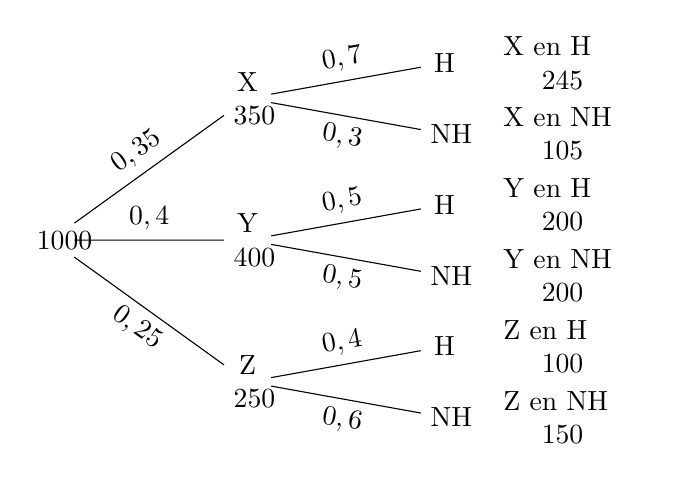
\begin{tikzpicture}[grow=right, sloped]
%wortel
\node[bag] {$1000$}
%begin level1-Z
    child {
        node[bag] {Z 250}        
%begin level2-Z-NH
        child {
                node[bag] {NH}
                node[xshift=1.5cm,yshift=-0.0cm, text width=1.5cm, align=center, label=right: {}] {Z en NH \newline $150$}
                edge from parent
                node[below=0.0cm] {$0,6$}
                }
%end level2-Z-NH
%begin level2-Z-H
        child {
                node[bag] {H}
                node[xshift=1.5cm,yshift=-0.0cm, text width=1.5cm, align=center, label=right: {}] {Z en H \newline $100$}
                edge from parent
                node[above=0.0cm] {$0,4$}
                }
%end level2-Z-NH
        edge from parent
        node[below=0.0cm] {$0,25$}
    }
%end level1-Z
%begin level1-Y
    child {
        node[bag] {Y 400}        
%begin level2-Y-NH
        child {
                node[bag] {NH}
                node[xshift=1.5cm,yshift=-0.0cm, text width=1.5cm, align=center, label=right: {}] {Y en NH \newline $200$}
                edge from parent
                node[below=0.0cm] {$0,5$}
                }
%end level2-Y-NH
%begin level2-Y-H
        child {
                node[bag] {H}
                node[xshift=1.5cm,yshift=-0.0cm, text width=1.5cm, align=center, label=right: {}] {Y en H \newline $200$}
                edge from parent
                node[above=0.0cm] {$0,5$}
                }
%end level2-Y-NH
        edge from parent
        node[above=0.0cm] {$0,4$}
    }
%end level1-Y
%begin level1-X
    child {
        node[bag] {X 350}        
%begin level2-X-NH
        child {
                node[bag] {NH}
                node[xshift=1.5cm,yshift=-0.0cm, text width=1.5cm, align=center, label=right: {}] {X en NH \newline $105$}
                edge from parent
                node[below=0.0cm] {$0,3$}
                }
%end level2-X-NH
%begin level2-X-H
        child {
                node[bag] {H}
                node[xshift=1.5cm,yshift=-0.0cm, text width=1.5cm, align=center, label=right: {}] {X en H \newline $245$}
                edge from parent
                node[above=0.0cm] {$0,7$}
                }
%end level2-X-NH
        edge from parent
        node[above=0.0cm] {$0,35$}
    };
%end level1-X
%end wortel
\end{tikzpicture}
\caption{Uitgebreide kansboom met aantallen - Kans op herstel na een behandeling}
\label{fig:3behandelingen}
\end{afbeeldingenv}

%einde figuur

Met behulp van deze uitgebreide kansboom kun je de volgende vragen oplossen (de tweede vraag is deze van het toelatingsexamen).
\begin{vraagenantwoord}
    \vraag{Wat is de kans op herstel? }
    \antwoord{We tellen hiervoor het totaal aantal patiënten dat herstelde en delen het door het totaal aantal patiënten:$\frac{245+200+100}{1000}=0,545=54,5\%$}
    \vraag{Wat is de kans dat een patiënt behandeling X heeft gekregen, gegeven dat hij hersteld is?}
    \antwoord{Er zijn $545$ patiënten die herstelden en daarvan kregen $245$ patiënten een behandeling X. We vinden dus $\frac{245}{545}=0,4495\approx45\%$.}
\end{vraagenantwoord}
We kunnen hetzelfde probleem ook in de vorm van een kruistabel voorstellen. We hebben de keuze tussen de (fictieve) aantallen en de percentages. Hieronder vind je in \autoref{tab:behandelingA} en \autoref{tab:behandelingP} beide versies. Het is duidelijk dat de tabel met aantallen heel wat minder abstract is dan diegene met de percentages. De gekleurde percentages stellen de gegevens voor en tonen hoe je die tabel opbouwt vanuit de gegevens. In beide tabellen vullen we eerst de onderste rij in. Vervolgens berekenen we de getallen in de tweede rij. De derde rij vullen we als laatste in. In de tweede rij van de onderste tabel vinden we de percentages als resultaten van de productregel bij de bijhorende kansboom die je vindt in \autoref{fig:3behandelingen}.

In \autoref{fig:3behandelingen_kansen} merk je weer dat de kansen uit het centrale deel en de onderste rij van de kruistabel te vinden zijn in de kansboom. 

\end{multicols}
\vspace{1cm}
\definecolor{oranje}{RGB}{255,165,0}
\definecolor{groen}{RGB}{0,128,0}
\definecolor{lichtgroen}{RGB}{144,238,144}
\begin{tabel}
\begin{tabular}{m{1.8 cm} C{2.8cm} C{2.8cm} C{2.8cm} C{3.7cm}}
	\hlinethick
	\tableheader{} & \tableheader{X} & \tableheader{Y} & \tableheader{Z} & \tableheader{totaal} \\
	\hlinethick
		herstelt &$350\cdot{\color{oranje}0,7}=245$ & $400\cdot{\color{oranje}0,5}=200$ & $250\cdot{\color{oranje}0,4}=100$ & $245+200+100=545$\\
		herstelt niet & $350-245=105$&$400-200=200$ &$250-100=150$ &$105+200+150=455$ \\
		totaal &$1000\cdot{\color{lichtgroen}0,35}=350$  &$1000\cdot{\color{lichtgroen}0,4}=400$ & $1000\cdot{\color{lichtgroen}0,25}=250$ &1000 \\
	\hlinethick
	\end{tabular}
	\caption{Kruistabel effectiviteit behandeling in ziekenhuis met absolute frequenties}\label{tab:behandelingA}
	\end{tabel}
\begin{tabel}

\vspace{1cm}

\begin{tabular}{m{1.8 cm} C{2.8cm} C{2.8cm} C{2.8cm} C{3.7cm}}
	\hlinethick
	\tableheader{} & \tableheader{X} & \tableheader{Y} & \tableheader{Z} & \tableheader{totaal} \\
	\hlinethick
		herstelt &${\color{lichtgroen}0,35}\cdot{\color{oranje}0,7}=0,245$ & ${\color{lichtgroen}0,4}\cdot{\color{oranje}0,5}=0,2$ & ${\color{lichtgroen}0,25}\cdot{\color{oranje}0,4}=0,1$ & $0,245+0,2+0,1=0,545$\\
		herstelt niet & ${\color{lichtgroen}0,35}\cdot{\color{oranje}0,3}=0,105$&${\color{lichtgroen}0,4}\cdot{\color{oranje}0,5}=0,2$ &${\color{lichtgroen}0,25}\cdot{\color{oranje}0,6}=0,15$ &$0,105+0,2+0,15=0,455$ \\
		totaal &${\color{lichtgroen}0,35}$  &${\color{lichtgroen}0,4}$ & ${\color{lichtgroen}0,25}$ &1 \\
	\hlinethick
	\end{tabular}
	\caption{Kruistabel effectiviteit behandeling in ziekenhuis met relatieve frequenties}\label{tab:behandelingP}
	\end{tabel}

\begin{multicols} {2}

 
%begin figuur
% Set the overall layout of the tree
\tikzstyle{level 1}=[level distance=1.6cm, sibling distance=1.6cm]
\tikzstyle{level 2}=[level distance=2cm, sibling distance=0.8cm]

% Define styles for bags and leafs
\tikzstyle{bag} = [text width=1em, text centered]

\hspace{0.8cm}behandeling \hspace{0.6cm}herstel? \hspace{0.2cm}kans
\begin{afbeeldingenv}
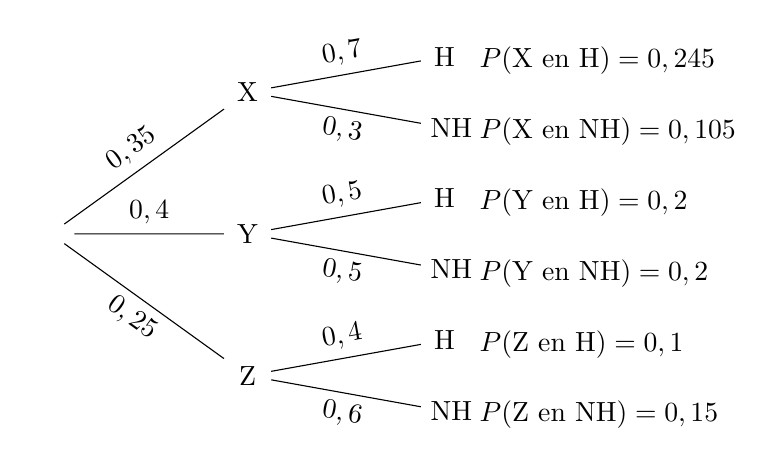
\begin{tikzpicture}[grow=right, sloped]
%wortel
\node[bag] {}
%begin level1-Z
    child {
        node[bag] {Z}        
%begin level2-Z-NH
        child {
                node[bag] {NH}
                node[xshift=0.2cm,yshift=-0.05cm, label=right: {$P($Z en NH$)=0,15$}] {}
                edge from parent
                node[below=0.0cm] {$0,6$}
                }
%end level2-Z-NH
%begin level2-Z-H
        child {
                node[bag] {H}
                node[xshift=0.2cm,yshift=-0.05cm, label=right: {$P($Z en H$)=0,1$}] {}
                edge from parent
                node[above=0.0cm] {$0,4$}
                }
%end level2-Z-NH
        edge from parent
        node[below=0.0cm] {$0,25$}
    }
%end level1-Z
%begin level1-Y
    child {
        node[bag] {Y}        
%begin level2-Y-NH
        child {
                node[bag] {NH}
                node[xshift=0.2cm,yshift=-0.05cm, label=right: {$P($Y en NH$)=0,2$}] {}
                edge from parent
                node[below=0.0cm] {$0,5$}
                }
%end level2-Y-NH
%begin level2-Y-H
        child {
                node[bag] {H}
                node[xshift=0.2cm,yshift=-0.05cm, label=right: {$P($Y en H$)=0,2$}] {}
                edge from parent
                node[above=0.0cm] {$0,5$}
                }
%end level2-Y-NH
        edge from parent
        node[above=0.0cm] {$0,4$}
    }
%end level1-Y
%begin level1-X
    child {
        node[bag] {X}        
%begin level2-X-NH
        child {
                node[bag] {NH}
                node[xshift=0.2cm,yshift=-0.05cm, label=right: {$P($X en NH$)=0,105$}] {}
                edge from parent
                node[below=0.0cm] {$0,3$}
                }
%end level2-X-NH
%begin level2-X-H
        child {
                node[bag] {H}
                node[xshift=0.2cm,yshift=-0.05cm, label=right: {$P($X en H$)=0,245$}] {}
                edge from parent
                node[above=0.0cm] {$0,7$}
                }
%end level2-X-NH
        edge from parent
        node[above=0.0cm] {$0,35$}
    };
%end level1-X
%end wortel
\end{tikzpicture}
\caption{Kansboom - Kans op herstel na een behandeling}
\label{fig:3behandelingen_kansen}
\end{afbeeldingenv}
%einde figuur
We beantwoorden nu de bovenstaande twee vragen opnieuw, maar maken dit keer gebruik van de kruistabel. Het antwoord op vraag 1 lees je meteen af in de kruistabel met de relatieve frequenties in de kolom op de rand: 0,545. 

Voor het antwoord op vraag 2 delen we het percentage patiënten dat een behandeling X kreeg en bovendien herstelden door het percentage herstelde patiënten: $\frac{0,245}{0,545}=0,45$. In de tabel lezen we het percentage van de teller in het centrale gedeelte en de noemer in de randen (een marginale kans). Om deze vraag met de kansboom op te lossen, moeten we om de noemer te vinden de somregel toepassen om zo het percentage van herstelde patiënten te vinden. We tellen alle percentages bij de bladeren die hersteld weergeven op: $0,245+0,2+0,1$. Dit is uiteraard ook de som van de getallen in rij 2 van de kruistabel met percentages. 

\section{Kruistabellen en kansbomen in de maatschappij}
Onderzoeken geven vaak resultaten in absolute of relatieve frequenties die overzichtelijk kunnen weergegeven worden in kruistabellen of kansbomen. We halen enkele interessante thema’s aan om in de klas te behandelen. We behandelen drie thema’s: kleurenblindheid, vals positieven en genetica van ons bloed.
\subsection{Kleurenblindheid}
Zelf leerden we uit een handboek dat kleurenblindheid vaker voorkomt bij jongens dan bij meisjes. Bij het maken van de oefeningen in de klas, bleek verrassend genoeg (of juist niet) dat in zowat elke klas kleurenblinde jongens zaten. 
De tabel in \autoref{kleurblind} komt uit een handboek van Delta (Arts et al. 2024). De kruistabel geeft absolute frequenties bij de variabelen ‘kleurenblind’ en ‘geslacht’ weer. Het handboek vermeldt niet of deze cijfers al dan niet uit een onderzoek komen. Ze kloppen echter wel vrij goed met de realiteit. Wereldwijd zijn 8\% van de mannen kleurenblind en 0,5\% van de vrouwen (Vision center 10/11/2024). Deze twee percentages noemt men prevalentie, een term die gebruikt wordt in de geneeskunde en epidemiologie om aan te geven hoe vaak een bepaalde ziekte of aandoening voorkomt in een specifieke groep mensen op een bepaald moment. We weten ook dat er wereldwijd meer jongens (ongeveer 50,4\%) zijn dan meisjes. In de tabel hieronder heeft men deze verhouding tussen aantal jongens en meisjes niet weerhouden. 
\afbeelding{img/3Dkleurenblind.jpg}{Kleurenblindheid bij jongens en meisjes}{kleurblind}
Als je een oefening wil maken in deze maatschappelijk relevante context, zou je bijvoorbeeld kunnen vragen om een kansboom op te stellen op basis van deze kruistabel of om de kruistabel met relatieve frequenties op te stellen. Je kunt de kansboom aanvullen met de absolute aantallen uit de kruistabel en er dus een uitgebreide kansboom van maken. Dit maakt het concreter voor de leerlingen.
Naast het beantwoorden van vragen zoals in paragraaf 5, kun je leerlingen zelf vergelijkbare vragen laten opstellen. Bijvoorbeeld:
\begin{itemize}
    \item Wat is de kans dat een willekeurige persoon kleurenblind is? 
    \item Wat is de kans dat een willekeurige persoon een jongen is? 
    \item Wat is de kans dat een persoon een jongen is gegeven het feit dat er kleurenblindheid wordt vastgesteld?
    \item Wat is de kans dat een persoon kleurenblind is als het een meisje is?
\end{itemize}

\subsection{Vals positieven}
\label{par:valspos}
We hebben in Uitwiskeling al eerder geschreven over valse positieven o.a. in een loep over besmettingsziekten (Moons et al. 2020) en een spinnenweb over drie representaties van een probleem (Deprez, 2017). Een vals-positief resultaat treedt op wanneer een test aangeeft dat een bepaalde eigenschap aanwezig is, terwijl dat in werkelijkheid niet zo is. Stel je voor dat je een test hebt die controleert of een lamp werkt. Als de test zegt dat de lamp werkt (positief resultaat), maar de lamp is eigenlijk kapot, dan is dat een vals positief resultaat. De test geeft een positief signaal, maar de werkelijkheid is anders. 

In deze paragraaf zoomen we in op medische tests. Als  zwangerschapstest positief aangeeft terwijl de persoon niet zwanger is, heb je een vals positief resultaat. Andere situaties waar je aan kunt denken, zijn een covid-test of een dopingtest. In beide eerder genoemde artikels kun je inspiratie vinden voor relevante en realistische vragen bij deze thema’s. Er komen kruistabellen en kansbomen aan bod en de begrippen sensitiviteit en specificiteit, die belangrijk zijn in het kader van besmettingsziekten, worden toegelicht.

In deze loep geven we een ander thema binnen dezelfde context, namelijk borstkanker. We vonden de opgave in \autoref{borst} in het handboek Delta Nova (Deloddere et al. 2009). Het kan een beladen thema zijn gezien heel wat jongeren geconfronteerd worden met familieleden, vrienden of kennissen die worstelen met een vorm van kanker. Hierop ben je best voorbereid door de context van je leerlingen te kennen. We bespreken vals-positieven en ideeën uit deze loep binnen de context van dit thema. 

\afbeelding{img/3Dborst.jpg}{Opgave over borstkanker}{borst}
In de opgave vinden we de variabelen ‘borstkanker’ en ‘resultaat test’. 
De 2\% in de tekst noemen we volgens het vakjargon ‘de prevalentie’: het percentage besmette personen in een populatie. De populatie die hier vermeld wordt, zijn de vrouwen tussen 40 en 50 jaar. Deze prevalentie van 2\% is een schatting. Ze gaat er bijvoorbeeld van uit dat je alle vrouwen tussen 40 en 50 jaar zou screenen, wat in de praktijk niet het geval is. Men kan dit percentage nooit exact kennen, ook al roept men jaarlijks op tot een bevolkingsscreening. 
De 90\% noemen we ‘de sensitiviteit’: dit percentage drukt uit hoeveel procent vrouwen met borstkanker positief test.
Uit de 5\% in de opgave vinden we een ‘specificiteit’ van 95\%: dit percentage drukt uit hoeveel procent van de vrouwen zonder borstkanker negatief test.



%kurtprent
\end{multicols}
 \afbeelding [10cm]{tekeningenKurt/test.jpg}{}{} 
\begin{multicols}{2} %

De kans die in de opgave gevraagd wordt, gaat over ‘vals positieven’: de vrouwen die een positief testresultaat krijgen zonder dat ze borstkanker hebben. Zo’n vrouw maakt zich onnodig ongerust.
We kunnen net als in de vorige paragraaf dit probleem voorstellen op 4 manieren: een kansboom, een uitgebreide kansboom, een kruistabel met aantallen of een kruistabel met percentages. Afhankelijk van de noden van je leerlingen kies je voor één of meerdere voorstellingen. Om deze voorstelling te maken vanuit de gegevens, moeten leerlingen vragen oplossen zoals in paragraaf 3.2 en 4.1. We stellen eerst een (uitgebreide) kansboom op. Hieronder vind je enkele vragen die je aan leerlingen kunt aanbieden als ze niet kunnen starten.
\begin{vraagenantwoord}
    \vraag{Kies een gepast aantal vrouwen waarop je gaat redeneren. }
    \antwoord{$1000$ vrouwen is een goed aantal omdat de getallen dan allemaal natuurlijk zijn.}
    \vraag{Bepaal de knopen met hun betekenis. }
    \antwoord{De eerste generatie knopen geeft de eigenschap ‘borstkanker’ en de tweede generatie knopen de eigenschap ‘test’.}
    \vraag{Stel op basis van de gegevens een uitgebreide kansboom op. }
    \antwoord{Uit de gegevens gebruiken we voor de eerste vertakking vanuit de wortel het percentage $2\%$, wat aangeeft dat er $20$ vrouwen van de $1000$ borstkanker hebben en $980$ niet. De tweede generatie knopen gaat over het al dan niet hebben van borstkanker. De $90\%$ uit de opgave noteren we bij de eerste vertakking van de knoop ‘wel borstkanker’. We vinden $18$ vrouwen van de $20$ die positief testen en dus $2$ vrouwen negatief. De $5\%$ uit de opgave noteren we bij de tweede vertakking van de knoop ‘geen borstkanker’. Dit levert $49$ van de $980$ vrouwen die positief testen en $931$ van die vrouwen testen negatief.}
\end{vraagenantwoord}
We hebben met deze vragen alle informatie voor de uitgebreide kansboom (en dus ook voor de kansboom). Je vindt beide versie in de figuren hieronder.

%begin figuur
% Set the overall layout of the tree
\tikzstyle{level 1}=[level distance=2cm, sibling distance=2.2cm]
\tikzstyle{level 2}=[level distance=2cm, sibling distance=1.1cm]

% Define styles for bags and leafs
\tikzstyle{bag0} = [text width=3em, text centered]
\tikzstyle{bag1} = [text width=2em, text centered]
\tikzstyle{bag2} = [text width=1em, text centered]

\begin{afbeeldingenv}
\hspace{1.6cm}kanker? \hspace{0.9cm}test \hspace{0.3cm}combinatie
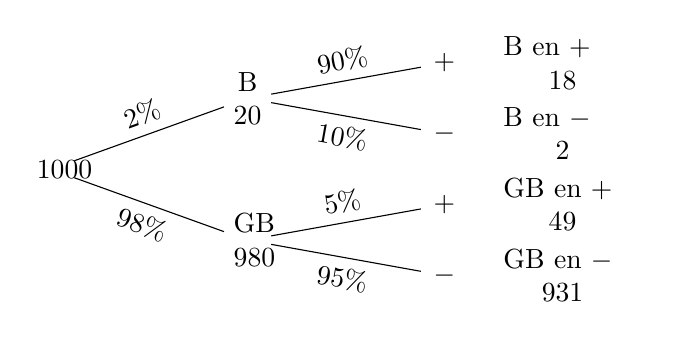
\begin{tikzpicture}[grow=right, sloped]
%wortel
\node[bag0] {1000}
%begin level1-GB
    child {
        node[bag1] {GB \\980}        
%begin level2-GB-
        child {
                node[bag2] {$-$}
                node[xshift=1.5cm,yshift=-0.0cm, text width=1.5cm, align=center, label=right: {}] {GB en $-$ \newline $931$}
                edge from parent
                node[below=0.0cm] {$95\%$}
                }
%end level2-GB-
%begin level2-GB+
        child {
                node[bag2] {+}
                node[xshift=1.5cm,yshift=-0.0cm, text width=1.5cm, align=center, label=right: {}] {GB en $+$ \newline $49$}
                edge from parent
                node[above=0.0cm] {$5\%$}
        }        
%end level2-GB+
        edge from parent
        node[below=0.0cm] {$98\%$}
    }
%end level1-GB
%begin level1-B
    child {
        node[bag1] {B \\20}        
%begin level2-B-
        child {
                node[bag2] {$-$}
                node[xshift=1.5cm,yshift=-0.0cm, text width=1.5cm, align=center, label=right: {}] {B en $-$ \newline $2$}
                edge from parent
                node[below=0.0cm] {$10\%$}
           }
%end level2-B-
%begin level2-B+
        child {
                node[bag2] {+}
                node[xshift=1.5cm,yshift=-0.0cm, text width=1.5cm, align=center, label=right: {}] {B en $+$ \newline $18$}
                edge from parent
                node[above=0.0cm] {$90\%$}
           }
%end level2-B+
        edge from parent
        node[above=0.0cm] {$2\%$}
    };
%end level1-B
%end wortel
\end{tikzpicture}
\caption{Uitgebreide kansboom testen van borstkanker}
\label{fig:kanker_aantallen}
\end{afbeeldingenv}
%einde figuur


%begin figuur
% Set the overall layout of the tree
\tikzstyle{level 1}=[level distance=1.8cm, sibling distance=1.6cm]
\tikzstyle{level 2}=[level distance=1.8cm, sibling distance=0.8cm]

% Define styles for bags and leafs
\tikzstyle{bag0} = [text width=1em, text centered]
\tikzstyle{bag1} = [text width=1em, text centered]
\tikzstyle{bag2} = [text width=1em, text centered]

\begin{afbeeldingenv}
\hspace{0.5cm}kanker? \hspace{0.7cm}test \hspace{0.2cm}combinatie
\\
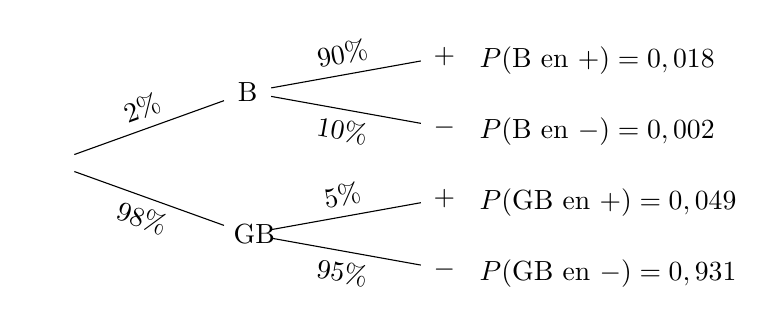
\begin{tikzpicture}[grow=right, sloped]
%wortel
\node[bag0] {}
%begin level1-GB
    child {
        node[bag1] {GB}        
%begin level2-GB-
        child {
                node[bag2] {$-$}
                node[xshift=0.2cm,yshift=-0.05cm, label=right: {$P($GB en $-)=0,931$}] {}
                edge from parent
                node[below=0.0cm] {$95\%$}
                }
%end level2-GB-
%begin level2-GB+
        child {
                node[bag2] {+}
                node[xshift=0.2cm,yshift=-0.05cm, label=right: {$P($GB en $+)=0,049$}] {}
                edge from parent
                node[above=0.0cm] {$5\%$}
        }        
%end level2-GB+
        edge from parent
        node[below=0.0cm] {$98\%$}
    }
%end level1-GB
%begin level1-B
    child {
        node[bag1] {B}        
%begin level2-B-
        child {
                node[bag2] {$-$}
                node[xshift=0.2cm,yshift=-0.05cm, label=right: {$P($B en $-)=0,002$}] {}
                edge from parent
                node[below=0.0cm] {$10\%$}
           }
%end level2-B-
%begin level2-B+
        child {
                node[bag2] {+}
                node[xshift=0.2cm,yshift=-0.05cm, label=right: {$P($B en $+)=0,018$}] {}
                edge from parent
                node[above=0.0cm] {$90\%$}
           }
%end level2-B+
        edge from parent
        node[above=0.0cm] {$2\%$}
    };
%end level1-B
%end wortel
\end{tikzpicture}
\caption{Kansboom testen van borstkanker}
\label{fig:kanker_kansen}
\end{afbeeldingenv}
%einde figuur

Om de kruistabel met absolute frequenties op te stellen hebben we vergelijkbare vragen nodig.
\begin{enumerate}
    \item Welke variabelen komen voor in deze opgave? Zet ze in de eerst rij en kolom van een kruistabel.
    \item Kies het aantal vrouwen waarop je gaat redeneren. Zet het in de cel rechtsonder.
    \item Vul de kruistabel in op basis van de gegevens.
\end{enumerate}
We berekenen op eenzelfde manier als in vraag 3 hierboven eerst de getallen 20 en 980 in de onderste rij, en vervolgens de getallen 18, 2, 49 en 931 in het centrum van de tabel. Tot slot berekenen we de getallen 67 en 933 in de laatste kolom.
\begin{tabel}
\begin{tabular}{m{1.5cm} C{1.8cm} C{1.8cm} C{1.1cm}}
	\hlinethick
	\tableheader{} & \tableheader{B} & \tableheader{GB} & \tableheader{totaal} \\
	\hlinethick
		Test + & $18$ & $49$ & $67$ \\
		Test $-$  & $2$ & $931$ & $933$ \\
        totaal & $20$  & $980$ & $1000$ \\
	\hlinethick
	\end{tabular}
	\caption{Kruistabel bij borstkanker}
	\end{tabel}
De kruistabel met relatieve frequenties kunnen we uit de opgave halen. Doordat elke variabele slechts 2 uitkomsten heeft, geeft de ene uitkomst meteen ook de andere. We moeten daarnaast ook de somregel toepassen. Het is duidelijk dat dit de meest abstracte voorstelling is.
\end{multicols}
\begin{tabel}
\begin{tabular}{m{1.5cm} C{3cm} C{3cm} C{3.8cm}}
	\hlinethick
	\tableheader{} & \tableheader{B} & \tableheader{GB} & \tableheader{totaal} \\
	\hlinethick
		Test + & ${\color{lichtgroen}0,02}\cdot{\color{oranje}0,9}=0,018$ & $0,98\cdot{\color{oranje}0,05}=0,049$ & $0,018+0,049=0,067$ \\
		Test $-$  & ${\color{lichtgroen}0,02}\cdot{\color{oranje}0,1}=0,002$ & $0,98\cdot{\color{oranje}0,95}=0,931$ & $0,002+0,931=0,933$ \\
        totaal & ${\color{lichtgroen}0,02}$  & $0,98$ & $1$ \\
	\hlinethick
	\end{tabular}
	\caption{Kruistabel bij borstkanker}
	\end{tabel}

\begin{multicols}{2}
De vraag in deze opgave: Wat is de kans dat een vrouw met een positief testresultaat daadwerkelijk borstkanker heeft, kunnen we met al deze voorstellingswijzen oplossen op een analoge manier als in paragraaf 5.
\begin{enumerate}
    \item 	A.d.h.v. het boomdiagram of de kruistabel met aantallen berekenen we dit als volgt: Er zijn 18 vrouwen met een positief resultaat en borstkanker. Dit aantal moeten we delen door het totaal aantal vrouwen dat positief test. We krijgen:  $\frac{18}{18+49}=\frac{18}{67} \approx 0,27=27\%$.
    \item 	A.d.h.v. de kansboom of de kruistabel met percentages berekenen we dit als volgt: Er zijn 1,8\% vrouwen met een positief resultaat en borstkanker. Dit percentage moeten we delen door het percentage vrouwen dat positief test (de marginale kans bij Test +). We krijgen:  $\frac{0,018}{0,067} \approx 0,27=27\%$.
\end{enumerate}
Dit resultaat stemt tot nadenken. Slechts 27\% van de vrouwen die positief testen zou dus daadwerkelijk borstkanker hebben. Dit staat in schril contrast met de 90\% sensitiviteit die een gevoel van betrouwbaarheid opwekt. We kunnen ons afvragen wat aan de basis ligt van dit lage percentage. De absolute aantallen helpen ons hierbij. Als we naar de breuk in de berekening hierboven kijken, dan zien we dat er 18 ‘terechte positieven’ zijn en 49 valse positieven. Deze 49 komt tot stand als een relatief klein percentage van een groot aantal vrouwen dat geen borstkanker heeft (980). Dit grote aantal is dan weer het gevolg van de lage prevalentie. Vermits de prevalentie laag is, en er dus relatief gezien weinig vrouwen borstkanker hebben (20), kan zelfs bij een goed ontwikkelde test met een hoge specificiteit zoals hier en dus een laag percentage (5\%) van positieve testen bij vrouwen die geen borstkanker hebben, leiden tot een groot aantal vals positieven (49). De 90\% van de 20 vrouwen met borstkanker die door de test wordt gedetecteerd, zijn dus maar 18 vrouwen van de 67 vrouwen die positief getest worden. In het handboek lezen we verder deze belangrijke boodschap: ‘Dit is een reden waarom vrouwen tussen 40 en 50 niet systematisch worden gescreend. Te veel vrouwen krijgen ten onrechte een positieve test te verwerken en weigeren op latere leeftijd de test opnieuw te ondergaan.’  
    
\subsection{Genetica van ons bloed}
Een laatste maatschappelijke context voor kansrekening die we hier bespreken, is het gebruik van kansbomen in de genetica. Ook daarover schreven we al eerder in een loep over wiskunde en biologie (Verbeeck 2005). In opeenvolgende werkteksten behandelden we kansproblemen over de oorlellen van de nakomelingen van een grootouderpaar waarbij de grootmoeder vaste oorlellen (ll) heeft en de grootvader losse (LL). De l en L staan voor twee varianten, namelijk vast en los, voor de erfelijke eigenschap of het gen dat de vorm van de oorlellen bepaalt. Elk gen bestaat uit 2 allelen afkomstig van de vorige generatie. ll betekent dat zowel de moeder als de vader l doorgaf. We toonden door berekeningen van kansproblemen de wet van Hardy-Weinberg aan die zegt dat \textit{de genenfrequenties en de genotypenfrequenties constant blijven van de ene generatie op de volgende, onder bepaalde voorwaarden}. We schreven ten slotte ook over de genetica van ons bloed. Deze laatste context bekijken we hier opnieuw vanuit het perspectief van deze loep.
\subsection*{De + en $-$ bij bloedgroepen: de rhesusfactor}
We bekijken eerst een kansprobleem over de rhesusfactor. Dit is in feite nog een ander soort bloedgroep (D) dan de gekende A, B, O en AB, maar in de praktijk wordt D nooit vermeld. Iemand met een positieve rhesusfactor ($Rh^+$) heeft antigen D op de rode bloedcellen. De ‘+’ wijst dus op de aanwezigheid van dit antigen. 15,5\% van de Belgische bevolking heeft bloed met rhesusfactor negatief.

Bij bloedtransfusies moet men niet alleen op de bloedgroep, maar ook op de rhesusfactor letten. Als men $Rh^+$-bloed toedient aan iemand die $Rh^-$ is, worden antistoffen gemaakt. Het antigen D wordt immers als lichaamsvreemd ervaren. De eigenschap voor de rhesusfactor wordt bepaald door slechts 2 allelen (zoals bij de losse of vaste oorlellen). We noemen ze R ($Rh^+$) en r ($Rh^-$) omdat $Rh^+$ dominant is over $Rh^-$. 

In het kansexperiment dat we bestuderen, letten we op de allelen voor de rhesusfactor van de nakomeling, met als variabelen ‘het allel voor de rhesusfactor dat door de moeder doorgegeven wordt’ en ‘het allel voor de rhesusfactor dat door de vader doorgegeven wordt’. Er zijn vier uitkomsten, waarbij we eerst het allel van de moeder noteren: RR, Rr, rR en rr. 

Om een kruistabel op te stellen, beschikken we over slechts één percentage namelijk dat 15,5\% van de Belgische bevolking rhesusfactor negatief heeft. Vermits het allel r recessief is, weten we dat dit percentage hoort bij de situatie waarbij zowel vader als moeder het allel r doorgeven. Uit de wet van Hardy-Weinberg volgt dat vader en moeder een gelijke kans hebben om dit allel door te geven, namelijk de kans q die gelijk is aan de relatieve frequentie van dit allel in de populatie. Bijgevolg moet $q^2=0,1550$ en dus $q=\sqrt{0,1550}=0,3937$. 


\end{multicols}
\definecolor{blauw}{RGB}{0,0,255}
\begin{tabel}
\begin{tabular}{m{2.5cm} C{4.2cm} C{4.2cm} C{2.5cm}}
	\hlinethick
	\tableheader{} & \tableheader{allel vader R} & \tableheader{allel vader r} & \tableheader{totaal} \\
	\hlinethick
		allel moeder R & ${\color{blauw}0,6063^2}=0,3676$ & ${\color{oranje}0,3937}\cdot{\color{blauw}0,6063}=0,2387$ & $0,6063$ \\
		allel moeder r  & ${\color{oranje}0,3937}\cdot{\color{blauw}0,6063}=0,2387$ & ${\color{oranje}0,3937^2}=\color{lichtgroen}0,155$ & $0,3937$ \\
        totaal & $1-{\color{oranje}0,3937}={\color{blauw}0,6063}$  & $\color{oranje}0,3937$ & $1$ \\
	\hlinethick
	\end{tabular}
	\caption{Kruistabel allelen rhesusfactor}
\end{tabel}
\begin{multicols}{2}
Het is nu belangrijk om stil te staan bij de interpretatie van de kansen in de tabel. We hebben de getallen in de tabel tot nu toe opgevat als de kans dat de nakomeling van een bepaald genotype (bijvoorbeeld: RR) is. De wet van Hardy-Weinberg zegt echter dat de relatieve frequenties van de allelen en van de genotypes constant blijven. De kansen die we berekend hebben, zijn dus niet enkel van toepassing voor deze ene nakomeling, maar voor een willekeurig individu in de populatie. Het is belangrijk om dit te beseffen voor het beantwoorden van de vraag in de volgende alinea.
Wanneer een zwangere vrouw rhesusnegatief is en haar partner rhesuspositief, dan kan hun kind rhesuspositief bloed hebben. Dit houdt een gevaar in voor een volgende zwangerschap. De volgende vraag is dan ook erg relevant: Bepaal de kans op een rhesusnegatieve moeder die zwanger is van een rhesuspositief kind. Om deze vraag op te lossen, bepalen we eerst de genotypen van vader en moeder. De moeder is rhesusnegatief en heeft dus genotype rr. Het kind krijgt van de moeder dus allel r. Om rhesuspositief te zijn, moet het van de vader dus allel R krijgen. Dit kan alleen als de vader zelf rhesuspositief is en dus genotype RR of Rr heeft. In het eerste geval geeft hij met zekerheid het allel R door. In het tweede geval geeft hij met kans 0,5 het allel R door.  De kans dat het kind rhesuspositief is, is bijgevolg (waarbij we het genotype van de moeder eerst schrijven en daarna het genotype van de vader): $P(rr$ en $RR)+0,5\cdot P(rr$ en $Rr)=0,155\cdot0,3676+0.5\cdot0.155\cdot 2\cdot 0,2387=0.0939=9,4\%$.


\subsection*{Bloedgroepen met kruistabellen en kansbomen}
In België komen de bloedgroepen O+ (38\%) en A+ (34\%) het vaakst voor. Zeldzamer zijn B+ (8,5\%) en AB+ (4\%). Bloed zonder rhesusfactor is veel minder frequent: O- (7\%), A- (6\%), B- (1,5\%) en AB- (1\%). 
We kunnen met de gegevens over de bloedgroepen ook een kansexperiment bestuderen met de variabelen ‘bloedgroep’ en ‘rhesusfactor’. De leerlingen kunnen nu de volgende twee opgaven maken:
\begin{kader}{Opgave}{Kruistabel opstellen}
1. Stel vanuit de gegevens een kruistabel op. Kies zelf of je er één maakt met absolute frequenties bij een gekozen aantal personen (bv 1000) of met relatieve frequenties.

2. Stel vanuit de gegevens twee verschillende kansbomen op. 
\end{kader}
\vspace{0.5 cm}
Zoals in paragraaf 6.2 kunnen de leerlingen een tabel als de onderstaande opstellen. Het kan zijn dat ze van de rijen kolommen maken of dat ze kiezen voor een tabel met absolute frequenties. Je merkt dat de gegevens de informatie geven voor het centrale gedeelte van de kruistabel.
\end{multicols}
\begin{tabel}
\begin{tabular}{m{1 cm} C{1.2cm} C{1.2cm} C{1.2cm} C{1.2cm} C{6.2cm}}
	\hlinethick
	\tableheader{} & \tableheader{O} & \tableheader{A} & \tableheader{B} &\tableheader{AB} & \tableheader{totaal} \\
	\hlinethick
		R &$0,38$ & $0,34$ & $0,085$ & $0,04$ & $0,38+0,34+0,085+0,04=0,845$\\
		r & $0,07$ &$0,06$ &$0,015$ & $0,01$ & $0,07+0,06+0,015+0,01=0,155$ \\
		totaal &$0,45$  &$0,4$ & $0,1$ &$0,05$ & $1$ \\
	\hlinethick
	\end{tabular}
	\caption{Kruistabel bloedgroepen met rhesusfactor}\label{tab:bloed}
	\end{tabel}
\begin{multicols}{2}

Voor leerlingen die niet gestart raken bij vraag 2, kun je volgende vragen achter de hand houden (zie \autoref{fig:bloed_versie01} en \autoref{fig:bloed_versie02} hieronder):
\begin{enumerate}
    \item Welke variabelen bekijken we hier?
    \item Hoe zou dit tot twee verschillende kansbomen kunnen leiden? 
    \item Welke namen moet je bij de generaties knopen en bladeren in de kansboom zetten?
    \item Welke variabele(n) kun je gebruiken bij de eerste vertakking?
    \item Welke kansen horen bij de takken van de eerste (tweede) vertakking?
    \item Welke informatie moet je bij de bladeren zetten?
\end{enumerate}




\section{Een project op school}
Je kunt de leerlingen een statistisch onderzoek laten uitvoeren en de data in een kruistabel laten verwerken met eventueel enkele relevante kansproblemen. Een mogelijk thema kan zijn het gekende Monty Hall probleem dat o.a. ook in de bibwijzer van UW40/1 werd besproken en in de film `21' voorkomt. Je kunt het stukje bekijken via \href{https://www.youtube.com/watch?v=cXqDIFUB7YU}{deze link}. 

Laat leerlingen Monty Hall bijvoorbeeld simuleren op de speelplaats. Ze maken een opstelling met drie ‘deuren’. Achter één deur zit een prijs (bv. koekje) en achter de andere twee deuren zit niets. Elke deelnemende leerling mag één van de drie deuren kiezen, laten we zeggen deur nummer 1. De leerling die het spel presenteert weet wat er achter elke deur zit en opent een van de andere twee deuren, een deur waar uiteraard geen prijs achter zit. Stel dat hij deur nummer 3 opent. Nu heeft de deelnemende leerling de keuze om bij zijn oorspronkelijke keuze (deur nummer 1) te blijven of om van deur te wisselen naar deur nummer 2. 

De presenterende leerling heeft twee assistenten die per leerling die meedoet bijhoudt of deze verwisselt van deur en al dan niet wint. 
De kruistabel wordt:
\vspace{-0.2cm}
\begin{tabel}
\begin{tabular}{m{2.5 cm} C{1.3cm} C{1.3cm} C{1.3cm}}
	\hlinethick
	\tableheader{} & \tableheader{wint} & \tableheader{verliest} &  \tableheader{totaal} \\
	\hlinethick
		verwisselt &  &  & \\
		verwisselt niet & & &\\
		totaal &  & &\\
	\hlinethick
	\end{tabular}
	\caption{Kruistabel Monty Hal}
	\end{tabel}
\end{multicols}
\vspace{0.2cm}

\begin{multicols}{2}
    

%begin figuur
% Set the overall layout of the tree
\tikzstyle{level 1}=[level distance=2cm, sibling distance=1.6cm]
\tikzstyle{level 2}=[level distance=2cm, sibling distance=0.8cm]

% Define styles for bags and leafs
\tikzstyle{bag} = [text width=2em, text centered]

\begin{afbeeldingenv}
\hspace{0.3cm}bloedgroep \hspace{0.5cm}rhesusfactor \hspace{0.3cm}kans
\\
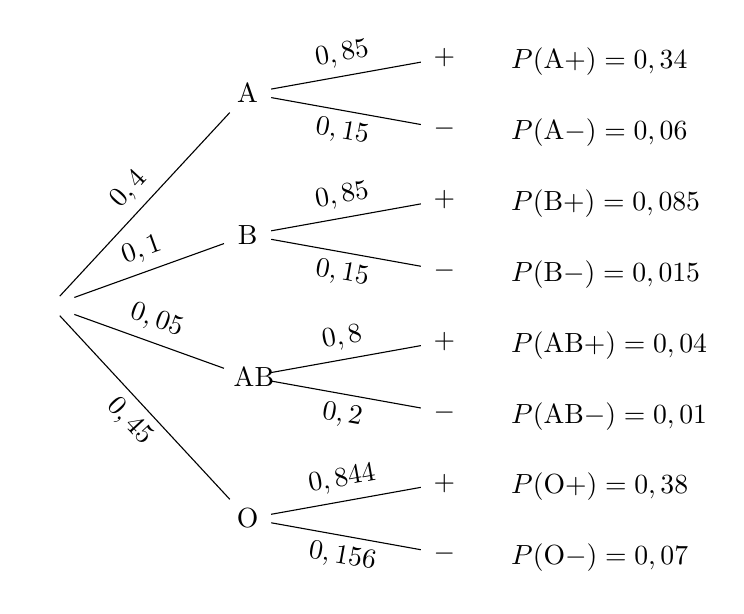
\begin{tikzpicture}[grow=right, sloped]
%wortel
\node[bag] {}
%begin level1-O
    child {
        node[bag] {O}        
%begin level2-O-
        child {
                node[bag] {$-$}
                node[xshift=0.6cm,yshift=-0.05cm, label=right: {$P($O$-)=0,07$}] {}
                edge from parent
                node[below=0.0cm] {$0,156$}
                }
%end level2-O-
%begin level2-O+
        child {
                node[bag] {$+$}
                node[xshift=0.6cm,yshift=-0.05cm, label=right: {$P($O$+)=0,38$}] {}
                edge from parent
                node[above=0.0cm] {$0,844$}
                }
%end level2-O+
        edge from parent
        node[below=0.0cm] {$0,45$}
    }
%end level1-O
%begin level1-AB
    child {
        node[bag] {AB}        
%begin level2-AB-
        child {
                node[bag] {$-$}
                node[xshift=0.6cm,yshift=-0.05cm, label=right: {$P($AB$-)=0,01$}] {}
                edge from parent
                node[below=0.0cm] {$0,2$}
                }
%end level2-AB-
%begin level2-AB+
        child {
                node[bag] {$+$}
                node[xshift=0.6cm,yshift=-0.05cm, label=right: {$P($AB$+)=0,04$}] {}
                edge from parent
                node[above=0.0cm] {$0,8$}
                }
%end level2-AB+
        edge from parent
        node[above=0.0cm] {$0,05$}
    }
%end level1-AB
%begin level1-B
    child {
        node[bag] {B}        
%begin level2-B-
        child {
                node[bag] {$-$}
                node[xshift=0.6cm,yshift=-0.05cm, label=right: {$P($B$-)=0,015$}] {}
                edge from parent
                node[below=0.0cm] {$0,15$}
                }
%end level2-B-
%begin level2-B+
        child {
                node[bag] {$+$}
                node[xshift=0.6cm,yshift=-0.05cm, label=right: {$P($B$+)=0,085$}] {}
                edge from parent
                node[above=0.0cm] {$0,85$}
                }
%end level2-B+
        edge from parent
        node[above=0.0cm] {$0,1$}
    }
%end level1-B
%begin level1-A
    child {
        node[bag] {A}        
%begin level2-A-
        child {
                node[bag] {$-$}
                node[xshift=0.6cm,yshift=-0.05cm, label=right: {$P($A$-)=0,06$}] {}
                edge from parent
                node[below=0.0cm] {$0,15$}
                }
%end level2-A-
%begin level2-A+
        child {
                node[bag] {$+$}
                node[xshift=0.6cm,yshift=-0.05cm, label=right: {$P($A$+)=0,34$}] {}
                edge from parent
                node[above=0.0cm] {$0,85$}
                }
%end level2-A+
        edge from parent
        node[above=0.0cm] {$0,4$}
    };
%end level1-A
%end wortel
\end{tikzpicture}
\caption{Kansboom bloedgroepen en rhesusfactor}
\label{fig:bloed_versie01}
\end{afbeeldingenv}
%einde figuur




%begin figuur
% Set the overall layout of the tree
\tikzstyle{level 1}=[level distance=1.0cm, sibling distance=3.2cm]
\tikzstyle{level 2}=[level distance=3cm, sibling distance=0.8cm]

% Define styles for bags and leafs
\tikzstyle{bag} = [text width=2em, text centered]

\begin{afbeeldingenv}
\hspace{0.2cm}rhesusfactor \hspace{0.5cm}bloedgroep \hspace{0.4cm}kans
\\
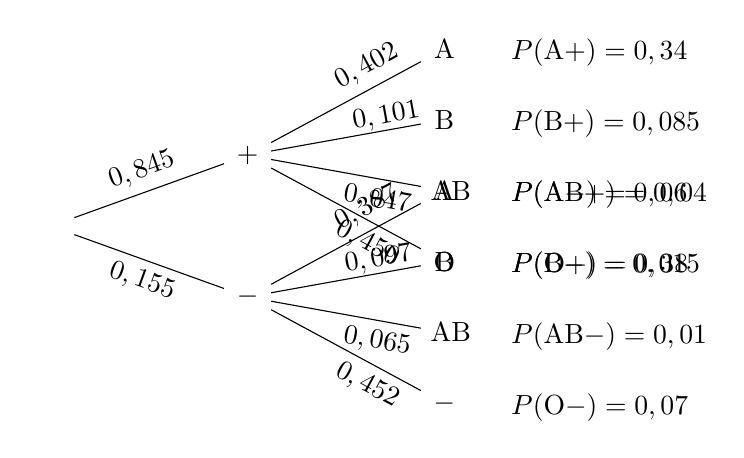
\begin{tikzpicture}[grow=right, sloped]
%wortel
\node[bag] {}
%begin level1-min
    child {
        node[bag] {$-$}        
%begin level2-min-O
        child {
                node[bag] {$-$}
                node[xshift=0.6cm,yshift=-0.05cm, label=right: {$P($O$-)=0,07$}] {}
                edge from parent
                node[below=0.0cm] {\hspace{0.9cm}$0,452$}
                }
%end level2-min-O
%begin level2-min-AB
        child {
                node[bag] {AB}
                node[xshift=0.6cm,yshift=-0.05cm, label=right: {$P($AB$-)=0,01$}] {}
                edge from parent
                node[below=0.0cm] {\hspace{0.9cm}$0,065$}
                }
%end level2-min-AB
%begin level2-min-B
        child {
                node[bag] {B}
                node[xshift=0.6cm,yshift=-0.05cm, label=right: {$P($B$-)=0,015$}] {}
                edge from parent
                node[above=-0.1cm] {\hspace{0.9cm}$0,097$}
                }
%end level2-min-B
%begin level2-min-A
        child {
                node[bag] {A}
                node[xshift=0.6cm,yshift=-0.05cm, label=right: {$P($A$-)=0,06$}] {}
                edge from parent
                node[above=0.0cm] {\hspace{0.9cm}$0,387$}
                }
%end level2-min-A
        edge from parent
        node[below=0.0cm] {$0,155$}
    }
%end level1-min
%begin level1-plus
    child {
        node[bag] {+}        
%begin level2-plus-O
        child {
                node[bag] {O}
                node[xshift=0.6cm,yshift=-0.05cm, label=right: {$P($O$+)=0,38$}] {}
                edge from parent
                node[below=0.0cm] {\hspace{0.9cm}$0,450$}
                }
%end level2-plus-O
%begin level2-plus-AB
        child {
                node[bag] {AB}
                node[xshift=0.6cm,yshift=-0.05cm, label=right: {$P($AB$+)=0,04$}] {}
                edge from parent
                node[below=0.0cm] {\hspace{0.9cm}$0,047$}
                }
%end level2-plus-AB
%begin level2-plus-B
        child {
                node[bag] {B}
                node[xshift=0.6cm,yshift=-0.05cm, label=right: {$P($B$+)=0,085$}] {}
                edge from parent
                node[above=-0.1cm] {\hspace{1.1cm}$0,101$}
                }
%end level2-plus-B
%begin level2-plus-A
        child {
                node[bag] {A}
                node[xshift=0.6cm,yshift=-0.05cm, label=right: {$P($A$+)=0,34$}] {}
                edge from parent
                node[above=0.0cm] {\hspace{0.9cm}$0,402$}
                }
%end level2-plus-A
        edge from parent
        node[above=0.0cm] {$0,845$}
    };
%end level1-plus
%end wortel
\end{tikzpicture}
\caption{Kansboom rhesusfactor en bloedgroepen}
\label{fig:bloed_versie02}
\end{afbeeldingenv}
%einde figuur




\section{Kansrekenen met verzamelingen en stochastische veranderlijken}

De informele aanpak die we in de vorige paragrafen geïllustreerd hebben, laat toe om reeds best veel kansproblemen op te lossen. Voor heel wat studierichtingen kan het hier bij blijven en is alles wat nu volgt in deze loep facultatieve leerinhoud, die je (deels) kunt behandelen als je dat zinvol vindt, maar die niet verplicht is. In een aantal studierichtingen is het echter noodzakelijk om de kansrekening wat meer te formaliseren omdat de specifieke eindtermen dit voorschrijven.

Dit kan in principe op twee verschillende manieren: met verzamelingen en met kansverdelingen van stochastische veranderlijken (dit is de naam die we in deze loep zullen gebruiken; andere gebruikelijke namen zijn: stochastische variabelen, stochasten, toevalsveranderlijken, kansvariabelen…).

Verzamelingen worden in de (specifieke) eindtermen over kansrekenen niet genoemd, en hoeven dus niet per se aan bod te komen. Wel worden Venndiagrammen genoemd in de eindterm over telproblemen in de tweede graad (doorstroomfinaliteit en dubbele finaliteit). Er zit dus een zekere logica in om dit door te trekken naar de kansrekening in de derde graad voor die studierichtingen die verder moeten gaan dan wat tot nu toe in de loep besproken is. Bovendien is het gebruik van verzamelingen in de kansrekening ingeburgerd in ons onderwijs. In \autoref{par:verz} gaan we hier op in.

Kansverdelingen (van een stochastische veranderlijke) worden wél genoemd in de eindtermen. Meer bepaald is er een specifieke eindterm over de binomiale (kans)verdeling, een belangrijke discrete kansverdeling, in het pakket Statistiek (voor bv. de studierichting Humane wetenschappen, eindterm 06.01.02) en in het pakket Gevorderde wiskunde (voor de sterkst wiskundige studierichtingen, eindterm 06.08.35):
\begin{citaat}
De leerlingen berekenen en interpreteren kansen met behulp van de binomiale verdeling.
\end{citaat}

In de (basis)eindtermen doorstroomfinaliteit (eindterm 06.17) en dubbele finaliteit (eindterm 06.10) wordt de normale verdeling genoemd, een continue kansverdeling:
\begin{citaat}
De leerlingen berekenen kansen bij een normaal verdeelde kansvariabele.
\end{citaat}

Kansverdelingen en stochastische veranderlijken in het algemeen worden in de (specifieke) eindtermen niet genoemd en hoeven dus niet per se behandeld te worden. In \autoref{par:stochvar} doen we dat wel en zetten we de stap naar discrete stochastische veranderlijken. Ook deze leerinhouden worden traditioneel vaak behandeld in de sterk wiskundige studierichtingen. Continue stochastische veranderlijken laten we in onze loep buiten beschouwing.

De loep verandert vanaf deze paragraaf wat van toon. We willen nu in de eerste plaats tonen hoe de formulering met verzamelingen en met stochastische veranderlijken samenhangt met kansbomen en kruistabellen. Als je weet hoe deze verschillende ‘gereedschappen’ om aan kansrekening te doen met elkaar samenhangen, kun je in de les een meer coherent verhaal brengen. De aanpak met verzamelingen en stochastische veranderlijken hoeft dan geen nieuwe aanpak te zijn die al het vorige vervangt, maar kansbomen en kruistabellen kunnen blijven functioneren samen met verzamelingen en/of stochastische veranderlijken.

Omdat we de focus willen leggen op de grote, overkoepelende samenhang, kiezen we voor een heel sobere en compacte aanpak, zonder veel didactische verwerking. Ons doel is dat de globale leerlijn zo duidelijk en overzichtelijk mogelijk naar voor komt. We maken hierbij gebruik van enkele terugkerende voorbeelden. We hebben daarbij niet gezocht naar voorbeelden die het maatschappelijke belang van de kansrekening goed in de verf zetten, maar in de eerste plaats naar heel eenvoudige voorbeelden. 

\subsection{Kansrekenen met verzamelingen}
\label{par:verz}
In de vorige paragrafen hebben we kansproblemen opgelost door gebruik te maken van kansbomen en kruistabellen. We zetten nu de stap naar het gebruik van verzamelingen.

\subsection*{De start}

We vertrekken van een eenvoudig discreet kansexperiment waarbij we geen kansboom of kruistabel nodig hebben: we trekken willekeurig een kaart uit een boek kaarten en registeren welke kaart we getrokken hebben. Aan de hand van zo’n voorbeeld kunnen we de klassieke begrippen uit de kansrekening met eindige verzamelingen invoeren:

\begin{itemize}
    \item er zijn 52 \emph{uitkomsten} (als we geen jokers meetellen), namelijk de 52 verschillende kaarten;
    \item de \emph{uitkomstenverzameling} $U$ is de verzameling van deze 52 uitkomsten, dus $U=\{$schoppen aas, schoppen twee, …$\}$;
    \item elke uitkomst heeft een bepaalde \emph{kans}; omdat alle uitkomsten hier even waarschijnlijk zijn en de som van alle kansen gelijk moet zijn aan $1$, heeft elke uitkomst kans $1/52$;
    \item een \emph{gebeurtenis} kunnen we voorstellen als een deelverzameling van de uitkomstenverzameling; bijvoorbeeld: ‘de kaart die we trekken, is een twee’ leidt tot de gebeurtenis $G=\{$schoppen twee, klaveren twee, harten twee, ruiten twee$\}$ (zie \autoref{fig:kaarten_gebeurtenis} hieronder);
    \item de \emph{kans van een gebeurtenis} is de som van de kansen van alle uitkomsten uit deze gebeurtenis; omdat de kansen van alle uitkomsten hier even groot zijn, is de kans $P(G)$ van een gebeurtenis $G$ gelijk aan $\#G/\#U$;
    \item eventueel kunnen we een \emph{kansfunctie} $P$ invoeren, die elke deelverzameling van $U$ afbeeldt op zijn kans, dus $P:\mathcal{D}(U) \rightarrow [0,1]:G \mapsto P(G)$.
\end{itemize}

\begin{afbeeldingenv}
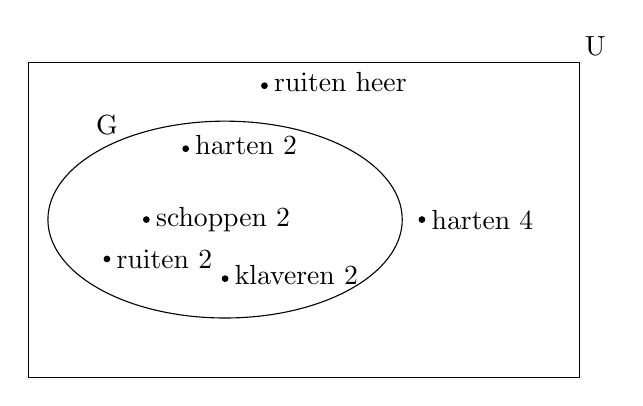
\begin{tikzpicture}
\draw (0,0) rectangle (7,4) ; 
\draw (2.5,2) ellipse (2.25cm and 1.25cm);
\draw[fill] (1.5,2) circle (1pt);
\draw[fill] (1,1.5) circle (1pt);
\draw[fill] (2,2.9) circle (1pt);
\draw[fill] (2.5,1.25) circle (1pt);
\draw[fill] (5,2) circle (1pt);
\draw[fill] (3,3.7) circle (1pt);
\node[xshift=7.2cm,yshift=4.2cm] {U};
\node[xshift=1cm,yshift=3.2cm] {G};
\node[xshift=1.5cm,yshift=2cm, right] {schoppen 2};
\node[xshift=1cm,yshift=1.5cm, right] {ruiten 2};
\node[xshift=2.5cm,yshift=1.3cm, right] {klaveren 2};
\node[xshift=2cm,yshift=2.95cm, right] {harten 2};
\node[xshift=5cm,yshift=2cm, right] {harten 4};
\node[xshift=3cm,yshift=3.75cm, right] {ruiten heer};
\end{tikzpicture}
\caption{Gebeurtenis als deelverzameling van het universum}
\label{fig:kaarten_gebeurtenis}
\end{afbeeldingenv}

De overstap naar gebeurtenissen als verzamelingen is geen heel grote stap, maar houdt op een aantal punten toch wel een subtiele verandering in. Zo zullen we nu bijvoorbeeld symbolen uit de verzamelingenleer gebruiken om ‘samengestelde’ gebeurtenissen te beschrijven. Een voorbeeld: als $S$ de gebeurtenis voorstelt dat de getrokken kaart een schoppen is en $E$ de gebeurtenis dat er op de getrokken kaart een getal staat dat even is, dan noteren we $S \cap E$ voor de gebeurtenis dat de getrokken kaart een schoppen met een even getal is.

In de voorgaande paragrafen hebben we gebeurtenissen in feite beschouwd als uitspraken over de uitkomst van het kansexperiment. De bovenstaande samengestelde gebeurtenis kunnen we dan omschrijven met een bewerking uit de logica: ‘de kaart die we trekken, is een schoppen \underline{en} de kaart die we trekken, bevat een even getal’.

\subsection*{Verzamelingen en kruistabellen}

We gaan verder met het kansexperiment over het trekken van een kaart, maar nu uit een onvolledige set van 10 kaarten. De set bestaat uit S2, SD, K4, K6, K7, KH, H3, H7, H9 en RD (waarbij, bijvoorbeeld, RD de ruiten dame aangeeft). We trekken nog altijd één kaart, en letten enerzijds op de soort en anderzijds of er een getal op staat, dan wel een figuur. We geven de kansen weer in de onderstaande kruistabel (\autoref{tab:kaartvb}).

\begin{tabel}
\begin{tabular}{m{2.2cm} C{1.5cm} C{1.5cm} C{1.5cm}}
	\hlinethick
	\tableheader{} & \tableheader{getal} & \tableheader{figuur} & \tableheader{totaal} \\
	\hlinethick
		schoppen & $0,1$ & $0,1$ & $0,2$ \\
		klaveren & $0,3$ & $0,1$ & $0,4$  \\
		harten  & $0,3$ & $0$ & $0,3$ \\
           ruiten & $0$ & $0,1$ & $0,1$ \\
           totaal & $0,7$ & $0,3$ & $1$ \\
	\hlinethick
	\end{tabular}
	\caption{Kruistabel bij het kansexperiment over het trekken van een kaart uit een onvolledige set van 10 kaarten}\label{tab:kaartvb}
	\end{tabel}

De eigenschappen die in de linkse kolom en in de bovenste rij staan, verwijzen naar gebeurtenissen. We gebruiken bijvoorbeeld de notatie $G$ om de gebeurtenis weer te geven dat de kaart die we trekken een getal bevat: $G=\{$S2, K4, K6, K7, H3, H7, H9$\}$. Analoog gebruiken we de notaties $F$, $S$, $K$, $H$ en $R$. De marginale kansen zijn dan $P(S)=0,2$, $P(K)=0,4$, $P(H)=0,3$ en $P(R)=0,1$ (in de rechterkolom) en $P(G)=0,7$ en $P(F)=0,3$ (onderaan).

Ook de gebeurtenissen die overeenkomen met de cellen in het ‘midden’ van de kruistabel, kunnen we voorstellen met deze verzamelingen. Linksboven vinden we bijvoorbeeld de kans $P(S \cap G)=P(\{$S2$\}$), de kans dat de getrokken kaart een schoppen is en dat ze een getal bevat. In elke cel staat de kans van de doorsnede van twee gebeurtenissen, de gebeurtenis die overeenkomt met de rij waarin de cel zich bevindt, en de gebeurtenis die overeenkomt met de kolom.

We vatten alles samen in onderstaande kruistabel (zie \autoref{tab:kaartvb_verz}):

\begin{tabel}
    \begin{tabular}{m{1.6cm} C{1.8cm} C{1.8cm} C{1.5cm}}
	\hlinethick
	\tableheader{} & \tableheader{$G$} & \tableheader{$F$} & \tableheader{totaal} \\
	\hlinethick
		$S$ & $P(S \cap G)$ & $P(S \cap F)$ & $P(S)$ \\
		$K$ & $P(K \cap G)$ & $P(K \cap F)$ & $P(K)$  \\
		$H$  & $P(H \cap G)$ & $P(H \cap F)$ & $P(H)$ \\
        $R$ & $P(R \cap G)$ & $P(R \cap F)$ & $P(R)$ \\
        totaal & $P(G)$ & $P(F)$ & $1$ \\
	\hlinethick
	\end{tabular}
    \caption{Kruistabel met een overzicht van de kansen in termen van verzamelingen bij het kansexperiment over het trekken van een kaart uit een onvolledige set van 10 kaarten}\label{tab:kaartvb_verz}
\end{tabel}

Essentieel bij zo’n kruistabel is

\begin{itemize}
    \item dat de gebeurtenissen in de linkerkolom elkaar uitsluiten, of met verzamelingenterminologie: dat de gebeurtenissen twee aan twee disjunct zijn (d.w.z. dat hun doorsnede twee aan twee leeg is);
    \item dat ze samen alle uitkomsten bevatten ($S \cup K \cup H \cup R=U$).
\end{itemize}

In de wiskunde benoemt men dit als volgt: de gebeurtenissen $S$, $K$, $H$ en $R$ vormen een \emph{partitie} van de uitkomstenverzameling.

Dit geldt natuurlijk ook voor de categorieën in de bovenste rij: ook $G$ en $F$ vormen een partitie van de uitkomstenverzameling. Omdat er maar twee categorieën zijn, betekent dit dat $G$ en $F$ elkaars complement zijn, dus bijvoorbeeld $F=G^C$. Met andere woorden: $F$ bestaat uit de uitkomsten die geen getal bevatten. Of nog: de eigenschap ‘de kaart die we trekken, bevat een getal’ is wel aanwezig (gebeurtenis $G$) of niet aanwezig (gebeurtenis $F$).

Een marginale kans is natuurlijk de som van de kansen uit dezelfde rij of kolom van het middengedeelte van de tabel. Bijvoorbeeld: 
$$P(G)=P(S \cap G)+P(K \cap G)+P(H \cap G)+P(R \cap G).$$

Dit is in feite niets anders dan de wet van de totale kans.

\subsection*{Kruistabellen en Venndiagrammen}

We hebben in deze paragraaf al een paar keer een Venndiagram gebruikt als illustratie. We bekijken de situatie van een 2-bij-2-kruistabel nu wat meer in detail. We werken met een vereenvoudigde versie van het bovenstaande kaartexperiment (zie \autoref{tab:kaartvb_2bij2}, waarbij we nu enkel letten op de kleur van de kaart (zwart of rood, twee rijen) en of er een getal of een figuur op staat (twee kolommen)).

\begin{tabel}
    \begin{tabular}{m{2.2cm} C{1.5cm} C{1.5cm} C{1.5cm}}
	\hlinethick
	\tableheader{} & \tableheader{getal} & \tableheader{figuur} & \tableheader{totaal} \\
	\hlinethick
		zwart & $0,4$ & $0,2$ & $0,6$ \\
		rood & $0,3$ & $0,1$ & $0,4$  \\
        totaal & $0,7$ & $0,3$ & $1$ \\
	\hlinethick
	\end{tabular}
    \caption{Kruistabel bij het vereenvoudigde kansexperiment over het trekken van een kaart uit een onvolledige set van 10 kaarten}
    \label{tab:kaartvb_2bij2}
\end{tabel}

De informatie die in deze 2-bij-2-kruistabel weergegeven is, is in \autoref{fig:kaartvb_2bij2}
weergegeven met een Venndiagram. 

\begin{afbeeldingenv}
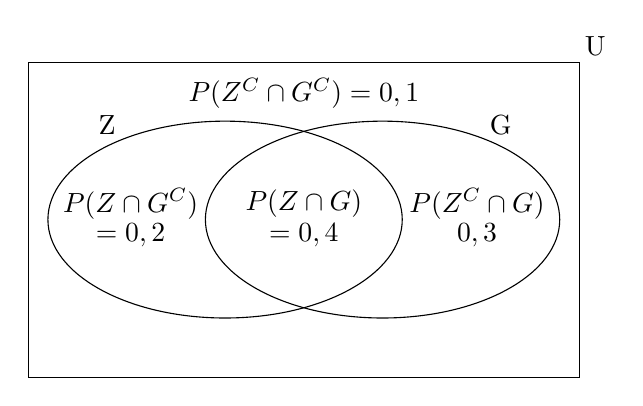
\begin{tikzpicture}
\draw (0,0) rectangle (7,4) ; 
\draw (2.5,2) ellipse (2.25cm and 1.25cm);
\draw (4.5,2) ellipse (2.25cm and 1.25cm);
\node[xshift=7.2cm,yshift=4.2cm] {U};
\node[xshift=1cm,yshift=3.2cm] {Z};
\node[xshift=6cm,yshift=3.2cm] {G};
\node[xshift=3.5cm,yshift=2.2cm] {$P(Z\cap G)$};
\node[xshift=3.5cm,yshift=1.8cm] {$=0,4$};
\node[xshift=1.3cm,yshift=2.2cm] {$P(Z\cap G^C)$};
\node[xshift=1.3cm,yshift=1.8cm] {$=0,2$};
\node[xshift=5.7cm,yshift=2.2cm] {$P(Z^C\cap G)$};
\node[xshift=5.7cm,yshift=1.8cm] {$0,3$};\node[xshift=3.5cm,yshift=3.6cm] {$P(Z^C \cap G^C)=0,1$};
\end{tikzpicture}
\caption{Venndiagram bij het vereenvoudigde kansexperiment over het trekken van een kaart uit een onvolledige set van 10 kaarten}
\label{fig:kaartvb_2bij2}
\end{afbeeldingenv}

We zien in de figuur vier gebieden, die overeenkomen met de middelste vier cellen uit de kruistabel. We hebben slechts twee gebeurtenissen expliciet voorgesteld. Een kruistabel heeft twee ‘dimensies’. Uit elk van beide dimensies kiezen we een van beide gebeurtenissen. Meer bepaald, uit de eerste kolom hebben we $Z$ voorgesteld, de verzameling die overeenkomt met de gebeurtenis ‘de kaart die we trekken, is zwart’. De andere gebeurtenis, namelijk ‘de kaart die we trekken, is rood’, zien we in het Venndiagram niet expliciet voorkomen, maar ze is het complement van $Z$. Ook uit de bovenste rij van de kruistabel stellen we een van beide gebeurtenissen expliciet voor, namelijk $G$. De andere gebeurtenis is het complement van $G$. We hebben in elk gebied de overeenkomstige kans aangeduid.

In situaties met meer dan twee categorieën is een voorstelling met een Venndiagram in principe nog wel mogelijk maar is ze weinig verhelderend. Zie bijvoorbeeld \autoref{fig:kaartvb} hieronder waarin we het Venndiagram bij het oorspronkelijke kaartexperiment (vier soorten i.p.v. twee kleuren) voorstellen.

\begin{afbeeldingenv}
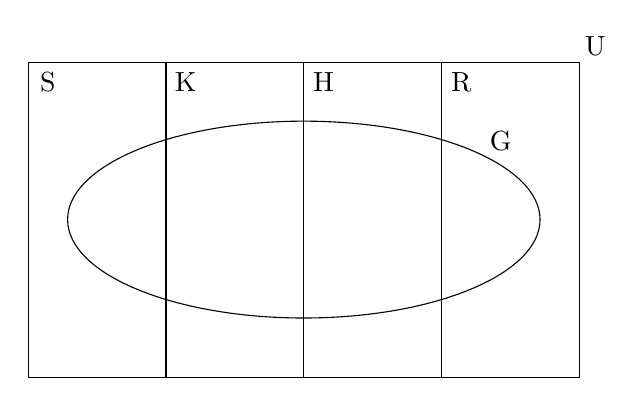
\begin{tikzpicture}
\draw (0,0) rectangle (7,4) ; 
\draw (3.5,2) ellipse (3cm and 1.25cm);
\draw (1.75,0) -- (1.75,4);
\draw (3.5,0) -- (3.5,4);
\draw (5.25,0) -- (5.25,4);
\node[xshift=7.2cm,yshift=4.2cm] {U};
\node[xshift=6cm,yshift=3cm] {G};
\node[xshift=0.25cm,yshift=3.75cm] {S};
\node[xshift=2.0cm,yshift=3.75cm] {K};
\node[xshift=3.75cm,yshift=3.75cm] {H};
\node[xshift=5.5cm,yshift=3.75cm] {R};
\end{tikzpicture}
\caption{Venndiagram bij het oorspronkelijke kansexperiment over het trekken van een kaart uit een onvolledige set van 10 kaarten}
\label{fig:kaartvb}
\end{afbeeldingenv}

\subsection*{Verzamelingen en kansbomen}
Nu we gezien hebben dat we alle kansen in een kruistabel kunnen relateren aan eenvoudige gebeurtenissen, onderzoeken we of dit ook het geval is bij kansbomen. Het zal blijken dat dit inderdaad ook kan, maar voorlopig nog niet volledig (en dat zal de aanleiding zijn voor de volgende paragraaf, over voorwaardelijke kansen).

We gaan verder met het kansexperiment dat we bij de kruistabel gebruikten en stellen eerst een kansboom op (zie \autoref{fig:kansboom_kaartvb}).


%begin van de figuur
% Set the overall layout of the tree
\tikzstyle{level 1}=[level distance=2.5cm, sibling distance=1.5cm]
\tikzstyle{level 2}=[level distance=2.5cm, sibling distance=0.75cm]

% Define styles for bags and leafs
\tikzstyle{bag} = [text width=1em, text centered]
\tikzstyle{end} = [circle, minimum width=0pt,fill, inner sep=0pt]

\begin{afbeeldingenv}
\hspace{2.8cm}soort \hspace{1.0cm}getal of figuur?\\
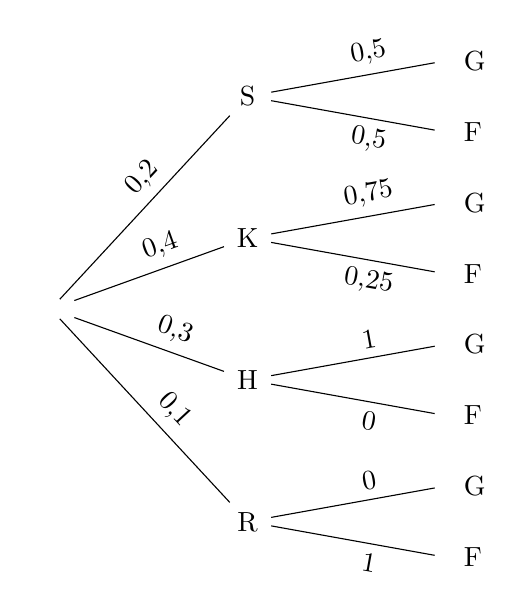
\begin{tikzpicture}[grow=right, sloped]
\node[bag] {}
    child {
        node[bag] {R}        
           child {
                node[end, label=right: {F}] {}
                edge from parent
                node[below=0cm] {\hspace{0.5cm}1}
                            }
           child {
                node[end, label=right: {G}] {}
                edge from parent
                node[above=0cm] {\hspace{0.5cm}0}
                            }
           edge from parent 
           node[above=0cm] {\hspace{0.5cm}0,1}
    }
    child {
        node[bag] {H}        
           child {
                node[end, label=right: {F}] {}
                edge from parent
                node[below=0cm] {\hspace{0.5cm}0}
                            }
           child {
                node[end, label=right: {G}] {}
           edge from parent
           node[above=0cm] {\hspace{0.5cm}1}
                            }
           edge from parent 
           node[above=0cm] {\hspace{0.5cm}0,3}
    }
    child {
        node[bag] {K}        
           child {
                node[end, label=right: {F}] {}
                edge from parent
                node[below=0cm] {\hspace{0.5cm}0,25}
                            }
            child {
                node[end, label=right: {G}] {}
                edge from parent
                node[above=0cm] {\hspace{0.5cm}0,75}
                            }
           edge from parent 
           node[above=0cm] {\hspace{0.5cm}0,4}
    }
    child {
        node[bag] {S}        
           child {
                node[end, label=right: {F}] {}
                edge from parent
                node[below=0cm] {\hspace{0.5cm}0,5}
                            }
            child {
                node[end, label=right: {G}] {}
                edge from parent
                node[above=0cm] {\hspace{0.5cm}0,5}
                            }
           edge from parent 
           node[above=0cm] {\hspace{0.5cm}0,2}
    };
\end{tikzpicture}
\caption{Kansboom bij het kansexperiment over het trekken van een kaart uit een onvolledige set van 10 kaarten}
\label{fig:kansboom_kaartvb}
\end{afbeeldingenv}
%einde van de figuur

De gebeurtenissen $S$, $K$, $H$ en $R$ houden verband met de eerste vertakking in de kansboom en op de takken zien we in \autoref{fig:kansboom_kaartvb_verz}
hieronder dan ook de kansen $P(S)$, $P(K)$, $P(H)$ en $P(R)$. De acht kansen bij de bladeren helemaal rechts zijn de kansen van doorsneden.

%begin van de figuur
% Set the overall layout of the tree
\tikzstyle{level 1}=[level distance=2.5cm, sibling distance=1.5cm]
\tikzstyle{level 2}=[level distance=2.5cm, sibling distance=0.75cm]

% Define styles for bags and leafs
\tikzstyle{bag} = [text width=1em, text centered]

\begin{afbeeldingenv}
\hspace{2cm}soort \hspace{1cm}getal of figuur?\\
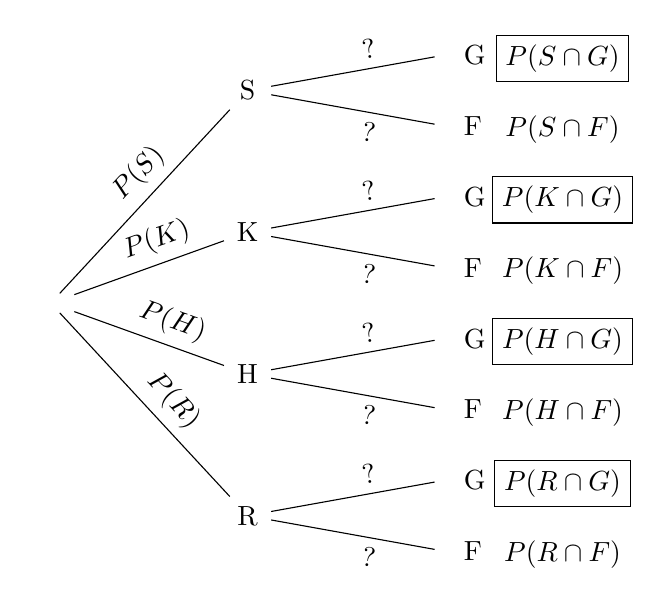
\begin{tikzpicture}[grow=right, sloped]
\node[bag] {}
    child {
        node[bag] {R}        
           child {
                node[end, label=right: {F}] {}
                node[xshift=1.5cm,yshift=-0.04cm] {$P(R \cap F)$}
                edge from parent
                node[below=0cm] {\hspace{0.5cm}?} 
                            }
           child {
                node[end, label=right: {G}] {}
                node[rectangle,draw,xshift=1.5cm,yshift=-0.04cm] {$P(R \cap G)$}
                edge from parent
                node[above=0cm] {\hspace{0.5cm}?}
                            }
           edge from parent 
           node[above=0cm] {\hspace{0.3cm} $P(R)$}
    }
    child {
        node[bag] {H}        
           child {
                node[end, label=right: {F}] {}
                node[xshift=1.5cm,yshift=-0.04cm] {$P(H \cap F)$}
                edge from parent
                node[below=0cm] {\hspace{0.5cm}?}
                            }
           child {
                node[end, label=right: {G}] {}
                node[rectangle,draw,xshift=1.5cm,yshift=-0.04cm] {$P(H \cap G)$}
                edge from parent
                node[above=0cm] {\hspace{0.5cm}?}
                            }
           edge from parent 
           node[above=0cm] {\hspace{0.3cm} $P(H)$}
    }
    child {
        node[bag] {K}        
           child {
                node[end, label=right: {F}] {}
                node[xshift=1.5cm,yshift=-0.04cm] {$P(K \cap F)$}
                edge from parent
                node[below=0cm] {\hspace{0.5cm}?}
                            }
            child {
                node[end, label=right: {G}] {}
                node[rectangle,draw,xshift=1.5cm,yshift=-0.04cm] {$P(K \cap G)$}
                edge from parent
                node[above=0cm] {\hspace{0.5cm}?}
                            }
           edge from parent 
           node[above=0cm] {\hspace{0.3cm} $P(K)$}
    }
    child {
        node[bag] {S}        
           child {
                node[end, label=right: {F}] {}
                node[xshift=1.5cm,yshift=-0.04cm] {$P(S \cap F)$}
                edge from parent
                node[below=0cm] {\hspace{0.5cm}?}
                            }
            child {
                node[end, label=right: {G}] {}
                node[rectangle,draw,xshift=1.5cm,yshift=-0.04cm] {$P(S \cap G)$}
                edge from parent
                node[above=0cm] {\hspace{0.5cm}?}
                            }
           edge from parent 
           node[above=0cm] {\hspace{0.3cm} $P(S)$}
    };
\end{tikzpicture}
\caption{Kansboom bij het kansexperiment over het trekken van een kaart uit een onvolledige set van 10 kaarten met kansen uitgedrukt als kansen van gebeurtenissen}
\label{fig:kansboom_kaartvb_verz}
\end{afbeeldingenv}
%einde van de figuur

De gebeurtenissen $G$ en $F$ en hun kansen vinden we niet rechtstreeks in de kansboom terug (wél in de kruistabel, zagen we hierboven). Om deze kansen te kennen, moeten we vier van de bladeren samen nemen (zie de kadertjes in bovenstaande figuur), bijvoorbeeld
$$P(G)=P(S \cap G)+P(K \cap G)+P(H \cap G)+P(R \cap G).$$
We stellen dus vast dat bij een kansboom de twee eigenschappen waar op gelet wordt (soort en getal/figuur) een verschillende rol spelen. Bij een kruistabel daarentegen spelen ze een evenwaardige rol.

De kansen bij de takken van de tweede generatie kunnen we voorlopig nog niet noteren met behulp van de gebeurtenissen die we onderscheiden hebben. Dat zullen we in de volgende paragraaf oplossen.

Bij de kruistabel zagen we dat de gebeurtenissen $S$, $K$, $H$ en $R$ twee aan twee disjunct zijn en dat hun unie de hele uitkomstenverzameling is, en we hebben toen ook de naam genoemd die hiervoor in de wiskunde gebruikt wordt: $S$, $K$, $H$ en $R$ vormen een partitie van de uitkomstenverzameling. Ook bij de kansboom is deze eigenschap belangrijk: elke uitkomst hoort bij juist één van de vier takken die in de wortel vertrekken. Deze eigenschap ligt aan de basis van de gekende eigenschap dat de som van de kansen van de takken uit eenzelfde knooppunt $1$ is. Ook voor de takken van de tweede generatie geldt deze eigenschap, maar daar is het wat ingewikkelder om de achterliggende eigenschap met verzamelingen te zien. We komen hier op terug in de volgende paragraaf.

\subsection*{Een veralgemeende somregel}
We hebben bij de kansbomen en bij de kruistabellen geregeld kansen opgeteld. In het voorbeeld met de kansboom deden we het daarnet nog om de kans $P(G)$ op een kaart met een getal te bepalen. Ook bij de kruistabel tellen we soms kansen bij elkaar op. Bijvoorbeeld: de kans op een zwarte kaart met een getal ($0,4$) is de som van de kansen in de overeenkomstige twee cellen ($0,1+0,3$). Dat we in deze twee situaties de kansen zonder meer mogen optellen is een gevolg van het feit dat we te maken hebben met disjuncte gebeurtenissen.

De \emph{veralgemeende} somregel leert ons hoe we de kans berekenen van de unie van twee gebeurtenissen wanneer deze gebeurtenissen niet per se disjunct zijn: 
$$P(G_1 \cup G_2 )=P(G_1 )+P(G_2 )-P(G_1 \cap G_2).$$ 
Deze veralgemeende somregel komt goed tot zijn recht als je gebruik maakt van de voorstelling met Venndiagrammen (zie \autoref{fig:Venn_veralgemeende_somregel} hieronder).

\begin{afbeeldingenv}
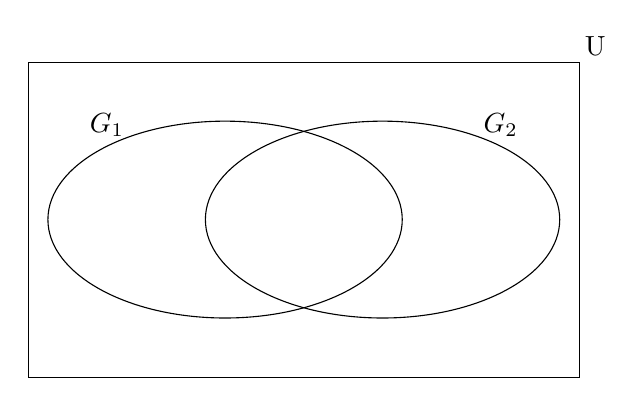
\begin{tikzpicture}
\draw (0,0) rectangle (7,4) ; 
\draw (2.5,2) ellipse (2.25cm and 1.25cm);
\draw (4.5,2) ellipse (2.25cm and 1.25cm);
\node[xshift=7.2cm,yshift=4.2cm] {U};
\node[xshift=1cm,yshift=3.2cm] {$G_1$};
\node[xshift=6cm,yshift=3.2cm] {$G_2$};
\end{tikzpicture}
\caption{Venndiagram bij de veralgemeende somregel}
\label{fig:Venn_veralgemeende_somregel}
\end{afbeeldingenv}

Je moet de kans van de doorsnede aftrekken omdat deze zowel meegerekend is in $P(G_1)$ als in $P(G_2)$. Deze veralgemeende somregel is natuurlijk een echo van de veralgemeende somregel die leerlingen in de tweede graad bij telproblemen ontmoet hebben. 

Je past deze veralgemeende somregel bijvoorbeeld toe als je de kans wil berekenen dat de getrokken kaart een schoppen is of een kaart met een getal op. Als je de twee marginale kansen $P(S)$ en $P(G)$ optelt, heb je de schoppen met een getal dubbel meegerekend en moet je die dus één keer aftrekken:
\begin{equation*}
\begin{split}
P(S \cup G) &=P(S)+P(G)-P(S \cap G)\\
 & =0,2+0,7-0,1=0,8.
\end{split}
\end{equation*}

\subsection*{Axioma’s voor de kansrekening}
Aansluitend bij het behandelen van de kansrekening met verzamelingen, zou je ook de stap kunnen zetten naar een stel axioma’s voor de eindige kansrekening.

Een \emph{eindige kansruimte} bestaat uit een eindige verzameling $U$ en een kansfunctie $P$ die elke deelverzameling $G$ van $U$ afbeeldt op een getal $P(G)$ in het interval $[0,1]$, met als eigenschappen:
\begin{itemize}
    \item $P(\emptyset)=0$;
    \item $P(U)=1$;
    \item $P(G_1 \cup G_2)=P(G_1)+P(G_2)$ als $G_1$ en $G_2$ disjuncte gebeurtenissen zijn.
\end{itemize}
Het biedt de gelegenheid om leerlingen te laten kennismaken met een eenvoudig axiomasysteem, wat in andere deelgebieden van de wiskunde in het secundair onderwijs praktisch niet mogelijk is. Zo’n axiomatische beschrijving van de kansrekening maakt abstractie van de betekenis van de kans van een gebeurtenis. In de definitie van een kansruimte wordt dus geen poging gedaan om vast te leggen wat een kans precies is. Het is een \emph{ongedefinieerd basisbegrip}. 

Wel legt de definitie van een kansruimte een aantal basiseigenschappen van deze ongedefinieerde basisbegrippen vast. Vergelijk dit met een axiomatische beschrijving van de ruimtemeetkunde. Daar zijn punten, rechten en vlakken ongedefinieerde basisbegrippen, waarvan enkel een aantal basiseigenschappen gegeven worden.

Dat neemt natuurlijk niet weg dat het erg nuttig is als je ‘weet’ wat een punt, rechte of vlak is als je de meetkunde wil gebruiken om iets te leren over de fysische ruimte om ons heen. Net zo is het natuurlijk heel nuttig dat onze leerlingen wel degelijk begrijpen hoe je een kans kunt toekennen aan een gebeurtenis: via de regel van Laplace (‘weetkansen’) of via de frequentiedefinitie (en dus door een kansexperiment heel vaak te herhalen, ‘zweetkansen’). We pleiten er zeker niet voor om dit weg te laten. Integendeel, didactisch gezien is het juist goed om voldoende stil te staan bij het kansbegrip.

Geen van bovenstaande twee klassiek gebruikte omschrijvingen van het begrip kans leent zich echter om een wiskundige definitie van een kans te geven. De regel van Laplace is circulair: hij geldt enkel wanneer uitkomsten even waarschijnlijk zijn, en vertrekt dus van kansen die al gekend zijn. Bij de frequentiedefinitie zou je het kansexperiment oneindig vaak moeten herhalen. 

Meer algemeen: er is geen enkele manier om met wiskundige precisie te omschrijven wat het begrip ‘kans’ inhoudt, net zoals dat het geval is bij het begrip ‘punt’ in de meetkunde. De oplossing bestaat er in om dit begrip niet te definiëren. Het is, zoals hierboven al aangegeven, een ongedefinieerd basisbegrip in een axiomasysteem.

We beperken ons bij deze axiomatische beschrijving tot eindige kansruimten. Uitbreiding tot aftelbaar oneindige kansruimten is nog haalbaar, maar het axiomasysteem (van Kolmogorov uit 1933) voor algemenere oneindige kansruimten is een stuk ingewikkelder. Er kan dan niet langer een kans toegekend worden aan alle deelverzamelingen van de uitkomstenverzameling. De kansfunctie beperkt zich in dat geval tot een zogenaamde sigma-algebra van deelverzamelingen. Dit algemene axiomasysteem is enkel spek voor de bek van universitaire opleidingen wiskunde en statistiek.

\subsection{Kansrekenen met stochastische veranderlijken}
\label{par:stochvar}
We grijpen terug naar het voorbeeld van de volleybalmatch met de ploeg van Samir (zie \autoref{fig:volleybal_3sets} uit \autoref{par:boom}): we spelen drie sets, waarbij de ploeg van Samir elke set 60\% kans heeft om te winnen en waarbij we ervan uitgaan dat het resultaat van een set niet beïnvloed wordt door het resultaat van eerdere sets.



Nu letten we op het aantal keer dat de ploeg van Samir wint. Aan de hand van dit voorbeeld voeren we de klassieke begrippen rond stochastische veranderlijken in:
\begin{itemize}
    \item de mogelijke uitkomsten van het kansexperiment beschrijven we nu aan de hand van een \emph{stochastische veranderlijke}: $X =$ aantal keer dat de ploeg van Samir wint; $X$ kan de waarden $0$, $1$, $2$ of $3$ aannemen (zie de waarden van $X$ bij de bladeren in \autoref{fig:Samir_sv});
    \item de \emph{kansverdeling} van een stochastische veranderlijke geeft voor elke uitkomst de kans van deze uitkomst; de kansverdeling kan voorgesteld worden via een tabel (zie \autoref{tab:Samir_sv}), een grafiek of een formule; in dit geval kunnen we de kansen gemakkelijk afleiden uit het boomdiagram; de som van alle kansen moet gelijk zijn aan 1;

\begin{tabel}
    \begin{tabular}{C{2.8cm} C{3.5cm}}
	\hlinethick
	\tableheader{aantal keer dat de ploeg van Samir wint} & \tableheader{kans} \\
	\hlinethick
		$0$ & $0,4^3=0,064$ \\
		$1$ & $3 \cdot 0,6 \cdot 0,4^2=0,288$ \\
        $2$ & $3 \cdot 0,6^2 \cdot 0,4=0,432$ \\	
        $3$ & $0,6^3=0,216$ \\
        \hlinethick
	\end{tabular}
    \caption{Kansverdeling van de stochastische veranderlijke die telt hoeveel keer de ploeg van Samir wint}
    \label{tab:Samir_sv}
\end{tabel}

    \item \emph{gebeurtenissen} worden nu beschreven in termen van de stochastische veranderlijke, zoals bijvoorbeeld in $P(X=1)=0,288$ en $P(X \leq 2)=0,784$;
    \item verwachtingswaarde en standaardafwijking zijn typische begrippen die nu ingevoerd kunnen worden, maar daar gaan we in deze loep niet op in.
\end{itemize}

\vspace{1 cm}
%begin figuur
% Set the overall layout of the tree
\tikzstyle{level 1}=[level distance=0.7cm, sibling distance=4.4cm]
\tikzstyle{level 2}=[level distance=0.7cm, sibling distance=2.2cm]
\tikzstyle{level 3}=[level distance=0.7cm, sibling distance=1.1cm]


% Define styles for bags and leafs
\tikzstyle{bag} = [text width=1em, text centered]

\begin{afbeeldingenv}
\small
\hspace{-.30cm}set 1 \hspace{0.1cm}set 2 \hspace{0.0cm}set 3 \hspace{0.0cm} spelverloop \hspace{0.2cm} $X$  \hspace{0.1cm}   kans
\normalsize
\\
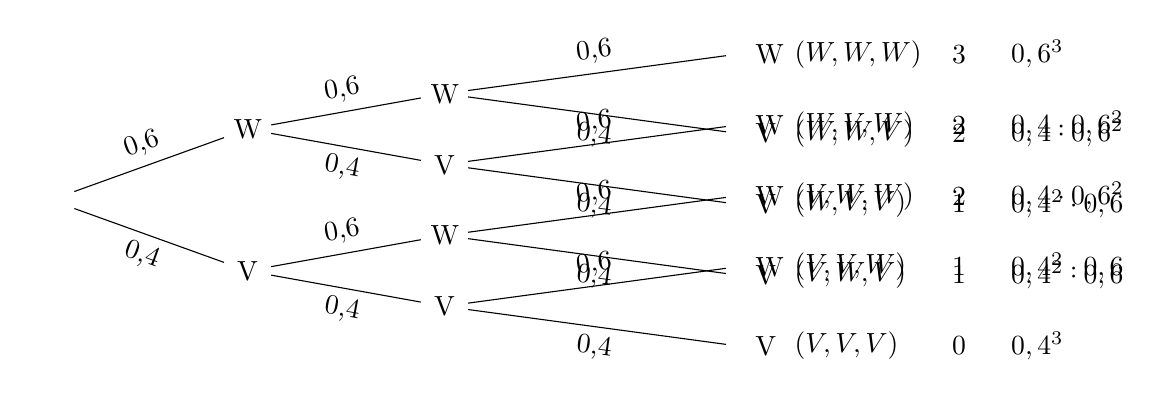
\begin{tikzpicture}[grow=right, sloped]
\node[bag] {}
    child {
        node[bag] {V}        
           child {
                node[bag] {V}
                child {
                    node[end, label=right: {V}] {}
                    node[xshift=0.5cm,yshift=-0cm, label=right: {$(V,V,V)$}] {}
                    node[xshift=2.5cm,yshift=-0cm, label=right: {$0$}] {}
                    node[xshift=3.25cm,yshift=-0cm, label=right: {$0,4^3$}] {}
                    edge from parent
                    node[below=0cm] {\hspace{0.0cm}0,4}
                }
                child {
                    node[end, label=right: {W}] {}
                    node[xshift=0.5cm,yshift=-0cm, label=right: {$(V,V,W)$}] {}
                    node[xshift=2.5cm,yshift=-0cm, label=right: {$1$}] {}
                    node[xshift=3.25cm,yshift=-0cm, label=right: {$0,4^2\cdot0,6$}] {}
                    edge from parent
                    node[above=0cm] {\hspace{0.0cm}0,6}
                }
                edge from parent
                node[below=0cm] {\hspace{0.0cm}0,4} 
           }
           child {
                node[bag] {W}
                child {
                    node[end, label=right: {V}] {}
                    node[xshift=0.5cm,yshift=-0cm, label=right: {$(V,W,V)$}] {}
                    node[xshift=2.5cm,yshift=-0cm, label=right: {$1$}] {}
                    node[xshift=3.25cm,yshift=-0cm, label=right: {$0,4^2\cdot0,6$}] {}
                    edge from parent
                    node[below=0cm] {\hspace{0.0cm}0,4}
                }    
                child {
                    node[end, label=right: {W}] {}
                    node[xshift=0.5cm,yshift=-0cm, label=right: {$(V,W,W)$}] {}
                    node[xshift=2.5cm,yshift=-0cm, label=right: {$2$}] {}
                    node[xshift=3.25cm,yshift=-0cm, label=right: {$0,4\cdot0,6^2$}] {}
                    edge from parent
                    node[above=0cm] {\hspace{0.0cm}0,6}
                }
                edge from parent
                node[above=0cm] {\hspace{0.0cm}0,6} 
            }
        edge from parent
        node[below=0cm] {\hspace{0.0cm}0,4} 
    }
    child {
        node[bag] {W}        
           child {
                node[bag] {V}
                child {
                    node[end, label=right: {V}] {}
                    node[xshift=0.5cm,yshift=-0cm, label=right: {$(W,V,V)$}] {}
                    node[xshift=2.5cm,yshift=-0cm, label=right: {$1$}] {}
                    node[xshift=3.25cm,yshift=-0cm, label=right: {$0,4^2\cdot0,6$}] {}
                    edge from parent
                    node[below=0cm] {\hspace{0.0cm}0,4}
                }
                child {
                    node[end, label=right: {W}] {}
                    node[xshift=0.5cm,yshift=-0cm, label=right: {$(W,V,W)$}] {}
                    node[xshift=2.5cm,yshift=-0cm, label=right: {$2$}] {}
                    node[xshift=3.25cm,yshift=-0cm, label=right: {$0,4\cdot0,6^2$}] {}
                    edge from parent
                    node[above=0cm] {\hspace{0.0cm}0,6}
                }
                edge from parent
                node[below=0cm] {\hspace{0.0cm}0,4} 
           }
           child {
                node[bag] {W}
                child {
                    node[end, label=right: {V}] {}
                    node[xshift=0.5cm,yshift=-0cm, label=right: {$(W,W,V)$}] {}
                    node[xshift=2.5cm,yshift=-0cm, label=right: {$2$}] {}
                    node[xshift=3.25cm,yshift=-0cm, label=right: {$0,4\cdot0,6^2$}] {}
                    edge from parent
                    node[below=0cm] {\hspace{0.0cm}0,4}
                }    
                child {
                    node[end, label=right: {W}] {}
                    node[xshift=0.5cm,yshift=-0cm, label=right: {$(W,W,W)$}] {}
                    node[xshift=2.5cm,yshift=-0cm, label=right: {$3$}] {}
                    node[xshift=3.25cm,yshift=-0cm, label=right: {$0,6^3$}] {}
                    edge from parent
                    node[above=0cm] {\hspace{0.0cm}0,6}
                }
                edge from parent
                node[above=0cm] {\hspace{0.0cm}0,6} 
            }
        edge from parent
        node[above=0cm] {\hspace{0.0cm}0,6} 
        };
\end{tikzpicture}
\caption{Kansboom bij het volleybalvoorbeeld met stochastische veranderlijke toegevoegd}
\label{fig:Samir_sv}
\end{afbeeldingenv}
%einde figuur




\subsection*{De binomiale verdeling}

Stochastische veranderlijken waarvan de kansverdeling binomiaal is, zijn een veralgemening van dit eenvoudige voorbeeld: een experiment met twee uitkomsten (de ploeg van Samir wint of verliest), met kansen $p$ en $1-p$ respectievelijk, en dat $n$ keer onafhankelijk herhaald wordt. De binomiale kansverdeling wordt expliciet genoemd in de specifieke eindtermen Statistiek en in de specifieke eindtermen Gevorderde wiskunde. In de klas zul je natuurlijk een tijd met deze kansverdeling bezig zijn. In deze loep gaan we er niet verder op in: het onderwerp is goed gekend, en als we er hier te lang blijven bij stilstaan gaat dit ten koste van het overzicht van de leerlijn die we willen schetsen.

De eindtermen schrijven niet voor dat je de begrippen stochastische veranderlijke en kansverdeling in het algemeen moet invoeren, maar in deze loep doen we dat wel, tenminste voor discrete stochastische veranderlijken.

\subsection{Stochastische veranderlijken en kruistabellen}

We grijpen terug naar het voorbeeld van het trekken van één kaart uit een set van tien kaarten uit \autoref{par:boom}. Het gaat hier, zoals steeds bij een kruistabel, over een samengesteld kansexperiment dat uit twee deelexperimenten bestaat, of dat we op die manier bekijken: we letten immers op twee eigenschappen van de getrokken kaart. Dit resulteert in de twee ‘dimensies’ van de kruistabel. We koppelen hier nu twee stochastische veranderlijken aan:
\begin{itemize}
    \item $X$ geeft de soort van de kaart die we trekken, 
    \item $Y$ geeft aan of de kaart een getal dan wel een figuur draagt.
\end{itemize}

We gebruiken de traditionele letters $X$ en $Y$, maar je mag ook kiezen voor (hoofd)letters die dichter aansluiten bij de betekenis van de stochastische veranderlijken. Omdat stochastische veranderlijken altijd reële getallen als waarden aannemen, ‘coderen’ we de uitkomsten van de deelexperimenten met getallen. Zie hiervoor de onderstaande kruistabel (\autoref{tab:kaartvb_sv}). Hier doet dit wat kunstmatig aan, maar heel vaak (zoals in het volleybalvoorbeeld) neemt de stochastische veranderlijke ‘vanzelf’ getallen als waarden aan. De gekozen waarden hebben geen specifieke betekenis. In het geval van twee waarden, is het gebruikelijk om $0$ en $1$ te nemen. Voor $X$, met vier mogelijke waarden, zijn we niet bij $0$ maar bij $1$ gestart omdat dit hier natuurlijker aanvoelt. 

In de onderstaande kruistabel drukken we alle kansen uit in termen van de twee stochastische veranderlijken.

\end{multicols}

\begin{tabel}
    \begin{tabular}{m{3.85cm} C{3.85cm} C{3.85cm} C{{3.85cm}}}
	\hlinethick
	\tableheader{} & \tableheader{$Y=0$ (getal)} & \tableheader{$Y=1$ (figuur)}& \tableheader{totaal}\\
	\hlinethick
		$X=1$ (schoppen) & $P(X=1$ en $Y=0)$ & $P(X=1$ en $Y=1)$ & $P(X=1)$ \\
		$X=2$ (klaveren) & $P(X=2$ en $Y=0)$ & $P(X=2$ en $Y=1)$ & $P(X=2)$ \\
		$X=3$ (harten) & $P(X=3$ en $Y=0)$ & $P(X=3$ en $Y=1)$ & $P(X=3)$ \\
		$X=4$ (ruiten) & $P(X=4$ en $Y=0)$ & $P(X=4$ en $Y=1)$ & $P(X=4)$ \\
		totaal & $P(Y=0)$ & $P(Y=1)$ & $1$ \\
        \hlinethick
	\end{tabular}
    \caption{Kruistabel met de betekenis van de kansen in termen van de stochastische veranderlijken bij het kaartvoorbeeld}
    \label{tab:kaartvb_sv}
\end{tabel}
\vspace{0.5 cm}
\begin{multicols} {2}

Merk op dat we in de middelste cellen gebruik maken van het voegwoord ‘en’, en niet van het symbool voor de doorsnede. We doen dit omdat de stochastische veranderlijken nu weer een uitspraak doen over de (nog te verkrijgen) uitkomst van het kansexperiment (al blijft het een subtiele kwestie: zie bijvoorbeeld hoe we verderop uitspraken met stochastische veranderlijken en verzamelingen in één adem noemen).

\subsection*{Stochastische veranderlijken en kansbomen}

Net als bij de kruistabel kunnen we de kansboom van het kansexperiment met de kaarten op een natuurlijke manier in verband brengen met de twee stochastische veranderlijken: $X$ beschrijft de uitkomsten van het eerste deelexperiment (welke soort?), en $Y$ beschrijft de uitkomsten van het tweede deelexperiment (getal of figuur?). In \autoref{fig:kaartvb_sv} hebben we dit weergegeven in de legende, en gebruiken we de codes bij de knopen.

In de figuur hebben we de kansen aangeduid in termen van de stochastische veranderlijken. Net zoals in de formulering met verzamelingen kunnen we dat voorlopig nog maar gedeeltelijk. Voor de kansen op de takken van de tweede generatie moeten we wachten tot de volgende paragraaf.


%begin figuur
% Set the overall layout of the tree
\tikzstyle{level 1}=[level distance=2.2cm, sibling distance=1.5cm]
\tikzstyle{level 2}=[level distance=1.3cm, sibling distance=0.75cm]

% Define styles for bags and leafs
\tikzstyle{bag} = [text width=1em, text centered]
\tikzstyle{end} = []

\begin{afbeeldingenv}
\hspace{-0.8cm}X \hspace{1.cm}Y\\
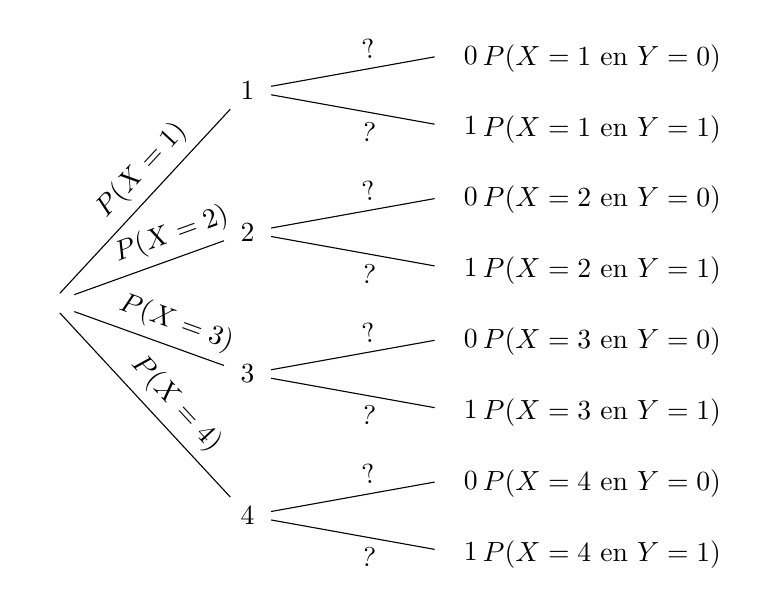
\begin{tikzpicture}[grow=right, sloped]
\node[bag] {}
    child {
        node[bag] {4}        
           child {
                node[end, label=right: {1}] {}
                node[xshift=2.0cm,yshift=-0.04cm] {$P(X=4$ en $Y=1)$}
                edge from parent
                node[below=0cm] {\hspace{0.5cm}?} 
                            }
           child {
                node[end, label=right: {0}] {}
                node[xshift=2.0cm,yshift=-0.04cm] {$P(X=4$ en $Y=0)$}
                edge from parent
                node[above=0cm] {\hspace{0.5cm}?}
                            }
           edge from parent 
           node[above=0cm] {\hspace{0.4cm} $P(X=4)$}
    }
    child {
        node[bag] {3}        
           child {
                node[end, label=right: {1}] {}
                node[xshift=2.0cm,yshift=-0.04cm] {$P(X=3$ en $Y=1)$}
                edge from parent
                node[below=0cm] {\hspace{0.5cm}?}
                            }
           child {
                node[end, label=right: {0}] {}
                node[xshift=2.0cm,yshift=-0.04cm] {$P(X=3$ en $Y=0)$}
                edge from parent
                node[above=0cm] {\hspace{0.5cm}?}
                            }
           edge from parent 
           node[above=0cm] {\hspace{0.4cm} $P(X=3)$}
    }
    child {
        node[bag] {2}        
        child {
             node[end, label=right: {1}] {}
             node[xshift=2.0cm,yshift=-0.04cm] {$P(X=2$ en $Y=1)$}
             edge from parent
             node[below=0cm] {\hspace{0.5cm}?}
                            }
        child {
            node[end, label=right: {0}] {}
             node[xshift=2.0cm,yshift=-0.04cm] {$P(X=2$ en $Y=0)$}
             edge from parent
             node[above=0cm] {\hspace{0.5cm}?}
                            }
        edge from parent 
        node[above=0cm] {\hspace{0.7cm} $P(X=2)$}
    }
    child {
        node[bag] {1}        
           child {
                node[end, label=right: {1}] {}
                node[xshift=2.0cm,yshift=-0.04cm] {$P(X=1$ en $Y=1)$}
                edge from parent
                node[below=0cm] {\hspace{0.5cm}?}
                            }
            child {
                node[end, label=right: {0}] {}
                node[xshift=2.0cm,yshift=-0.04cm] {$P(X=1$ en $Y=0)$}
                edge from parent
                node[above=0cm] {\hspace{0.5cm}?}
                            }
           edge from parent 
           node[above=0cm] {\hspace{0.4cm} $P(X=1)$}
    };
\end{tikzpicture}
\caption{Kansboom bij het kansexperiment over het trekken van een kaart uit een onvolledige set van 10 kaarten met kansen uitgedrukt m.b.v. stochastische veranderlijken}
\label{fig:kaartvb_sv}
\end{afbeeldingenv}
%einde figuur


Ook bij het voorbeeld van de volleybalmatch met de ploeg van Samir kunnen we de kansboom beschrijven met stochastische veranderlijken (zie \autoref{fig:volleybal_sv}). Nu zijn er drie: $X_1$ geeft winnen (1) of verliezen (0) aan voor de ploeg van Samir bij de eerste match, en $X_2$ en $X_3$ geven winnen of verliezen bij de tweede en derde match aan.

%begin figuur
% Set the overall layout of the tree
\tikzstyle{level 1}=[level distance=0.6cm, sibling distance=4cm]
\tikzstyle{level 2}=[level distance=0.6cm, sibling distance=2cm]
\tikzstyle{level 3}=[level distance=0.6cm, sibling distance=1cm]


% Define styles for bags and leafs
\tikzstyle{bag} = [text width=1em, text centered]
\tikzstyle{end} = []
\begin{afbeeldingenv}
\hspace{-1.5cm}$X_1$ \hspace{0.2cm}$X_2$ \hspace{0.3cm} $X_3$ \hspace{0.0cm} spelverloop
\\
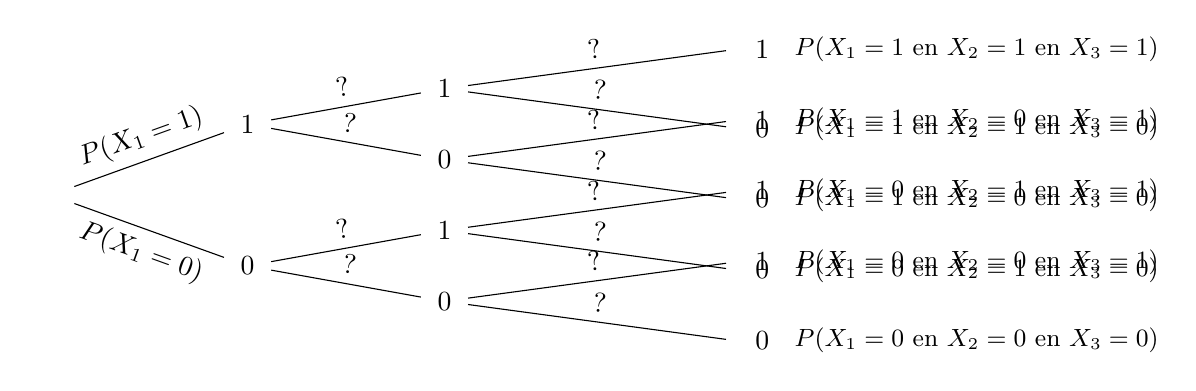
\begin{tikzpicture}[grow=right, sloped]
\node[bag] {}
    child {
        node[bag] {0}        
           child {
                node[bag] {0}
                child {
                    node[end, label=right: {0}] {}
                    node[xshift=0.5cm,yshift=-0cm, label=right: {\small{$P(X_1=0$ en $X_2=0$ en $X_3=0)$}}] {}
                    edge from parent
                    node[above=0cm] {\hspace{0.0cm}?}
                }
                child {
                    node[end, label=right: {1}] {}
                    node[xshift=0.5cm,yshift=-0cm, label=right: {\small{$P(X_1=0$ en $X_2=0$ en $X_3=1)$}}] {}
                    edge from parent
                    node[above=0cm] {\hspace{0.0cm}?}
                }
                edge from parent
                node[above=0cm] {\hspace{0.0cm}?} 
           }
           child {
                node[bag] {1}
                child {
                    node[end, label=right: {0}] {}
                    node[xshift=0.5cm,yshift=-0cm, label=right: {\small{$P(X_1=0$ en $X_2=1$ en $X_3=0)$}}] {}
                    edge from parent
                    node[above=0cm] {\hspace{0.0cm}?}
                }    
                child {
                    node[end, label=right: {1}] {}
                    node[xshift=0.5cm,yshift=-0cm, label=right: {\small{$P(X_1=0$ en $X_2=1$ en $X_3=1)$}}] {}
                    edge from parent
                    node[above=0cm] {\hspace{0.0cm}?}
                }
                edge from parent
                node[above=0cm] {\hspace{0.0cm}?} 
            }
        edge from parent
        node[below=0cm] {\hspace{0.0cm}$P(X_1=0)$} 
    }
    child {
        node[bag] {1}        
           child {
                node[bag] {0}
                child {
                    node[end, label=right: {0}] {}
                    node[xshift=0.5cm,yshift=-0cm, label=right: {\small{$P(X_1=1$ en $X_2=0$ en $X_3=0)$}}] {}
                    edge from parent
                    node[above=0cm] {\hspace{0.0cm}?}
                }
                child {
                    node[end, label=right: {1}] {}
                    node[xshift=0.5cm,yshift=-0cm, label=right: {\small{$P(X_1=1$ en $X_2=0$ en $X_3=1)$}}] {}
                    edge from parent
                    node[above=0cm] {\hspace{0.0cm}?}
                }
                edge from parent
                node[above=0cm] {\hspace{0.0cm}?} 
           }
           child {
                node[bag] {1}
                child {
                    node[end, label=right: {0}] {}
                    node[xshift=0.5cm,yshift=-0cm, label=right: {\small{$P(X_1=1$ en $X_2=1$ en $X_3=0)$}}] {}
                    edge from parent
                    node[above=0cm] {\hspace{0.0cm}?}
                }    
                child {
                    node[end, label=right: {1}] {}
                    node[xshift=0.5cm,yshift=-0cm, label=right: {\small{$P(X_1=1$ en $X_2=1$ en $X_3=1)$}}] {}
                    edge from parent
                    node[above=0cm] {\hspace{0.0cm}?}
                }
                edge from parent
                node[above=0cm] {\hspace{0.0cm}?} 
            }
        edge from parent
        node[above=0cm] {\hspace{0.0cm}$P(X_1=1)$} 
        };
\end{tikzpicture}
\caption{Kansboom bij het volleybalvoorbeeld met kansen uitgedrukt m.b.v. stochastische veranderlijken}
\label{fig:volleybal_sv}
\end{afbeeldingenv}
%einde figuur

\subsection*{Stochastische veranderlijken en verzamelingen}

We hebben de stochastische veranderlijken tot nu toe behandeld op een manier die rechtstreeks aansluit bij de informele behandeling van de kansrekening uit de eerste paragrafen, en die dus los staat van de aanpak met verzamelingen uit \autoref{par:verz}. Het is dus niet per se nodig om eerst de kansrekening met verzamelingen te formuleren om dan later over te stappen op stochastische veranderlijken.

Het is echter ook mogelijk om het begrip stochastische veranderlijke te definiëren vanuit de verzamelingenaanpak van kansruimten. We illustreren dit voor het voorbeeld van de volleybalmatch met de ploeg van Samir:

\begin{itemize}
    \item We letten aanvankelijk nog niet op het aantal keer dat de ploeg van Samir wint. De uitkomsten van het kansexperiment zijn dan 3-tallen: (W, V, V), (V, W, W), \dots Samen vormen ze de uitkomstenverzameling $U$.
    \item De stochastische veranderlijke $X$ die het aantal keer telt dat de ploeg van Samir wint, kunnen we nu beschouwen als een functie van de uitkomstenverzameling $U$ naar $\R$. Zo wordt bijvoorbeeld de uitkomst (W, V, W) door $X$ afgebeeld op het getal $2$.
    \item Met de uitspraak $X=2$ komt de verzameling
    \begin{equation*}
    \begin{split}
     G & =\{u \in U | X(u)=2\} \\
     & =\{(W, W, V),(W, V, W),(V, W, W)\}    
    \end{split}
    \end{equation*}
 overeen.
    \item De kans $P(X=2)$ is gelijk aan $P(G)$.
\end{itemize}
 
\section{Voorwaardelijke kansen}

\subsection*{Voorwaardelijke kansen in een kansboom}

In de vorige paragraaf hebben we gezien dat we de gebeurtenissen en kansen uit een kruistabel kunnen voorstellen met behulp van verzamelingen en van stochastische veranderlijken. Voor kansbomen kon dat maar gedeeltelijk: de kansen langs de takken van de tweede (en eventuele volgende) generatie(s) hebben we nog niet met verzamelingen beschreven. Dat lossen we nu op.

We werken weer met het voorbeeld van het trekken van één kaart uit een set van tien kaarten en kijken naar de kans $0,5$ die bij de bovenste tak van de tweede generatie staat. We kunnen deze kans als volgt omschrijven: het is de kans dat de getrokken kaart een getal bevat als we weten dat het over een schoppen gaat. Meer formeel   wordt zo’n kans een voorwaardelijke kans genoemd. Met de benamingen die we in de vorige paragraaf ingevoerd hebben voor de gebeurtenissen: de kans dat gebeurtenis $G$ zich voordoet, gegeven dat gebeurtenis $S$ zich voorgedaan heeft, genoteerd als $P(G|S)$. In \autoref{fig:kaartvb_voorw} hieronder zie je de kansboom aangevuld met de voorwaardelijke kansen op elk van de takken van de tweede generatie.

\vspace{1cm}

%begin figuur
% Set the overall layout of the tree
\tikzstyle{level 1}=[level distance=2.5cm, sibling distance=2.2cm]
\tikzstyle{level 2}=[level distance=2.5cm, sibling distance=1.1cm]

% Define styles for bags and leafs
\tikzstyle{bag} = [text width=1em, text centered]
\tikzstyle{end} = []

\begin{afbeeldingenv}
\hspace{2.1cm}soort \hspace{1.2cm}getal of figuur?\\
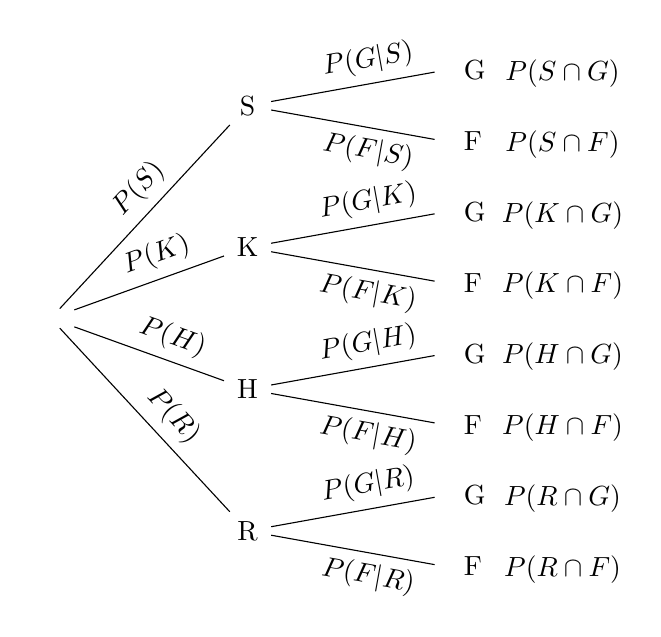
\begin{tikzpicture}[grow=right, sloped]
\node[bag] {}
    child {
        node[bag] {R}        
           child {
                node[end, label=right: {F}] {}
                node[xshift=1.5cm,yshift=-0.04cm] {$P(R \cap F)$}
                edge from parent
                node[below=0cm] {\hspace{0.5cm}$P(F|R)$} 
                            }
           child {
                node[end, label=right: {G}] {}
                node[xshift=1.5cm,yshift=-0.04cm] {$P(R \cap G)$}
                edge from parent
                node[above=0cm] {\hspace{0.5cm}$P(G|R)$}
                            }
           edge from parent 
           node[above=0cm] {\hspace{0.3cm} $P(R)$}
    }
    child {
        node[bag] {H}        
           child {
                node[end, label=right: {F}] {}
                node[xshift=1.5cm,yshift=-0.04cm] {$P(H \cap F)$}
                edge from parent
                node[below=0cm] {\hspace{0.5cm}$P(F|H)$}
                            }
           child {
                node[end, label=right: {G}] {}
                node[xshift=1.5cm,yshift=-0.04cm] {$P(H \cap G)$}
                edge from parent
                node[above=0cm] {\hspace{0.5cm}$P(G|H)$}
                            }
           edge from parent 
           node[above=0cm] {\hspace{0.3cm} $P(H)$}
    }
    child {
        node[bag] {K}        
           child {
                node[end, label=right: {F}] {}
                node[xshift=1.5cm,yshift=-0.04cm] {$P(K \cap F)$}
                edge from parent
                node[below=0cm] {\hspace{0.5cm}$P(F|K)$}
                            }
            child {
                node[end, label=right: {G}] {}
                node[xshift=1.5cm,yshift=-0.04cm] {$P(K \cap G)$}
                edge from parent
                node[above=0cm] {\hspace{0.5cm}$P(G|K)$}
                            }
           edge from parent 
           node[above=0cm] {\hspace{0.3cm} $P(K)$}
    }
    child {
        node[bag] {S}        
           child {
                node[end, label=right: {F}] {}
                node[xshift=1.5cm,yshift=-0.04cm] {$P(S \cap F)$}
                edge from parent
                node[below=0cm] {\hspace{0.5cm}$P(F|S)$}
                            }
            child {
                node[end, label=right: {G}] {}
                node[xshift=1.5cm,yshift=-0.04cm] {$P(S \cap G)$}
                edge from parent
                node[above=0cm] {\hspace{0.5cm}$P(G|S)$}
                            }
           edge from parent 
           node[above=0cm] {\hspace{0.3cm} $P(S)$}
    };
\end{tikzpicture}
\caption{Kansboom bij het kansexperiment over het
trekken van een kaart uit een onvolledige set van 10 kaarten aangevuld met voorwaardelijke kansen}
\label{fig:kaartvb_voorw}
\end{afbeeldingenv}
%einde figuur
%\vspace{0.5cm}

In de vorige paragraaf hebben we besproken dat het feit dat de som van $P(S)$, $P(K)$, $P(H)$ en $P(R)$ gelijk is aan $1$ een gevolg is van het feit dat $S$, $K$, $H$ en $R$ een partitie van het universum $U$ vormen. Voor de takken van de tweede generatie geldt iets gelijkaardigs. Bijvoorbeeld: de voorwaardelijke kansen bij de twee takken die uit de knoop $S$ vertrekken hebben als som $1$. Dit is gemakkelijk in te zien in formulevorm:
%\vspace{0.5cm}

\begin{equation*}
\begin{split}
P(G|S)+P(F|S) & =\frac{P(S \cap G)}{P(S)}+\frac{P(S \cap F)}{P(S)} \\
 & =\frac{P(S \cap G)+P(S \cap F)}{P(S)} \\
 & =\frac{P(S)}{P(S)} \\
 & =1
\end{split}
\end{equation*}
%\vspace{0.5cm}


Dat hangt samen met het feit dat de gebeurtenissen bij de overeenkomstige twee bladeren, namelijk $S \cap G$ en $S \cap F$, een partitie vormen van $S$. 

We gebruiken analoge benamingen en notaties bij stochastische veranderlijken: $P(Y=0 | X=1)$ is de kans dat $Y$ de waarde $0$ aanneemt, gegeven dat $X$ de waarde $1$ aanneemt. De overeenkomstige kansboom vind je in \autoref{fig:kaart_sv_voorw}.
\vspace{0.5cm}

%begin figuur
% Set the overall layout of the tree
\tikzstyle{level 1}=[level distance=1.7cm, sibling distance=2.2cm]
\tikzstyle{level 2}=[level distance=2.5cm, sibling distance=1.1cm]

% Define styles for bags and leafs
\tikzstyle{bag} = [text width=1em, text centered]
\tikzstyle{end} = []

\begin{afbeeldingenv}
\hspace{-0.3cm}X \hspace{2.5cm}Y\\
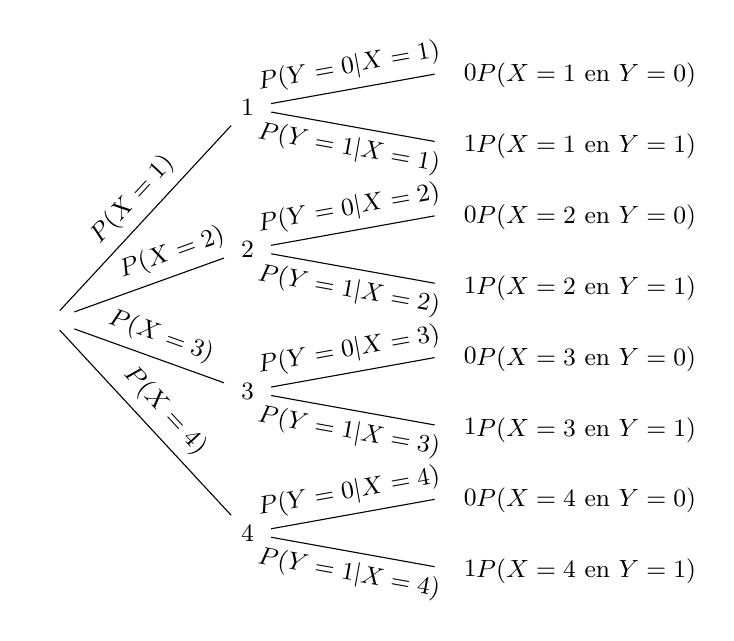
\begin{tikzpicture}[grow=right, sloped]
\node[bag] {}
    child {
        node[bag] {\small{4}}        
           child {
                node[end, label=right: {\small{1}}] {}
                node[xshift=1.8cm,yshift=-0.04cm] {\small{$P(X=4$ en $Y=1)$}}
                edge from parent
                node[below=0cm] {\small{$P(Y=1|X=4)$}} 
                            }
           child {
                node[end, label=right: {\small{0}}] {}
                node[xshift=1.8cm,yshift=-0.04cm] {\small{$P(X=4$ en $Y=0)$}}
                edge from parent
                node[above=0cm] {\small{$P(Y=0|X=4)$}}
                            }
           edge from parent 
           node[above=0cm] {\hspace{0.0cm} \small{$P(X=4)$}}
    }
    child {
        node[bag] {\small{3}}        
           child {
                node[end, label=right: {\small{1}}] {}
                node[xshift=1.8cm,yshift=-0.04cm] {\small{$P(X=3$ en $Y=1)$}}
                edge from parent
                node[below=0cm] {\small{$P(Y=1|X=3)$}}
                            }
           child {
                node[end, label=right: {\small{0}}] {}
                node[xshift=1.8cm,yshift=-0.04cm] {\small{$P(X=3$ en $Y=0)$}}
                edge from parent
                node[above=0cm] {\small{$P(Y=0|X=3)$}}
                            }
           edge from parent 
           node[above=0cm] {\hspace{0.0cm} \small{$P(X=3)$}}
    }
    child {
        node[bag] {\small{2}}        
           child {
                node[end, label=right: {\small{1}}] {}
                node[xshift=1.8cm,yshift=-0.04cm] {\small{$P(X=2$ en $Y=1)$}}
                edge from parent
                node[below=0cm] {\small{$P(Y=1|X=2)$}}
                            }
            child {
                node[end, label=right: {\small{0}}] {}
                node[xshift=1.8cm,yshift=-0.04cm] {\small{$P(X=2$ en $Y=0)$}}
                edge from parent
                node[above=0cm] {\small{$P(Y=0|X=2)$}}
                            }
           edge from parent 
           node[above=0cm] {\hspace{0.7cm} \small{$P(X=2)$}}
    }
    child {
        node[bag] {\small{1}}        
           child {
                node[end, label=right: {\small{1}}] {}
                node[xshift=1.8cm,yshift=-0.04cm] {\small{$P(X=1$ en $Y=1)$}}
                edge from parent
                node[below=0cm] {\small{$P(Y=1|X=1)$}}
                            }
            child {
                node[end, label=right: {\small{0}}] {}
                node[xshift=1.8cm,yshift=-0.04cm] {\small{$P(X=1$ en $Y=0)$}}
                edge from parent
                node[above=0cm] {\small{$P(Y=0|X=1)$}}
                            }
           edge from parent 
           node[above=0cm] {\hspace{0.0cm} \small{$P(X=1)$}}
    };
\end{tikzpicture}
\caption{Kansboom bij het kansexperiment over het
trekken van een kaart uit een onvolledige set van 10 kaarten aangevuld met voorwaardelijke kansen uitgedrukt m.b.v. stochastische veranderlijken}
\label{fig:kaart_sv_voorw}
\end{afbeeldingenv}
%einde figuur
\vspace{0.5cm}

Als het kansexperiment uiteenvalt in meer dan twee deelexperimenten, zoals in het voorbeeld van de volleybalmatch met de ploeg van Samir, zijn ook de kansen op de takken van de derde en eventuele volgende generaties voorwaardelijke kansen. Zo is hier bijvoorbeeld de kans bij de bovenste tak van de derde generatie de voorwaardelijke kans $P(X_3=1|X_1=1$ en $X_2=1)$ (zie \autoref{fig:volleybal_sv_voorw}).

\newpage

%begin figuur
% Set the overall layout of the tree
\tikzstyle{level 1}=[level distance=0.5cm, sibling distance=4cm]
\tikzstyle{level 2}=[level distance=2.4cm, sibling distance=2cm]
\tikzstyle{level 3}=[level distance=3.7cm, sibling distance=1cm]


% Define styles for bags and leafs
\tikzstyle{bag} = [text width=1em, text centered]
\tikzstyle{end} = []

\begin{afbeeldingenv}
\hspace{0.61cm}$X_1$ \hspace{2.1cm}$X_2$ \hspace{3.4cm} $X_3$
\\
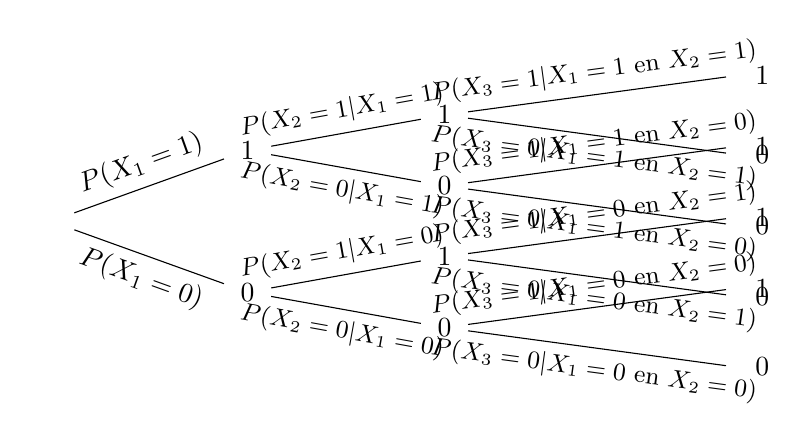
\begin{tikzpicture}[grow=right, sloped]
\node[bag] {}
    child {
        node[bag] {0}        
           child {
                node[bag] {0}
                child {
                    node[end, label=right: {0}] {}
                    edge from parent
                    node[below=0cm, ] {\hspace{0.0cm}\small{$P(X_3=0|X_1=0$ en $X_2=0)$}}
                }
                child {
                    node[end, label=right: {1}] {}
                    edge from parent
                    node[above=0cm] {\hspace{0.0cm}\small{$P(X_3=1|X_1=0$ en $X_2=0)$}}
                }
                edge from parent
                node[below=0cm] {\hspace{0.0cm}\small{$P(X_2=0|X_1=0)$}} 
           }
           child {
                node[bag] {1}
                child {
                    node[end, label=right: {0}] {}
                    edge from parent
                    node[below=0cm] {\hspace{0.0cm}\small{$P(X_3=0|X_1=0$ en $X_2=1)$}}
                }    
                child {
                    node[end, label=right: {1}] {}
                    edge from parent
                    node[above=0cm] {\hspace{0.0cm}\small{$P(X_3=1|X_1=0$ en $X_2=1)$}}
                }
                edge from parent
                node[above=0cm] {\hspace{0.0cm}\small{$P(X_2=1|X_1=0)$}} 
            }
        edge from parent
        node[below=0cm] {\hspace{0.0cm}$P(X_1=0)$} 
    }
    child {
        node[bag] {1}        
           child {
                node[bag] {0}
                child {
                    node[end, label=right: {0}] {}
                    edge from parent
                    node[below=0cm] {\hspace{0.0cm}\small{$P(X_3=0|X_1=1$ en $X_2=0)$}}
                }
                child {
                    node[end, label=right: {1}] {}
                    edge from parent
                    node[above=0cm] {\hspace{0.0cm}\small{$P(X_3=1|X_1=1$ en $X_2=0)$}}
                }
                edge from parent
                node[below=0cm] {\hspace{0.0cm}\small{$P(X_2=0|X_1=1)$}} 
           }
           child {
                node[bag] {1}
                child {
                    node[end, label=right: {0}] {}
                    edge from parent
                    node[below=0cm] {\hspace{0.0cm}\small{$P(X_3=0|X_1=1$ en $X_2=1)$}}
                }    
                child {
                    node[end, label=right: {1}] {}
                    edge from parent
                    node[above=0cm] {\hspace{0.0cm}\small{$P(X_3=1|X_1=1$ en $X_2=1)$}}
                }
                edge from parent
                node[above=0cm] {\hspace{0.0cm}\small{$P(X_2=1|X_1=1)$} }
            }
        edge from parent
        node[above=0cm] {\hspace{0.0cm}$P(X_1=1)$} 
        };
\end{tikzpicture}
\caption{Kansboom bij het volleybalvoorbeeld aangevuld met voorwaardelijke kansen uitgedrukt m.b.v. stochastische veranderlijken}
\label{fig:volleybal_sv_voorw}
\end{afbeeldingenv}
%einde figuur

\subsection*{De productregel}
Met dit nieuwe begrip voorwaardelijke kans kunnen we de productregel (‘om de kans van een blad te vinden, moet je het product maken van de kansen langs de takken die naar dit blad leiden’) nu in formulevorm weergeven. In het kaartvoorbeeld komt de productregel voor de kans bij het bovenste blad (zie \autoref{fig:kaartvb_voorw}) bijvoorbeeld neer op:
$$P(S \cap G)=P(S) \cdot P(G|S).$$
Dit geldt algemeen: 
\begin{kader}{Eigenschap}{Productregel}
Als $A$ en $B$ twee gebeurtenissen zijn, dan is
$$P(A \cap B)=P(A) \cdot P(B|A).$$
\end{kader}

\subsection*{Definitie van een voorwaardelijke kans met verzamelingen en met stochastische veranderlijken}

Als we in de productregel hierboven beide leden delen door $P(A)$, dan krijgen we de definitie van een voorwaardelijke kans in termen van verzamelingen:

\begin{kader}{Definitie}{Voorwaardelijke kans}
De kans dat gebeurtenis $B$ zich voordoet gegeven dat gebeurtenis $A$ zich voorgedaan heeft, is
$$P(B|A)=\frac {P(A \cap B)} {P(A)}.$$
\end{kader}

Dit laat zich onmiddellijk vertalen naar stochastische veranderlijken:
$$P(X_2=x_2|X_1=x_1)=\frac {P(X_1=x_1 \text{ en } X_2=x_2)} {P(X_1=x_1)}.$$

\subsection*{Voorwaardelijke kansen in kruistabellen}

In een kruistabel komen geen voorwaardelijke kansen voor. De kansen die je nodig hebt om deze voorwaardelijke kansen te berekenen, vind je wel in de kruistabel. Bijvoorbeeld: om in het kaartvoorbeeld een voorwaardelijke kans als $P(G|S)$ te berekenen, vind je de teller in het ‘midden’ van de kruistabel en de noemer als een van de marginale kansen:
$$P(G|S)=\frac {P(G \cap S)} {P(S)} = \frac {0,1} {0,2}=0,5.$$

\subsection*{Kansboom of kruistabel?}

We hebben ondertussen vastgesteld dat we in een kruistabel andere kansen voorstellen dan in een kansboom. Welk van beide voorstellingen het handigste is om te gebruiken, hangt af van het gestelde probleem. Als er drie of meer deelexperimenten zijn, dan kan het niet met een kruistabel omdat die slechts twee ‘dimensies’ heeft. 

Als er twee deelexperimenten zijn, dan zijn beide voorstellingen mogelijk. In sommige kansproblemen krijgen we precies de kansen die we nodig hebben om de kansboom op te stellen. Dit is bijvoorbeeld het geval in het voorbeeld van het testen op een bepaalde ziekte uit \autoref{par:valspos}. Het opstellen van de kruistabel vereist hier wat meer rekenwerk. In andere situaties sluit een kruistabel dan weer beter aan bij de gegeven kansen. Of het kan ook gebeuren dat niet de gegeven kansen, maar de gevraagde kans zich beter leent voor een kansboom dan wel een kruistabel.

De ene keer is dus een kansboom meer aangewezen, en een andere keer is de kruistabel handiger. Het blijft weliswaar relatief: als je een probleem met een kansboom kunt oplossen, dan gaat het ook met een kruistabel, en omgekeerd. Je kunt dus ook wel je persoonlijke voorkeur laten spelen.

\subsection*{De regel van Bayes met verzamelingen}

We keren terug naar het voorbeeld van het trekken van één kaart uit een set van tien kaarten. We vragen ons af wat de kans is dat de getrokken kaart een schoppen is als we al weten dat er een getal op de kaart staat. De gevraagde kans is een voorwaardelijke kans: $P(S|G)$. Als we deze kans vergelijken met $P(G|S)$, een van de kansen die we in onze kansboom gebruikten (zie \autoref{fig:kaartvb_voorw}), dan zien we dat het in beide gevallen over voorwaardelijke kansen gaat, waarin bovendien dezelfde gebeurtenissen optreden, maar waarin de rollen van de gebeurtenissen omgewisseld zijn: in de kans uit de kansboom gaan we ervan uit dat we weten dat het om een schoppen gaat, en in de gevraagde kans gaan we ervan uit dat we weten dat het over een kaart met een getal gaat.

Dit omwisselen van de rollen in een voorwaardelijke kans is typisch voor problemen in de kansrekening. We hebben het in een meer betekenisvolle context al ontmoet bij het voorbeeld van het testen op een bepaalde ziekte uit \autoref{par:valspos}. In zo’n situatie zijn we typisch geïnteresseerd in de kans dat we daadwerkelijk ziek zijn als de test positief uitvalt, terwijl de gegeven voorwaardelijke kansen betrekking hebben op het al dan niet positief zijn van de test bij zieke en gezonde personen. 
\vspace{0.5cm}

%begin figuur
% Set the overall layout of the tree
\tikzstyle{level 1}=[level distance=2.5cm, sibling distance=1.5cm]
\tikzstyle{level 2}=[level distance=2.5cm, sibling distance=0.75cm]

% Define styles for bags and leafs
\tikzstyle{bag} = [text width=1em, text centered]
\tikzstyle{end} = []

\begin{afbeeldingenv}
\hspace{2.4cm}soort \hspace{1.2cm}getal of figuur?\\
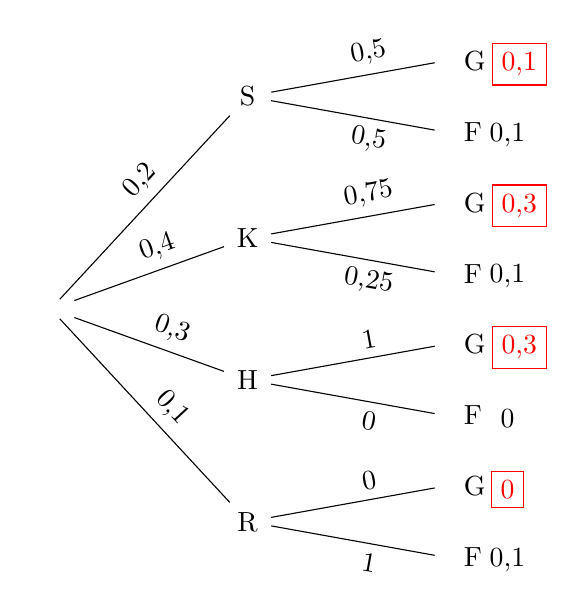
\begin{tikzpicture}[grow=right, sloped]
\node[bag] {}
    child {
        node[bag] {R}        
           child {
                node[end, label=right: {F}] {}
                node[xshift=0.8cm,yshift=-0.04cm] {0,1}
                edge from parent
                node[below=0cm] {\hspace{0.5cm}1} 
                            }
           child {
                node[end, label=right: {G}] {}
                node[rectangle,draw,xshift=0.8cm,yshift=-0.04cm, red] {0}
                edge from parent
                node[above=0cm] {\hspace{0.5cm}0}
                            }
           edge from parent 
           node[above=0cm] {\hspace{0.3cm} 0,1}
    }
    child {
        node[bag] {H}        
           child {
                node[end, label=right: {F}] {}
                node[xshift=0.8cm,yshift=-0.04cm] {0}
                edge from parent
                node[below=0cm] {\hspace{0.5cm}0}
                            }
           child {
                node[end, label=right: {G}] {}
                node[rectangle,draw,xshift=0.95cm,yshift=-0.04cm,red] {0,3}
                edge from parent
                node[above=0cm] {\hspace{0.5cm}1}
                            }
           edge from parent 
           node[above=0cm] {\hspace{0.3cm} 0,3}
    }
    child {
        node[bag] {K}        
           child {
                node[end, label=right: {F}] {}
                node[xshift=0.8cm,yshift=-0.04cm] {0,1}
                edge from parent
                node[below=0cm] {\hspace{0.5cm}0,25}
                            }
            child {
                node[end, label=right: {G}] {}
                node[rectangle,draw,xshift=0.95cm,yshift=-0.04cm,red] {0,3}
                edge from parent
                node[above=0cm] {\hspace{0.5cm}0,75}
                            }
           edge from parent 
           node[above=0cm] {\hspace{0.3cm} 0,4}
    }
    child {
        node[bag] {S}        
           child {
                node[end, label=right: {F}] {}
                node[xshift=0.8cm,yshift=-0.04cm] {0,1}
                edge from parent
                node[below=0cm] {\hspace{0.5cm}0,5}
                            }
            child {
                node[end, label=right: {G}] {}
                node[rectangle,draw,xshift=0.95cm,yshift=-0.04cm,red] {0,1}
                edge from parent
                node[above=0cm] {\hspace{0.5cm}0,5}
                            }
           edge from parent 
           node[above=0cm] {\hspace{0.3cm} 0,2}
    };
\end{tikzpicture}
\caption{Kansboom bij het kaartvoorbeeld met kansen aangeduid die je gebruikt bij het berekenen van $P(S|G)$}
\label{kaartvb_Bayes}
\end{afbeeldingenv}
%einde figuur

In het eerste deel van de loep hebben we gezien hoe we dergelijke kansen louter met ons gezond verstand kunnen uitrekenen door gebruik te maken van de kansen die op het einde van de kansboom verschijnen (zie \autoref{kaartvb_Bayes} hierboven). Ook met de kansboom van het kaartvoorbeeld kunnen we dit eenvoudig doen door er de gepaste bladeren uit te kiezen:

\vspace{0.3cm}
$$P(S|G)=\frac{0,1}{0,1+0,3+0,3+0}=\frac{1}{7}.$$
\vspace{0.3cm}


Deze informele oplossing kunnen we als volgt met verzamelingen formuleren (zie \autoref{fig:kaartvb_Bayes_verz}):
\vspace{0.3cm}
$$P(S|G)=\frac {P(S \cap G)} {P(S\cap G)+P(K \cap G)+P(H \cap G)+P(R \cap G)}$$
\vspace{0.3cm}

of, met de productregel:

\vspace{0.3cm}
$$P(S|G)=\frac {P(S) \cdot P(G|S)} {P(S) \cdot P(G|S)+...+P(R) \cdot P(G|R)}.$$
\vspace{0.3cm}

%begin figuur
% Set the overall layout of the tree
\tikzstyle{level 1}=[level distance=2.5cm, sibling distance=1.8cm]
\tikzstyle{level 2}=[level distance=2.5cm, sibling distance=0.9cm]

% Define styles for bags and leafs
\tikzstyle{bag} = [text width=1em, text centered]
\tikzstyle{end} = []

\begin{afbeeldingenv}
\hspace{2.4cm}soort \hspace{1.2cm}getal of figuur?\\
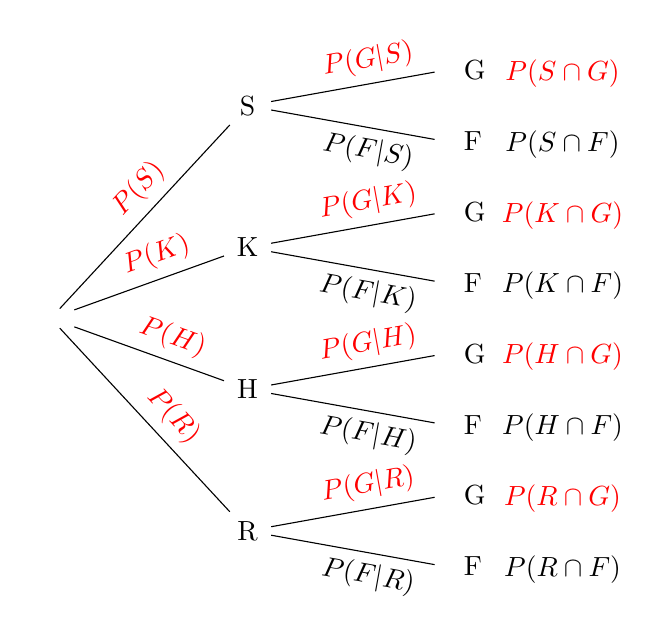
\begin{tikzpicture}[grow=right, sloped]
\node[bag] {}
    child {
        node[bag] {R}        
           child {
                node[end, label=right: {F}] {}
                node[xshift=1.5cm,yshift=-0.04cm] {$P(R \cap F)$}
                edge from parent
                node[below=0cm] {\hspace{0.5cm}$P(F|R)$} 
                            }
           child {
                node[end, label=right: {G}] {}
                node[xshift=1.5cm,yshift=-0.04cm, red] {$P(R \cap G)$}
                edge from parent
                node[above=0cm,red] {\hspace{0.5cm}$P(G|R)$}
                            }
           edge from parent 
           node[above=0cm,red] {\hspace{0.3cm} $P(R)$}
    }
    child {
        node[bag] {H}        
           child {
                node[end, label=right: {F}] {}
                node[xshift=1.5cm,yshift=-0.04cm] {$P(H \cap F)$}
                edge from parent
                node[below=0cm] {\hspace{0.5cm}$P(F|H)$}
                            }
           child {
                node[end, label=right: {G}] {}
                node[xshift=1.5cm,yshift=-0.04cm,red] {$P(H \cap G)$}
                edge from parent
                node[above=0cm,red] {\hspace{0.5cm}$P(G|H)$}
                            }
           edge from parent 
           node[above=0cm,red] {\hspace{0.3cm} $P(H)$}
    }
    child {
        node[bag] {K}        
           child {
                node[end, label=right: {F}] {}
                node[xshift=1.5cm,yshift=-0.04cm] {$P(K \cap F)$}
                edge from parent
                node[below=0cm] {\hspace{0.5cm}$P(F|K)$}
                            }
            child {
                node[end, label=right: {G}] {}
                node[xshift=1.5cm,yshift=-0.04cm,red] {$P(K \cap G)$}
                edge from parent
                node[above=0cm,red] {\hspace{0.5cm}$P(G|K)$}
                            }
           edge from parent 
           node[above=0cm,red] {\hspace{0.3cm} $P(K)$}
    }
    child {
        node[bag] {S}        
           child {
                node[end, label=right: {F}] {}
                node[xshift=1.5cm,yshift=-0.04cm] {$P(S \cap F)$}
                edge from parent
                node[below=0cm] {\hspace{0.5cm}$P(F|S)$}
                            }
            child {
                node[end, label=right: {G}] {}
                node[xshift=1.5cm,yshift=-0.04cm,red] {$P(S \cap G)$}
                edge from parent
                node[above=0cm,red] {\hspace{0.5cm}$P(G|S)$}
                            }
           edge from parent 
           node[above=0cm,red] {\hspace{0.3cm} $P(S)$}
    };
\end{tikzpicture}
\caption{Kansboom bij het kaartvoorbeeld met kansen  die je gebruikt bij het berekenen van $P(S|G)$ aangeduid in termen van gebeurtenissen}
\label{fig:kaartvb_Bayes_verz}
\end{afbeeldingenv}
%einde figuur

\newpage
In het algemeen geformuleerd is dit een van de vormen van de stelling van Bayes:

\vspace{0.5cm}
\begin{kader}{Eigenschap}{Stelling van Bayes}
Stel dat $B$ een gebeurtenis is, en dat $A_1$, $A_2$, \dots, $A_n$ twee aan twee disjuncte gebeurtenissen zijn waarvan de unie gelijk is aan het universum $U$ (met andere woorden: stel dat $A_1$, $A_2$, …, $A_n$ een partitie van $U$ vormen), dan is
\small{$$P(A_1|B)=\frac {P(A_1) \cdot P(B|A_1)} {(P(A_1) \cdot P(B|A_1)+ \cdots +P(A_n) \cdot P(B|A_n)}.$$}
\begin{afbeeldingenv}
\includestandalone{img/bayesboomtikztje.tex}
\end{afbeeldingenv}
\end{kader}
%\vspace{0.3cm}


We kunnen de stelling van Bayes nog in een andere vorm formuleren: de noemer in bovenstaande formule is immers niets anders dan de (‘totale’) kans van gebeurtenis $B$. We krijgen dus:
\vspace{0.5cm}
$$P(A_1|B)=\frac {P(A_1)}{P(B)} \cdot P(B|A_1).$$
\vspace{-0.5cm}

In deze vorm zien we het omwisselen van de voorwaardelijkheid in de kansen heel duidelijk naar voor komen. Je kunt deze korte formule overigens ook rechtstreeks afleiden door de voorwaardelijke kans uit het linkerlid uit te schrijven met de definitie, in combinatie met de productregel voor de kans van de doorsnede:
%\vspace{0.3cm}

\begin{equation*}
\begin{split}
P(A_1|B) & =\frac {P(A_1 \cap B)} {P(B)} \\
 & = \frac {P(A_1) \cdot P(B|A_1)} {P(B)} \\
 & = \frac {P(A_1)} {P(B)} \cdot P(B|A_1)
\end{split}
\end{equation*}
Voor een wat gedetailleerder uitwerking van de overgang van informeel naar formeel werken rond de stelling van Bayes verwijzen we naar (Tytgat, 2002).

\subsection*{Voorwaardelijke kans en kans op de doorsnede}

Wanneer leerlingen een probleem dat in woorden gesteld is, moeten vertalen naar kansen, verwarren ze de onderstaande kansen vaak met elkaar:
\begin {itemize}
    \item de voorwaardelijke kans $P(B|A)$: de kans dat $B$ zich voordoet, gegeven dat $A$ zich voorgedaan heeft;
    \item $P(B)$: de ‘onvoorwaardelijke’ kans van $B$;
    \item $P(A \cap B)$: de kans dat $A$ en $B$ zich beide voordoen;
    \item $P(A|B)$: de voorwaardelijke kans met $A$ en $B$ in de omgekeerde rol.
\end{itemize}
Daarom is het goed om dit onderscheid in te oefenen en hieromtrent ‘vertaaloefeningen’ te maken. Vraag bijvoorbeeld om de onderstaande zinnen (over het bestand aan appartementen in een stad) te vertalen in een kans die in symbolen weergegeven is (het kansexperiment is het lukraak kiezen van een appartement):
\begin{itemize}
    \item 20\% van de appartementen met uitzicht op de rivier heeft drie slaapkamers;
    \item 20\% van de appartementen heeft drie slaapkamers;
    \item 20\% van de appartementen heeft drie slaapkamers en uitzicht op de rivier;
    \item 20\% van de appartementen met drie slaapkamers heeft uitzicht op de rivier.
\end{itemize}
Je kunt de vertaling ook in de omgekeerde richting laten maken. Je omschrijft dan zelf gebeurtenissen en vraagt om kansen in zinnen te vertalen.

\section{Onafhankelijkheid}

\subsection*{Trekken met en zonder teruglegging: (on)afhankelijke gebeurtenissen in kansbomen}

Uit een vaas met twee blauwe, drie rode en vier witte ballen trekken we achtereenvolgens twee ballen.

We kunnen de uitkomsten voorstellen als koppels. Zo noteren we (W, R) om aan te geven dat er eerst een witte bal getrokken werd en vervolgens een rode. De gebeurtenis ‘de eerste bal is blauw’, bijvoorbeeld, is dan de verzameling $B_1=\{$(B, B),(B, R),(B, W)$\}$.

Je kunt dit kansexperiment in twee varianten uitvoeren: met of zonder teruglegging. In een kansboom krijgen we voor beide varianten dezelfde boomstructuur maar met andere kansen op de takken die bij de tweede trekking horen (zie \autoref{fig:ballen_zonder}
 en \autoref{fig:ballen_met}).


In de versie zonder teruglegging, zien we dat de kansen op de vervolgtakken beïnvloed worden door wat er uit de eerste trekking gekomen is. Zo is bijvoorbeeld (zie de rode kansen in \autoref{fig:ballen_zonder})
\begin{equation*}
\begin{split}
P(\text{tw} & \text{eede bal is blauw | eerste bal is blauw})= \\
 & = P(B_2|B_1)=\frac{1}{8},
\end{split}
\end{equation*}
(want er zit maar één blauwe bal meer in de vaas) terwijl
\begin{equation*}
\begin{split}
P(\text{tw} & \text{eede bal is blauw | eerste bal is rood})= \\
 & = P(B_2|R_1)=\frac{2}{8},
\end{split}
\end{equation*}
\begin{equation*}
\begin{split}
P(\text{tw} & \text{eede bal is blauw | eerste bal is wit})= \\
 & = P(B_2|W_1)=\frac{2}{8}.
\end{split}
\end{equation*}
We spreken in dit geval van \emph{afhankelijkheid}: de kansen bij de tweede trekking hangen af van de kleur die in eerste trekking naar boven gekomen is. We houden de formulering bewust nog vaag, maar zullen ze verderop precies maken.

In de variant met teruglegging treedt dit fenomeen niet op: daar zijn de bovenstaande drie kansen alle drie gelijk aan $2/9$. De kansen op de vervolgtakken worden hier niet beïnvloed door wat er uit de eerste trekking gekomen is. Logisch, want we leggen de getrokken bal terug. In dit geval spreken we over \emph{onafhankelijkheid}.


%begin figuur zonder teruglegging
% Set the overall layout of the tree
\tikzstyle{level 1}=[level distance=2.5cm, sibling distance=2.4cm]
\tikzstyle{level 2}=[level distance=2.5cm, sibling distance=0.8cm]

% Define styles for bags and leafs
\tikzstyle{bag} = [text width=3em, text centered]
\tikzstyle{end} = [circle, minimum width=0pt,fill, inner sep=0pt]

\begin{afbeeldingenv}
\hspace{2.6cm}1ste bal \hspace{1.8cm}2de bal\\
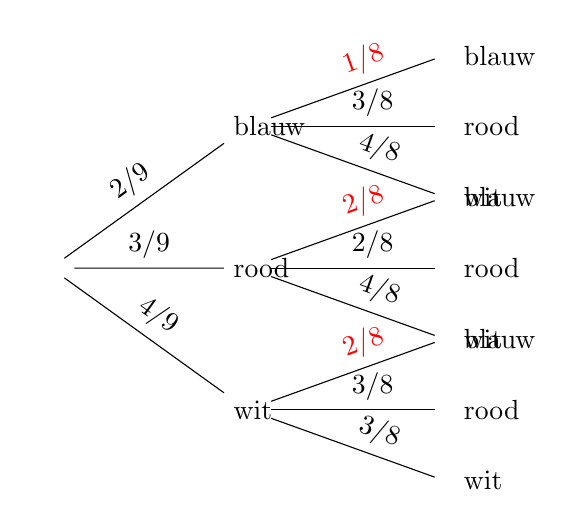
\begin{tikzpicture}[grow=right, sloped]
\node[bag] {}
    child {
        node[bag] {wit}        
           child {
                node[end, label=right: {wit}] {}
                edge from parent
                node[above=0cm] {\hspace{0.5cm}3/8}
                            }
           child {
                node[end, label=right: {rood}] {}
                edge from parent
                node[above=0cm] {\hspace{0.5cm}3/8}
                            }
           child {
                node[end, label=right: {blauw}] {}
                edge from parent
                node[above=0cm,red] {\hspace{0.5cm}2/8}
                            }
           edge from parent 
           node[above=0cm] {\hspace{0.0cm}4/9}
    }
    child {
        node[bag] {rood}        
           child {
                node[end, label=right: {wit}] {}
                edge from parent
                node[above=0cm] {\hspace{0.5cm}4/8}
                            }
           child {
                node[end, label=right: {rood}] {}
                edge from parent
                node[above=0cm] {\hspace{0.5cm}2/8}
                            }
           child {
                node[end, label=right: {blauw}] {}
                edge from parent
                node[above=0cm,red] {\hspace{0.5cm}2/8}
                            }
           edge from parent 
           node[above=0cm] {\hspace{0.0cm}3/9}
    }
    child {
        node[bag] {blauw}        
           child {
                node[end, label=right: {wit}] {}
                edge from parent
                node[above=0cm] {\hspace{0.5cm}4/8}
                            }
           child {
                node[end, label=right: {rood}] {}
                edge from parent
                node[above=0cm] {\hspace{0.5cm}3/8}
                            }
           child {
                node[end, label=right: {blauw}] {}
                edge from parent
                node[above=0cm,red] {\hspace{0.5cm}1/8}
                            }
           edge from parent 
           node[above=0cm] {\hspace{0.0cm}2/9}
    };
\end{tikzpicture}
\caption{Kansboom bij het trekken van twee ballen zonder terugleggen}
\label{fig:ballen_zonder}
\end{afbeeldingenv}
%einde figuur zonder teruglegging



%begin figuur met teruglegging
% Set the overall layout of the tree
\tikzstyle{level 1}=[level distance=2.5cm, sibling distance=2.4cm]
\tikzstyle{level 2}=[level distance=2.5cm, sibling distance=0.8cm]

% Define styles for bags and leafs
\tikzstyle{bag} = [text width=3em, text centered]
\tikzstyle{end} = [circle, minimum width=0pt,fill, inner sep=0pt]

\begin{afbeeldingenv}
\hspace{2.6cm}1ste bal \hspace{1.8cm}2de bal\\
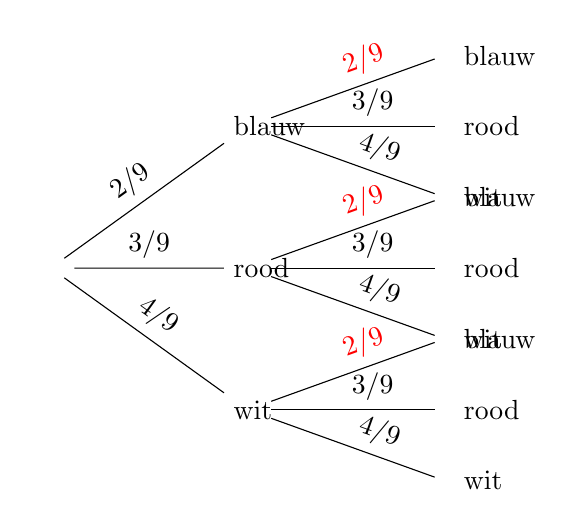
\begin{tikzpicture}[grow=right, sloped]
\node[bag] {}
    child {
        node[bag] {wit}        
           child {
                node[end, label=right: {wit}] {}
                edge from parent
                node[above=0cm] {\hspace{0.5cm}4/9}
                            }
           child {
                node[end, label=right: {rood}] {}
                edge from parent
                node[above=0cm] {\hspace{0.5cm}3/9}
                            }
           child {
                node[end, label=right: {blauw}] {}
                edge from parent
                node[above=0cm,red] {\hspace{0.5cm}2/9}
                            }
           edge from parent 
           node[above=0cm] {\hspace{0.0cm}4/9}
    }
    child {
        node[bag] {rood}        
           child {
                node[end, label=right: {wit}] {}
                edge from parent
                node[above=0cm] {\hspace{0.5cm}4/9}
                            }
           child {
                node[end, label=right: {rood}] {}
                edge from parent
                node[above=0cm] {\hspace{0.5cm}3/9}
                            }
           child {
                node[end, label=right: {blauw}] {}
                edge from parent
                node[above=0cm,red] {\hspace{0.5cm}2/9}
                            }
           edge from parent 
           node[above=0cm] {\hspace{0.0cm}3/9}
    }
    child {
        node[bag] {blauw}        
           child {
                node[end, label=right: {wit}] {}
                edge from parent
                node[above=0cm] {\hspace{0.5cm}4/9}
                            }
           child {
                node[end, label=right: {rood}] {}
                edge from parent
                node[above=0cm] {\hspace{0.5cm}3/9}
                            }
           child {
                node[end, label=right: {blauw}] {}
                edge from parent
                node[above=0cm,red] {\hspace{0.5cm}2/9}
                            }
           edge from parent 
           node[above=0cm] {\hspace{0.0cm}2/9}
    };
\end{tikzpicture}
\caption{Kansboom bij het trekken van twee ballen met terugleggen}
\label{fig:ballen_met}
\end{afbeeldingenv}
%einde figuur met teruglegging




In de variant met teruglegging is $P(B_2)$, de ‘totale’ kans dat de tweede bal blauw is, gelijk aan $2/9$, en dat is dezelfde kans als de drie voorwaardelijke kansen uit vorige alinea. Bij de variant zonder teruglegging, moeten we wat meer rekenen, maar komen we (niet onlogisch) op dezelfde kans uit om in de tweede trekking een blauwe bal te krijgen:
$$P(B_2)=\frac{2}{9} \cdot \frac{1}{8} + \frac{3}{9} \cdot \frac{2}{8} + \frac{4}{9} \cdot \frac{2}{8} = \frac{2}{9}.$$
We drukken nu nauwkeuriger uit wat we bedoelen met (on)afhankelijkheid. Meer bepaald zeggen we bijvoorbeeld dat in de variant zonder teruglegging gebeurtenis $B_2$ (tweede bal is blauw) afhankelijk is van gebeurtenis $B_1$ (eerste bal is blauw) omdat $P(B_2|B_1) \neq P(B_2)$. Dit is niet de enige afhankelijkheid die we hierboven vastgesteld hebben: $B_2$ is ook afhankelijk van $R_1$ en van $W_1$. In de variant met teruglegging is de gebeurtenis $B_2$ onafhankelijk van de gebeurtenissen $B_1$, $R_1$ en $W_1$.

\subsection*{Definitie van (on)afhankelijkheid van gebeurtenissen}
In het algemeen definiëren we: 

\begin{kader}{Definitie}{(On)afhankelijke gebeurtenissen}
Gebeurtenis $B$ is \emph{onafhankelijk} van gebeurtenis $A$ als en slechts als $P(B|A)=P(B)$. In het andere geval is gebeurtenis $B$ \emph{afhankelijk} van gebeurtenis $A$.
\end{kader}

De betekenis is: de kans dat gebeurtenis $B$ zich voordoet wordt niet beïnvloed door het optreden van gebeurtenis $A$.

Merk op dat we in onze precieze formulering spreken over de (on)afhankelijkheid van één gebeurtenis van één andere gebeurtenis. Dat voelt een beetje kunstmatig aan. In feite willen we het vaak tegelijk over meerdere (on)afhankelijkheden hebben, zoals in ons voorbeeld: $B_2$ is afhankelijk van $B_1$, $R_1$ en $W_1$ en analoog voor $R_2$ en $W_2$. In die zin is het natuurlijker om (on)afhankelijkheid te formuleren met behulp van stochastische veranderlijken, zoals we verderop zullen doen.

\subsection*{(On)afhankelijkheid en kruistabellen}

We gaan verder met het voorbeeld van het trekken van de gekleurde ballen. In \autoref{tab:ballen_zonder_terugleggen} hebben we de kansen weergegeven in een kruistabel voor de variant zonder teruglegging:

\end{multicols}

\begin{tabel}
    \begin{tabular}{m{3.0cm} C{3.0cm} C{3.0cm} C{3.0cm} C{2.2cm}}
	\hlinethick
	\tableheader{} & \tableheader{bal 2 is blauw} & \tableheader{bal 2 is rood}  & \tableheader{bal 2 is wit} & \tableheader{totaal}\\
	\hlinethick
		bal 1 is blauw & $\frac{2}{72}$ & $\frac{6}{72}$ & $\frac{8}{72}$ & $\frac{2}{9}$ \\
		bal 1 is rood & $\frac{6}{72}$ & $\frac{6}{72}$ & $\frac{12}{72}$ & $\frac{3}{9}$ \\
		bal 1 is wit & $\frac{8}{72}$ & $\frac{12}{72}$ & $\frac{12}{72}$ & $\frac{4}{9}$ \\
		totaal & $\frac{2}{9}$ & $\frac{3}{9}$ & $\frac{4}{9}$ & $1$ \\
        \hlinethick
	\end{tabular}
    \caption{Kruistabel bij het trekken van ballen zonder terugleggen}
    \label{tab:ballen_zonder_terugleggen}
\end{tabel}

\begin{multicols} {2}

We weten al dat er hier sprake is van afhankelijkheid. Meer bepaald weten we bijvoorbeeld dat
$$P(B_2|R_1) \neq P(B_2).$$ 
We vragen ons nu af hoe we deze afhankelijkheid kunnen vaststellen met behulp van een kruistabel. De voorwaardelijke kans staat niet als dusdanig in de tabel en moeten we berekenen:
$$P(B_2|R_1 )=\frac{P(R_1 \cap B_2)}{P(R_1)}=\frac{\frac{6}{72}}{\frac{3}{9}}=\frac{1}{4}.$$
We stellen vast dat die inderdaad verschilt van de ‘onvoorwaardelijke’ kans, die we wél rechtstreeks terugvinden in de kruistabel: 
$$P(B_2)=\frac{2}{9}.$$
Dat bevestigt wat we al wisten: $B_2$ is afhankelijk van $R_1$.

\subsection*{Een eigenschap van (on)afhankelijke gebeurtenissen}

We hebben daarnet vastgesteld dat de definitie van (on)afhankelijkheid gebruik maakt van een (voorwaardelijke) kans die niet onmiddellijk terug te vinden is in de kruistabel. We kunnen echter eenvoudig een equivalente voorwaarde vinden voor (on)afhankelijkheid van twee gebeurtenissen waarin enkel kansen uit de kruistabel voorkomen. Omdat
$$P(B|A)=\frac{P(A \cap B)}{P(A)},$$
geldt volgende eigenschap:

\begin{kader}{Eigenschap}{Onafhankelijkheid}
Gebeurtenis  $B$ is onafhankelijk van gebeurtenis $A$ als en slechts als
$$P(A \cap B)=P(A) \cdot P(B).$$
\end{kader}

In feite gaat de equivalentie niet helemaal op: in de definitie moet $P(A) \neq 0$. Overigens is het geval dat $P(A)=0$, en dus ook $P(A \cap B)=0$ niet het meest interessante \dots).

\subsection*{(On)afhankelijkheid en kruistabellen (bis)}

Gewapend met deze eigenschap keren we nu terug naar het voorbeeld. Om te controleren dat $B_2$ afhankelijk is van $R_1$ moeten we nu aantonen dat
$$P(R_1 \cap B_2) \neq P(R_1) \cdot P(B_2).$$
De twee kansen in het rechterlid zijn marginale kansen: $P(R_1)$ vinden we in de rij van ‘rood’ en $P(B_2)$ in de  kolom van ‘blauw’. De kans van de doorsnede vinden in de cel waar deze rij en deze kolom elkaar snijden (zie \autoref{tab:ballen_zonder_terugleggen_geel}). We kunnen narekenen dat inderdaad 
$$\frac{3}{9} \cdot \frac{2}{9} \neq \frac{6}{72}.$$

\end{multicols}

\begin{tabel}
    \begin{tabular}{m{3.0cm} C{3.0cm} C{3.0cm} C{3.0cm} C{2.2cm}}
	\hlinethick
	\tableheader{} & \tableheader{bal 2 is blauw} & \tableheader{bal 2 is rood}  & \tableheader{bal 2 is wit} & \tableheader{totaal}\\
	\hlinethick
		bal 1 is blauw & $\frac{2}{72}$ & $\frac{6}{72}$ & $\frac{8}{72}$ & $\frac{2}{9}$ \\
		bal 1 is rood & \cellcolor{yellow} \textcolor{red}{$\frac{6}{72}$} & $\frac{6}{72}$ & $\frac{12}{72}$ & \cellcolor{yellow} \textcolor{red}{$\frac{3}{9}$} \\
		bal 1 is wit & $\frac{8}{72}$ & $\frac{12}{72}$ & $\frac{12}{72}$ & $\frac{4}{9}$ \\
		totaal & \cellcolor{yellow} \textcolor{red}{$\frac{2}{9}$} & $\frac{3}{9}$ & $\frac{4}{9}$ & $1$ \\
        \hlinethick
	\end{tabular}
    \caption{Kruistabel bij het trekken van ballen zonder terugleggen (met relevante cellen aangeduid)}
    \label{tab:ballen_zonder_terugleggen_geel}
\end{tabel}

\begin{multicols} {2}

\subsection*{Een eigenschap van (on)afhankelijke gebeurtenissen (bis)}

Uit de eigenschap van (on)afhankelijke gebeurtenissen kun je eenvoudig een symmetrie afleiden: $B$ is onafhankelijk van $A$ als en slechts als $A$ onafhankelijk is van $B$. We zullen deze symmetrie voortaan ook vaak weergeven in de formulering: $A$ en $B$ zijn (on)afhankelijk (van elkaar).

Soms wordt de eigenschap gebruikt als definitie van (on)afhankelijke gebeurtenissen. We hebben dat in de loep bewust niet gedaan: gesterkt door wetenschappelijk onderzoek hieromtrent (zie bijvoorbeeld Tarr en Lanning, 2005) willen we de definitie van (on)afhankelijkheid van gebeurtenissen dichter laten aansluiten bij het concept van voorwaardelijke kans.

Merk tot slot nog op dat je de voorwaarde
$$P(A \cap B)=P(A) \cdot P(B)$$
voor onafhankelijkheid uit de eigenschap kunt zien als een speciale versie van de algemene productregel
$$P(A \cap B)=P(A) \cdot P(B|A),$$
waarbij $P(B|A)$ nu vervangen is door $P(B)$. 
\vspace{0.5cm}

\subsection*{Onafhankelijkheid van stochastische veranderlijken}

We keren terug naar het voorbeeld van het trekken van twee gekleurde ballen uit een vaas. We kunnen dit kansexperiment eenvoudig beschrijven met twee (discrete) stochastische veranderlijken: $X$ geeft de mogelijke uitkomsten van de eerste trekking weer door een getal ($1$ = blauw, $2$ = rood, $3$ = wit), en $Y$ geeft op dezelfde manier de mogelijke uitkomsten van de tweede trekking weer.

In de versie zonder teruglegging hebben we vastgesteld dat er sprake is van afhankelijkheid, terwijl er in de versie met teruglegging sprake is van onafhankelijkheid. We hebben deze vage uitspraken vervolgens vertaald in termen van verzamelingen. Dat was omslachtig omdat we slechts kunnen spreken over de (on)afhankelijkheid van één gebeurtenis van één andere gebeurtenis, terwijl onze vage uitspraak over (on)afhankelijkheid betrekking heeft op drie gebeurtenissen die de eerste trekking beschrijven (we trekken een blauwe, rood of witte bal: $B_1$, $R_1$, $W_1$) en drie gebeurtenissen die de tweede trekking beschrijven ($B_2$, $R_2$, $W_2$). Dat er in de versie met teruglegging sprake is van onafhankelijkheid betekent dus dat $B_2$ onafhankelijk is van $B_1$, en dat $B_2$ onafhankelijk is van $R_1$, en dat $B_2$ onafhankelijk is van $W_1$, enzovoort. Dit komt neer op negen voorwaarden!

\newpage

We vertalen deze negen voorwaarden nu naar de twee stochastische veranderlijken
\begin{itemize}
    \item de gebeurtenis $Y=1$ is onafhankelijk van de gebeurtenis $X=1$, en
    \item de gebeurtenis $Y=1$ is onafhankelijk van de gebeurtenis $X=2$, en
    \item de gebeurtenis $Y=1$ is onafhankelijk van de gebeurtenis $X=3$, en
    \item \dots
    \item de gebeurtenis $Y=3$ is onafhankelijk van de gebeurtenis $X=3$.
\end{itemize}
Kortweg: voor alle waarden $x$ en $y$ die de stochastische veranderlijken $X$ en $Y$ aannemen, geldt dat de gebeurtenis $Y=y$ onafhankelijk is van de gebeurtenis $X=x$. Dit is heel wat eleganter!

We krijgen dan ook de volgende definitie, en meteen ook de eigenschap:

\begin{kader}{Definitie en eigenschap}{(On)afhanke-lijkheid van stochastische veranderlijken}
Twee discrete stochastische veranderlijken $X$ en $Y$ zijn \emph{onafhankelijk} als en slechts als
$$P(Y=y|X=x)=P(Y=y)$$ 
voor alle $x$ en $y$, of, equivalent, als en slechts als
$$P(X=x \text{ en } Y=y )=P(X=x) \cdot P(Y=y)$$
voor alle $x$ en $y$. In het andere geval zijn de stochastische veranderlijken \emph{afhankelijk}.
\end{kader}

\subsection*{Onafhankelijkheid in een kruistabel}
We keren nog een laatste keer terug naar het voorbeeld van het trekken van twee gekleurde ballen uit een vaas. We hebben besproken hoe we afhankelijkheid kunnen vaststellen in een kruistabel in de variant \emph{zonder} teruglegging. Laten we nu bekijken hoe \emph{on}afhankelijkheid te zien is in een kruistabel. We werken hier dan natuurlijk met de variant \emph{met} teruglegging.

\end{multicols}

\begin{tabel}
    \begin{tabular}{m{3.0cm} C{3.0cm} C{3.0cm} C{3.0cm} C{2.2cm}}
	\hlinethick
	\tableheader{} & \tableheader{bal 2 is blauw} & \tableheader{bal 2 is rood}  & \tableheader{bal 2 is wit} & \tableheader{totaal}\\
	\hlinethick
		bal 1 is blauw & $\frac{4}{81}$ & $\frac{6}{81}$ & $\frac{8}{81}$ & $\frac{2}{9}$ \\
		bal 1 is rood & \cellcolor{yellow} \textcolor{red}{$\frac{6}{81}$} & $\frac{9}{81}$ & $\frac{12}{81}$ & \cellcolor{yellow} \textcolor{red}{$\frac{3}{9}$} \\
		bal 1 is wit & $\frac{8}{81}$ & $\frac{12}{81}$ & $\frac{16}{81}$ & $\frac{4}{9}$ \\
		totaal & \cellcolor{yellow} \textcolor{red}{$\frac{2}{9}$} & $\frac{3}{9}$ & $\frac{4}{9}$ & $1$ \\
        \hlinethick
	\end{tabular}
    \caption{Kruistabel bij het trekken van ballen met terugleggen (met relevante cellen aangeduid)}
    \label{tab:ballen_met_terugleggen_geel}
\end{tabel}

\begin{multicols} {2}

We maken gebruik van de formulering met stochastische veranderlijken en steunen op de eigenschap van onafhankelijke gebeurtenissen. In termen van de kruistabel zegt deze eigenschap dat het volgende moet gelden voor elke cel:
\begin{equation*}
\begin{split}
\text{kans } & \text{in de cel} = \\
 & \text{marginale kans in de rij} \\
 & \times \text{marginale kans in de kolom.}    
\end{split}
\end{equation*}
We stellen vast dat dit hier wel degelijk het geval is (uiteraard, want we wisten al dat er in dit geval sprake is van onafhankelijkheid).

Interessanter is wat de gevolgen hiervan zijn voor de rijen en de kolommen van de kruistabel:
\begin{itemize}
    \item de eerste rij is een veelvoud van de onderste rij, die marginale kansen bevat; de factor is $2/9$;
    \item ook de tweede en derde rij zijn veelvouden van de rij met de marginale kansen; factoren zijn nu $3/9$ en $4/9$;
    \item de rijen in de kruistabel zijn met andere woorden evenredig met elkaar;
    \item ook de kolommen zijn evenredig met elkaar.
\end{itemize}
Dit is het korte antwoord op de vraag hoe je onafhankelijkheid kunt vaststellen in een kruistabel: twee stochastische veranderlijken zijn onafhankelijk van elkaar als en slechts als de rijen in de kruistabel evenredig zijn met elkaar, of equivalent: als en slechts de kolommen in de kruistabel evenredig zijn met elkaar. (Dat in dit voorbeeld de rijen gelijk zijn aan de kolommen, geldt niet in het algemeen, maar is een eigenschap die specifiek is voor dit voorbeeld.) 

Veel later zullen sommige leerlingen deze eigenschap nog ontmoeten: ze vormt immers de basis voor de chikwadraattoets voor onafhankelijkheid (zie bijvoorbeeld internetbron Chi-Square Test of Independence). De teststatistiek meet hoe sterk de effectieve aantallen die uit een steekproef komen afwijken van de ‘verwachte’ aantallen in het geval van onafhankelijkheid. We gaan niet in op de test in zijn geheel, maar blijven aan de hand van een voorbeeld wel even staan bij deze ‘verwachte’ aantallen. De zwarte getallen in de onderstaande kruistabel (zie \autoref{tab:fictief_stemgedrag}) tonen de resultaten van een fictief onderzoek naar het stemgedrag van ‘jongeren’ (tot en met 39 jaar) en ‘ouderen’ (vanaf 40 jaar).

We vragen ons af of de partijvoorkeuren afhangen van de leeftijdscategorie. Zoals hierboven aangegeven kunnen we hiervoor gebruik maken van de chikwadraattoets (die we hier niet verder zullen uitwerken; we zullen dus geen antwoord geven op onze vraag) en moeten we daarbij de aantallen berekenen die we kunnen verwachten indien de partijvoorkeur onafhankelijk is van de leeftijdscategorie. Dit zijn de rode aantallen in de tabel. In de cel linksboven, die betrekking heeft op het aantal jongeren dat voor partij A stemt, illustreren we vier verschillende manieren om deze verwachte aantallen te berekenen:
\begin{itemize}
    \item We hebben geleerd dat bij onafhankelijkheid de kolommen in de kruistabel evenredig zijn met elkaar. De kolom van de ‘jongeren’ moet dus evenredig zijn met de kolom van de totalen. In het totaal stemt 50\% van de deelnemers voor partij A. Als de partijvoorkeur niet afhangt van de leeftijdscategorie dan moet dit ook het geval zijn voor de jongeren. Dit verklaart de eerste berekening.
    \item De tweede berekening is analoog, maar maakt gebruik van de evenredigheid van de rijen.
    \item De derde berekening grijpt terug naar de onderliggende eigenschap, namelijk de speciale versie van de productregel, hier in een vorm met relatieve frequenties: bij onafhankelijkheid is (in een ‘ideaal’ geval) de relatieve frequentie in een cel het product van de marginale relatieve frequentie van de rij en de marginale relatieve frequentie van de kolom.
    \item De laatste berekening, tot slot, is diegene die vaak onderwezen wordt bij de chikwadraattoets. Ze maakt enkel gebruik van de absolute aantallen. Uiteraard levert ze hetzelfde resultaat op, maar je moet terugkeren naar een van de bovenstaande berekeningen om in te zien waarom deze berekening het verwachte aantal geeft.
\end{itemize}

\end{multicols}

\begin{tabel}
    \begin{tabular}{m{1.6cm} p{6.0cm} p{5.0cm} p{2cm}}
	\hlinethick
	\tableheader{} & \tableheader{jongeren} & \tableheader{ouderen}  & \tableheader{totaal}\\
	\hlinethick
		partij A & 
            $174$ \newline 
                \textcolor{red}{verwachte aantal: $0,5 \cdot 320=160$} \newline
                \textcolor{red}{of: $0,4 \cdot 400=160$} \newline
                \textcolor{red}{of: $0,5 \cdot 0,4 \cdot 800=160$} \newline
                \textcolor{red}{of: $\frac{320 \cdot 400}{800}=160$} & 
            $226$ \newline
                \textcolor{red}{verwachte aantal: ...} \newline
                \textcolor{red}{of: \dots} \newline 
                \textcolor{red}{of: $0,5 \cdot 0,6 \cdot 800=240$} \newline
                \textcolor{red}{of: \dots} & 
            $400$ \newline
                \textcolor{red}{$0,5$} 
            \\
		partij B &
            $94$ \newline
                \textcolor{red}{verwachte aantal: ...} \newline
                \textcolor{red}{of: \dots} \newline 
                \textcolor{red}{of: $0,3 \cdot 0,4 \cdot 800=96$} \newline
                \textcolor{red}{of: \dots} & 
            $146$ \newline
                \textcolor{red}{verwachte aantal: ...} \newline
                \textcolor{red}{of: \dots} \newline 
                \textcolor{red}{of: $0,3 \cdot 0,6 \cdot 800=144$} \newline
                \textcolor{red}{of: \dots} & 
            $240$ \newline
                \textcolor{red}{0,3} \\
		partij C &
            $52$ \newline
                \textcolor{red}{verwachte aantal: ...} \newline
                \textcolor{red}{of: \dots} \newline 
                \textcolor{red}{of: $0,2 \cdot 0,4 \cdot 800=64$} \newline
                \textcolor{red}{of: \dots} & 
            $108$ \newline
                \textcolor{red}{verwachte aantal: ...} \newline
                \textcolor{red}{of: \dots} \newline 
                \textcolor{red}{of: $0,2 \cdot 0,6 \cdot 800=96$} \newline
                \textcolor{red}{of: \dots} & 
            $160$ \newline
                \textcolor{red}{0,2}  \\
		totaal &
            $320$ \newline
                \textcolor{red}{0,4}  &
            $480$ \newline
                \textcolor{red}{0,6}  &
            $800$ \newline
                \textcolor{red}{1}  \\
        \hlinethick
	\end{tabular}
    \caption{Kruistabel bij een fictief onderzoek naar het stemgedrag van jongeren en ouderen}
    \label{tab:fictief_stemgedrag}
\end{tabel}

\stopcontents[inhoudloep]		% om inhoud voor het loep artikel te eindigen


%% BRONNEN %%%%%%%%%%%%%%%%%%%%%%%%%%%%%%%%%%%%%%%%%%%%%%%%%%%%%%%%%%%%%%%%%%%%%
\begin{bronnen}
    \item Arts, M., De Wilde, N. et al. (2024). \emph{Delta 5/6 Statistiek en kansrekenen}, Antwerpen: Plantyn.
    \item Bormans, M., Cambré, C. et al. (2024). \emph{Matrix Wiskunde 4.4 - Leerwerkboek A (Functies – Stelsels – Telproblemen)}, Kalmthout: Pelckmans.
    \item Boussemaere, A., Flamand, T. et al. (2023). \emph{Formule 1 Wiskunde voor de derde graad arbeidsfinaliteit}, Wommelgem: Van In.
    \item Bogaert, P., Geeurickx, F. et al. (2022). \emph{VBTL 4 - D\&A finaliteit - Telproblemen en ruimtemeetkunde}, Brugge: Die Keure.
    \item De Crock, P., Taecke, D. et al. (2024). \emph{Pienter Leerjaar 4 - Deel 2}, Wommelgem: Van In.
    \item Deloddere, N., De Wilde, N. et al. (2009a). \emph{Delta Nova (Leerweg 5) 4a}, Antwerpen: Plantyn.
    \item Deloddere, N., De Wilde, N. et al. (2009b). \emph{Delta Nova (5/6) – Kansrekenen (3/4 lesuren)}, Antwerpen: Plantyn.
    \item Deprez, J. (2017). Eén probleem, drie representaties. \emph{Uitwiskeling} 33(2), 8-9.
    \item Descheermaeker, V., Taecke, D. et al. (2022). \emph{Pienter Leerjaar 4 D/A}, Wommelgem: Van In.
    \item Drijvers, P., Van Streun, A., \& Zwaneveld, B. (2013). \emph{Handboek wiskundedidactiek – hoofdstuk 1 ‘Leren onderwijzen van wiskunde'}, Utrecht: Epsilon.
    \item Hautekiet, G., Van Emelen, E., \& Roelens., M. (2018). Probleemoplossend denken, een zaak van elke dag, \emph{Uitwiskeling} 34(2), 17-44.
    \item Hex, G., van Dun, Y. et al. (2022a). \emph{Delta 4B – 3u – Leerwerkboek – Deel B}, Antwerpen: Plantyn.    
    \item Hex, G., van Dun, Y. et al. (2022b). \emph{Delta 4 – 4u en 5u – Leerboek – Deel B}, Antwerpen: Plantyn.
    \item Moons, F., Vandervieren, E., \& Van den Broeck, L. (2020). Wiskunde rond besmettingsziekten. \emph{Uitwiskeling} 36(4), 23-41.
    \item Roelens, M. (2024). Spiraalaanpak: niet meer voor kansen? \emph{Uitwiskeling} 40/3, 1.
    \item Tarr, J.E. \& Lannin, J.K. (2005). How can teachers build notions of conditional probability and independence? In: Graham A. Jones (Ed.). \emph{Exploring probability in school: Challenges for teaching and learning}, 215-238.
    \item Tytgat, P. (2002). Bayes in kansbomen, \emph{Uitwiskeling} 18/4, 10-17.
    \item Verbeeck, G., \& Op de Beeck, R. (2005). Wiskunde en biologie. \emph{Uitwiskeling} 21(1), 14-43.

\subsection*{Internetbronnen}
    \item Chi-Square Test of Independence, op: Statistics Knowledge Portal, https://www.jmp.com/en\_gb/ \newline statistics-knowledge-portal/chi-square-test/chi-square-test-of-independence.html, geraadpleegd op 10/11/24.
    \item Copilot op https://m365.cloud.microsoft/chat/, geraadpleegd op 1/10/2024
    \item Gezondheid en wetenschap op https://www.gezondheidenwetenschap.be/in-de-kijker/hebt-u-bloedgroep-a-negatief, geraadpleegd op 19/10/24
    \item K. Wuustwezel FC op https://www.kwuustwezelfc.be, geraadpleegd op 21/10/2024
    \item Our world in data op https://ourworldindata.org/gender-ratio, geraadpleegd op 10/11/2024
    \item Vision center op www.visioncenter.org/resources/color-blind-statistics/, geraadpleegd op 10/11/2024
    \item Volley Vlaanderen op https://volleyvlaanderen.be/, geraadpleegd op 21/10/2024
    \item Wikipedia op https://nl.wikipedia.org/wiki/Boom\_(datastructuur), geraadpleegd op 4/10/2024
\end{bronnen}